%
% You may wish to use some of the following options of the iitthesis
% package:
%
% fullpageDraft      avoid the margins necessary for proper binding and
%   just view or print a draft.
% beforeDefense      makes the personal acknowledgements invisible;
%   use this to print the copies you submit initially to the grad school
%   for sending to the opponent panel, i.e. thesis readers (who shouldn't
%   see those parts). For the final submission, after having successfully
%   defended - drop this option.
% noabbrevs          no notation & abbreviations list will be included
%   in the thesis.
%
% Additionally, you must specify the degree for which you're writing
% your thesis (MSc/PhD/MArch etc.)
%
\documentclass[PhD,noabbrevs]{misc/iitthesis}


% Definitions of info fields for the thesis - subject, advisor,
% faculty, acknowledgements, etc. etc. The thesis-fields file 
% contains Hebrew text, and should use the UTF-8 character set
% encoding (not iso-8859-8-i or windows codepage 1255).
% This file contains definitions of various fields used
% in various places throughout the thesis (in the title
% pages mostly). Whatever isn't define here has some
% default (and usually irrelevant) text.

\authorEnglish{Jalil Moraney}
\authorHebrew{ג׳ליל מוראני}

\titleEnglish{Efficient Resource-Constrained Monitoring}
\titleHebrew{ניטור יעיל תחת הגבלת משאבים}

\disciplineEnglish{Computer Science}
\disciplineHebrew{מדעי המחשב}

\supervisionEnglish{This research was carried out under the supervision of Prof.~Danny Raz, in the Faculty of Computer Science.}
\supervisionHebrew{המחקר בוצע בהנחייתו של פרופסור דני רז, בפקולטה למדעי המחשב.}

\GregorianDateEnglish{November 2020}
\GregorianDateHebrew{נובמבר \textenglish{2020}}
\JewishDateEnglish{Kislev 5781}
\JewishDateHebrew{כסלו התשפ"א}

\financialAcknowledgementEnglish{The Technion's funding of this research is hereby acknowledged.}
\financialAcknowledgementHebrew{הכרת תודה מסורה לטכניון על מימון מחקר זה.}

\publicationInfoEnglish{%
% The following may not be true regarding your own thesis...
% (The grad school guidelines now require that you mention the following regarding publications of your thesis work; but of course, remove this parenthesized note...; this is to be found in the \texttt{thesis-fields.tex} file. Note also that the document may need to be processed several times before the list of publications actually appears)

Some results in this thesis have been published as articles by the author and research collaborators in conferences and journals during the course of the author's doctoral research period, the most up-to-date versions of which being:

% No need to specifically non-cite the items, all of the bib file's contents
% will appear here regardless
%\nociteacks{firstwork-foracks}
%\nociteacks{secondwork-foracks}
\butcheredbibliography{pubinfo}{front/pubinfo}
}

\publicationInfoHebrew{%
% (התייחסות לפרסומים, שמופיעה להלן, הינה הכרחית לפי תקנות ביה"ס ללימודי מוסמכים; כמובן שיש למחוק את ההערה הזו שבסוגריים... תוכן זה נמצאה בקובץ \textenglish{\texttt{thesis-fields.tex}}. כן ייתכן שיהיה צורך להדר את המסמך פעם או פעמיים נוספות עד שהרשימה אכן תופיע כראוי.)

חלק מן התוצאות בחיבור זה פורסמו כמאמרים מאת המחבר ושותפיו למחקר בכנסים ובכתבי-עת במהלך תקופת מחקר הדוקטורט של המחבר, אשר גרסאותיהם העדכניות ביותר הינן:%

\begin{otherlanguage}{english}%
% No need to mention the bibliography file this time, as it has already been used in
% the English invocation
\butcheredbibliography{pubinfo}{front/pubinfo}
\end{otherlanguage}%
}

\thesisbibfiles{back/general}
\thesisbibstyle{alpha}


% Personal acknowledgements (are only used for the post-exam
% version)
\include{front/personal-acks}

% A separate file for the abstract - in English and in Hebrew, so
% you must make sure it's also in the UTF-8 character set encoding.
%
% This file contains the abstract part of your thesis - in English and
% in Hebrew (within \abstractEnglish and \abstractHebrew respectively).
%
% Notes:
% - This file uses the UTF-8 character set encoding for the Hebrew
%   text not to get garbled. Keep it that way.
% - Assuming your thesis is mainly in English, Graduate School 
%   regulations mandate the following lengths for the abstracts:
%
%      Language    Min. Length   Max. Length
%     ---------------------------------------
%      English       200 words     500 words
%      Hebrew      1,000 words   2,000 words
%
%   so that the Hebrew abstract typically has some content from
%   the English introduction and an overview of the results, not
%   present in the English; it is not just a translation.

\abstractEnglish{

Monitoring network traffic is an important building block for various management and security systems. In typical settings, the number of active flows in a network node is much larger than the number of available monitoring resources and there is no practical way to maintain “per-flow” state at the node. This situation gave rise to the recent interest in streaming algorithms where complex data structures are used to perform monitoring tasks efficiently. However, these solutions often require either a complicated “per-packet” operation, which are not feasible in current hardware or software network, or an amortized $O(1)$ operation that does not cope with line rate. In this dissertation, we tackle three monitoring tasks that were studied previously and we present for them a practical, efficient resource-constrained algorithms.

The first task is identifying the top-$k$ flows flowing through a network node. We presented a different approach to this problem than previous work and studied the ability to perform monitoring tasks using efficient built-in counters available in current network devices. We show that by applying non-trivial control algorithms that change the filter assignments of these built-in counters at a fixed time interval, regardless of packet arrival rate, we can get accurate monitoring information. We provide an analytical study of the top-$k$ flows problem and show, using extensive emulation over recent real traffic, that our algorithm can perform at least as well as the best-known streaming algorithms without using complex data structure or performing expensive “per-packet” operations.

The second task is the hierarchical heavy hitters (HHH) problem, where one needs to identify the most frequent network IP-prefixes hierarchically. For this task we followed the approach of detecting the top-$k$ flows and proposed a constant-time algorithm for detecting the HHH that does not have any convergence requirements and achieves comparable results to state of the art.
Most importantly, our algorithm uses only efficient built-in counters available in current network devices, making it deployable on commercially off-the-shelf network gear.
We provided an analytical study of the problem and showed, using emulation over real traffic, that our algorithm performs at least as well as the best-known streaming algorithms without performing expensive per-packet operations or requiring convergence periods.

The last task we tackled is the detection of of Heavy Hitter (HH) flows in a network device. In this task a flow is considered a Heavy Hitter flow if its portion from the total traffic surpasses a given threshold. For this task We present a practical heavy hitters detection algorithm that requires a constant amount of memory (not related to the number of flows or the number of packets) and performs at most $O(1)$ operation per packet to keep with line rate speed. We present an analysis of errors for our algorithm and compare it to state-of-the-art monitoring solutions, showing a superior performance where the allocated memory is less than $1MB$. In particular, we are able to detect more HH flows with less false positive without increasing the per-packet processing time.

} % end of English abstract


\abstractHebrew{

מעקב אחר תעבורת רשת הוא אבן בניין חשובה עבור מערכות ניהול ואבטחה שונות. בדרך כלל, מספר הזרימות הפעילות במכשיר רשת, גדול בהרבה ממספר משאבי הניטור הזמינים. ובפועל, אין שום דרך מעשית לשמור מצב "לכל זרימה" קיימת שבמכשיר. מצב זה הוליד את ההתעניינות האחרונה באלגוריתמים של "סטרימינג" שבהם משתמשים במבני נתונים מורכבים לביצוע משימות ניטור ביעילות. עם זאת, לרוב, פתרונות אלה דורשים או פעולה מסובכת של "לכל חבילה", שאינן אפשריות במכשירי הרשת החומרתיים הנוכחים או במכשירי הרשת מבוססי התוכנה, או פעולה בעלות קבועה משוערכת, \textenglish{$O(1)$}, שמונעת מהתקן הרשת מלנתב את התעבורה בקצב הקו המקסימלי. במסמך זה אנו מתמודדים עם שלוש משימות ניטור שנחקרו בעבר ואנו מציגים עבורן אלגוריתמים יעילים, מעשיים ומוגבלים במשאבים.

הבעיה הראשונה היא זיהוי \textenglish{$k$} הזרמים (\textenglish{flows}) הכי גדולים הזורמים דרך התקן הרשת. עבור בעיה זו הצגנו גישה שונה מעבודות קודמות ובחנו את היכולת לבצע משימות ניטור באמצעות המונים המובנים היעילים הזמינים בהתקני הרשת הקיימים. אנו מראים כי על ידי יישום אלגוריתמי בקרה לא טריוויאליים המשנים את מסכות הסינון של מונים מובנים אלה במרווח זמן קבוע, ללא קשר לקצב הגעת החבילות, אנו יכולים לקבל מידע ניטור מדויק. אנו מספקים מחקר אנליטי של בעית זיהוי \textenglish{$k$} הזרמים הכי גדולים, ומראים באמצעות אמולציה נרחבת על פני מקטעי תעבורה אמיתית, כי ביצועי האלגוריתם שלנו הם לפחות כמו ביצועי אלגוריתמי ה"סטרימנג" הידועים ביותר מבלי להשתמש במבני נתונים מורכבים או לבצע פעולה "יקרה" לכל חבילה שמגיעה.

הבעיה השנייה היא בעיית הזרמים הכבדים ההיררכיים (\textenglish{HHH}), שבה צריך לזהות את קידומות רשתות ה-\textenglish{IP} הנפוצות ביותר מבחינה היררכית. עבור פתרון בעיה זו המשכנו את הגישה של הפתרון הקודם ל זיהוי \textenglish{$k$} הזרמים הכי גדולים, והצענו אלגוריתם "זמן קבוע" לאיתור ה-\textenglish{HHH} שאין לו דרישות התכנסות ומשיג תוצאות דומות לאלגורתמים הכי טובים שידועים כיום. בנוסף, התכונה הכי חשובה של האלגוריתם שלנו היא שהוא משתמש רק במונים המובנים היעילים הזמינים בהתקני הרשת הקיימים כיום, מה  שמאפשר את הרצתו על התקני רשת נפוצים שנחשבים להתקני מדף. מעבר לכך, סיפקנו מחקר אנליטי של הבעיה והראינו, באמצעות הדמיה על פני תעבורת רשת אמיתית, כי ביצועי האלגוריתם שלנו הן לפחות כמו האלגוריתמים הידועים ביותר מבלי לבצע פעולות יקרות לכל חבילה או לדרוש תקופות התכנסות כלשהיא.

הגישות שבהן נקטנו עבור פתרון שתי הבעיות הראשונות הינן דומות מבחינת התכלית. עיקר הפעולה מבוסס על חלוקה של זמן הניטור לפרקי זמן מחולקים סטטית, ואז לשלוט על הקצאת המונים המובנים לאחר סיום כל פרק זמן כזה. בכל פרק זמן כזה, מתרחשת הקצאה של המונים כדי למדוד חלקים מסויימים של מרחב כתובות הרשת הקיימות, לאחר סיום פרק הזמן וקבלת המדידיות מתבצעת חלוקה מחדש של המונים כדי לשקף מחדש את תחומי הרשת המעניינים את האלגוריתם כתלות בבעיה עצמה.

בבעית זיהוי \textenglish{$k$} הזרמים הכי גדולים הזורמים דרך התקן הרשת, האלגורתים פורס המונים בפרק הזמן הראשון ברמה המתאימה בהיררכה, כאשר הרמה המתאימה הינה הרמה הכי נמוכה שיש לאלגורתים מספיק מונים כדי לכסות את כולה. בסיום של כל פרק זמן כזה, האלגורתים מגלה את חצי הצמתים הכי גדולים ברמה הנוכחית ע"י השוואת ערכי המונים ומחליט על פריסת המונים ברמה הבאה בתור. ההחלטה על הרמה הבאה בתור מתבצעת לפי פירוק הצמתים הכי גדולים לשני צמתים בנים זרים בזרמים. האלגורתים ממצשיך הגישה זו עד הגעתו לרמה הכי נמוכה ואז מחליט על \textenglish{$k$} הזרמים הכי גדולים שהתגלו ומחזיר אותם. בנוסף, הצגנו שיפור לאלגורתים זה בצורה של הגדלת פרק הזמן הללו שמבמקום שימדדו רמה אחת, למדוד ביחד מספר רמות. בשיטה זו, אנו מבטיחים את יציבות הזרמים הכי גדולים כאשר עוברים בין הרמות מאחר שפרקי זמן המדידה הם יותר ארוכים. שיפור נוסף שהצגנו התבסס על מנגון תמצות של כותרי החבילות \textenglish{packet headers} באופן אקראי וחד חד ערכי, כדי למנוע את תופעת המיסוך. בתופעת המיסוך מתרחש מצב שבו אשכול (\textenglish{cluster}) של זרמים שאינם מבין הכי גדולים ממסכים זרם גדול, באופן שמונע מהאלגורתים להתרכז בו וגורם לאלגורתים לטעות. כאשר מבצעים את התמצות, אז מערבבים את הזרמים בתוך ההיררכיה באופן אחיד, כך שמפרקים אשכולות אלו. פירוק זה מונע את תופעת המיסוך מעצם אחידות התמצות.

בבעיית הזרמים הכבדים ההיררכיים, המשכנו את הגישה שמחלקת את זמן הניטור לפרקי זמן סטטיים, אולם על האלגורתים להתרכז לא בזרמים בכי גדולים אלא בזרמים שהצריכה שלהם הינה מעל סף מסויים. בפועל, האלגורתים התבסס על ההגדרה הרקורסיבית של הזרמים הכי כבדים ההיררכיים כדי לבנות שיטת "מלמטה למעלה" כדי לחשב אותם. בשיטה זו, האלגורתים מתרכז בכל רמה בזרמים הכי כבדים, ומפרק אותם לבנים זרים שלהם כפי שתואר בפסקה הקודמת. תהליך פירוק זה נמשך, עד שמגיעים לרמה הכי תחתונה. כאשר מגיעים לרמה הכי תחתונה, מתחיל תהליך של קיפול וחישוב הזרמים הכי כבדים ההיררכיים באותה רמה, ע"י הערכת התדירות המותנית (ה-\textenglish{Conditional Frequency}), של כל זרם שנבחר ברמה בהתבסס על הערך שנמדד עבורו ושל צאצאיו בתת ההיררכייה שאינם זרמים כבדים היררככיים בעצמם.

הבעיה האחרונה בה התמקדנו היא איתור הזרים הכבדים, \textenglish{HH}, שזורמים בהתקן רשת. בבעיה זו זרימה נחשבת לזרם כבד אם חלקה מהתעבורה הכוללת עולה על רף נתון. לבעיה זו אנו מציגים אלגוריתם מעשי של איתור זרמים כבדים הדורש כמות קבועה של זיכרון (שאינו קשור למספר הזרימות או למספר החבילות) ומבצע לכל היותר פעולת זמן קבוע, \textenglish{$O(1)$}, לחבילה כדי לאפשר בפעולה בקצב קו השידור המקסימלי. בנוסף, אנו מציגים ניתוח של שגיאות האלגוריתם ומשווים אותו לפתרונות ניטור מתקדמים אחרים, ומראים ביצועים מעולים כאשר הזיכרון המוקצה נמוך מ-\textenglish{$1MB$}. בפרט, אנו מסוגלים לזהות יותר זרמים הכי כבדיםעם אחוז גילוי כוזב יותר קטן מבלי להגדיל את זמן העיבוד לכל חבילה.

האלגורתים שלנו לבעיה זו נוקט בגישה שונה ממה שהשתמשנו בו עד כה. האלגורתים מבוסס על שני אלגורתמים קיימים ומשפר אותם. הראשון הינו אלגורתים "דגום והחזק" אשר דוגם מתוך זרם של חבילות בהסתברות מסויימת איזה זרמים למדוד באופן מדויק (מרגע דגימתם הראשונה), והשני הינו אלגורתים שנתון הערכת תדירות מבוססת על מונים משותפים אשר ערכיהם נבנו בצורה לצמצם למינימום את שגיאת ההערכה המקסימלית של התדירות. השילוב שלנו משתמש בשלושה מבני נתונים, הראשון שנקרא "מערך החשודים" אשר מחזיק את הזהות של הזרמים שנרא לאחרונה. השני שנקרא "מערך המועמדים" אשר מחזיק את הזרמים שמועמדים להיות הכי כבדים ועברו אליו מ"מערך החשודים". עבור כל מועמד, בנוסף לזהות שלו, אנו מחזיקים מונה אשר מצביע על המונה המשותף של אותו זרם במבנה הנתונים השלישי שנקרא "מערך המונים". כאשר חבילה של זרם מסויים נדגמת, היא מכניסה אותו ל"מערך החשודים". דגימה נוספת של אותו זרם מעבירה אותו ל"מערך המועמדים", ומשם כל דגימה מגדילה את המונה בהסתברות הופכית להפרש בין המונים. בשיטה זו, האלגורתים מחזיר את הזרמים שהמונה שלהם ב"מערך המונים" הינו מעל ערך הסף של הבעיה (שמחושב בהתאם לפרמטרים). מנגנון הדגימה הייחודי מאפשר לשמור על הפעולות קלות, כדי למנוע פגיעה בקצב הקו המקסימלי של התקן הרשת.
}


% Just write down your abbervations here - or comment-out the command

\abbreviationsAndNotation{
\begin{tabular}{p{2cm}@{:\quad}l}
IPv4 & Internet Protocol Version 4\\
Flow & a set of packets with a common property\\
Flowset & a set of flows\\
5-tuple & a flow with common: (1) IP source address, (2) IP destination address,\\
Flow & (3) Source Port, (4) Destination Port and (5) Next Protocol\\
CIDR mask & Classless inter-domain routing mask representing a flowset\\
HH & Heavy Hitter\\
HHH & Hierarchical Heavy Hitter\\
$\mathcal U$ & The universe of flow identifiers\\
$f_x$ & The frequency of flow $x$\\
$cf_x(P)$ & The conditional frequency of flow $x$ in respect to $P$\\
$\phi$ & Percental threshold of a Heavy Hitter flow\\
$S$ & A stream of packets\\
$N$ & The number of packets in a stream\\
$B$ & The total byte count in a stream\\
$T$ & The sum of frequencies a stream\\
$H$ & The depth of the hierarchy\\
$C$ & The number of available counters\\
$p \prec q$ & if $p$ is a proper prefix of $q$\\
\end{tabular}
}


% Additional machinery relevant to any thesis
% (it's not part of the document class because it's not absolutely
% necessary and not everyone might like it)
\usepackage{misc/iitthesis-extra}

% Definitions useful for anything you write, which you also
% include in any articles, presentations, HW assignments and other
% documents. May contains macros for notation algebra, logic,
% calculus and other fields, as well as general shorthands and
% LaTeX tricks, and package use commands
% General-purpose definitions and inclusions
% you are using in any document 
% (regardless of its class and style files used),
% e.g. package uses:

%\usepackage{xspace}

% and macros/command defintions:

%\newcommand{\complexityclass}[1]{{\bf #1}\xspace}
%\newcommand{\NPTIME}{\complexityclass{NP}}

% For this template, we'll only have one single command,
% necessary for including graphics...
\usepackage{graphicx}% http://ctan.org/pkg/graphicx



\newcommand{\ignore}[1]{}
\usepackage[linesnumbered,ruled]{algorithm2e}

% \usepackage{amsthm}
% \theoremstyle{plain}

\usepackage{amssymb}

\usepackage{soul}
\usepackage{xcolor}
\usepackage{url}
\usepackage{subfig}
\usepackage{pgfplots}
\usepackage{tikz}
\usetikzlibrary{plotmarks, arrows}
\usetikzlibrary{positioning, calc}
\pgfplotsset{compat=newest}
\tikzset{
    treenode/.style = {inner sep=0pt, text centered,
        draw=black, text width=2.2em, font=\sffamily},
    non_front/.style = {treenode, white,, fill=black},
    front/.style = {treenode, black},
    unexp/.style = {treenode, black, dashed},
}

% argument #1: any options
\newenvironment{customlegend}[1][]{
    \begingroup
    % inits/clears the lists (which might be populated from previous axes):
    \csname pgfplots@init@cleared@structures\endcsname
    \pgfplotsset{#1}%
}{
    % draws the legend:
    \csname pgfplots@createlegend\endcsname
    \endgroup
}
% makes \addlegendimage available (typically only available within an
% axis environment):
\def\addlegendimage{\csname pgfplots@addlegendimage\endcsname}
% definition to insert numbers
\pgfkeys{/pgfplots/number in legend/.style={
        /pgfplots/legend image code/.code={
            \node at (0.125,-0.0225){#1};
        },
    },
}
\pgfplotsset{
    every legend to name picture/.style={west}
}

\usepackage[pscoord]{eso-pic}
\newcommand{\placetextbox}[3]{
    \setbox0=\hbox{#3}
    \AddToShipoutPictureFG*{
        \put(\LenToUnit{#1\paperwidth},\LenToUnit{#2\paperheight}){
            \vtop{{\null}\makebox[0pt][c]{#3}}
        }
    }
}


\usepackage{amsmath}

\newcommand{\floor}[1]{\left\lfloor #1 \right\rfloor}
\newcommand{\ceil}[1]{\left\lceil #1 \right\rceil}

\newcommand{\scaleRatio}{1}
\newcommand{\minvspace}{-0.0cm}

\newcommand{\simpleAlgo}{``Simple Split" }
\newcommand{\multipleAlgo}{``Multiple Split" }
\newcommand{\htfAlgo}{``Holding the Frontier"}
\newcommand{\saAlgo}{``Shared Ancestor"}

\usepackage{xstring}

\newcommand{\cs}{Candidate Set}
\newcommand{\sea}{Shared Estimators Array}
\newcommand{\sfa}{Suspect Flows Array}
\newcommand{\eb}{Exact Bank}

\newcommand{\ee}{estimation error}
\newcommand{\pe}{propagation error}
\newcommand{\eve}{eviction error}
\newcommand{\se}{sampling error}


\usepackage{environ,etoolbox}


% Definitions, settings and tweaks for this thesis specifically
\include{misc/my-thesis-specific}

% If you are using WinEdt, and using a publication list on the the
% acknowledgements page, and are having problems getting your document
% to compile with the 'PDFLaTeXify' button, try uncommenting the
% following two lines;
% Also, you will need to PDFLaTeXify at least twice, as WinEdt misses
% an extra run. See also:
% http://tex.stackexchange.com/q/41727/5640
\usepackage{multibib}
\newcites{pubinfo}{Acknowledgement page references}
\def\iitthesisextramultibibdefs{}

\begin{document}

% Front Matter
% ------------

% The following command will typeset the outer cover page, the
% inner title page, the acknowledgements page, etc. - everything
% up to but not including the introduction
\makefrontmatter

% Main Matter
% ------------
%
% To conform to Technion regulations, the main matter should begin
% with an introduction (including a survey of relevant past work):
%
% \chapter{Introduction}
\label{chap:intro}

Modern Infrastructure as a Service (IaaS) providers rely on various network protocols to provide efficient service management abilities. These protocols, as well, rely heavily on the ability to provide correct and efficient network monitoring that generates the needed statistics. Such protocols belong to various service management sub-domains such as traffic engineering~\cite{microte}, anomaly detection~\cite{Moraney2016}, load balancing~\cite{networkLB}, NFV placements~\cite{NFV-dor} and many more.

The ability to provide accurate per flow statistics, while greatly important for service management protocols, is often impractical due to the high number of active flows and the limited on-chip memory needed to keep such counters. Furthermore, no remediation is expected in the near future; more flows are flowing through networks than before, the line rate is ever increasing requiring counters with more width and more monitoring applications are running, requiring their own portion of the available memory. 

Given these limitations, it is important to consider designing and implementing efficient practical algorithms for various monitoring tasks. We consider an algorithm to be an efficient practical monitoring algorithm if (1) it provides important monitoring data, (2) performs $O(1)$ operations per packet to cope with line rate, (3) uses a constant limited amount of memory that is much smaller than and not related to the number of active flows, and finally (4) implementable on memory schemes of off-the-shelf network gear.

The problems of detecting the top-$k$ flows, the heavy hitter flows, and the hierarchical heavy hitter flows, are typical monitoring tasks in the sense that they are straightforward to solve with memory-intensive solutions. When sufficient memory is available, one can track the frequency of each flow and process the frequencies off-line to detect the required flows. However, with memory constraints in mind, it is challenging to design monitoring algorithms for these problems using constant (or even sub-linear) space with respect to the number of active flows or the overall traffic size.

Many of the current state-of-the-art and most notable monitoring schemes require a non-constant amount of memory depending either on the traces size or in inverse relation to the guaranteed accuracy~\cite{slidingHH,metwally2005efficient,SpaceSaving,Ben-Basat2017}. In such schemes, the required memory is usually of size $o(\frac{1}{\epsilon})$ where $\epsilon$ is the guaranteed accuracy. This notation hides the fact that in many practical use-cases their memory requirement is higher than what is available in the network device.

With the increasing amount of various monitoring applications running concurrently on network devices, the approach of setting accuracy parameters per application and only then count for their required memory is not operational. This approach makes it hard for network operators to meet the memory constraint by prioritizing applications and optimizing their accuracy parameters. The correct approach to manage on-device monitoring applications is to set hard constraints on their memory footprint and only then set the desired accuracy parameters while slightly compromise the quality of the monitoring results according to the available resources. 

The quality of the monitoring results is commonly measured via two metrics, \textit{Recall} and \textit{False Positive Rate} (FPR). Recall (sometimes referred to also as Detection Rate) measures the proportion of positives items that are correctly identified while the FPR measures the proportion of the none-positive items that are reported as positive (i.e. misidentified) from the set of reported items.  Describing the quality of the monitoring data without reporting both metrics is not complete. Since, while high recall algorithms are preferred, this should not come at a price of a very high FPR. An extreme example of such an algorithm is the one that reports all flows as positive, this algorithm will have a recall of $100\%$ but also almost a $100\%$ FPR hindering its output useless.

Having on-device monitoring algorithms that support line rate is of high importance, no network operator in the right mind would consider reducing network capacity due to the deployment of monitoring algorithms on devices. The guarantee of line rate performance usually manifests in having $O(1)$ operations per packet, the motivation is if the algorithm performs only ``lightweight" operation per arriving packet it would meet the line rate requirement.

Many monitoring algorithms maintain complex schemes and data structures that require once in a while perform a ``heavy" operation (for example a re-ordering of the data scheme). Algorithms of this type claim to support line rate while having an amortized $O(1)$ operation by proving that this ``heavy" operation happens once in many packets and when its cost is split among all the relevant packets it would add a constant negligible effect.

This point of view on line rate operation is in many cases impractical. While truly it is an amortized $O(1)$ operation, during such operations, arriving packets must be stored to be later processed and this could affect the device's available buffers and affects its performance. Thus, one of our motivations is to design a scheme that performs worst-case $O(1)$ operation.

The rest of the dissertation is organized as follows; In Chapter~\ref{cha:topk} we introduce the top-$k$ problem and our efficient practical algorithms that outperform the state of the art algorithms for the weighted variant of the problem. In Chapter~\ref{cha:HHH} we follow the techniques of time-based reconfigurations of counters presented in Chapter~\ref{cha:topk}, to tackle the Hierarchical Heavy Hitter problem and introduce practical algorithms for it that match the state of the art algorithms while keeping with line rate and not requiring convergence period. In Chapter~\ref{cha:HH}, we present an algorithm based on shared estimators for the Heavy Hitter problem that outperforms the state of the art algorithm for amounts of memory less than 0.25MB. Finally, we conclude in Chapter~\ref{chap:conclusion}.



%
% and then cover:
% - The methods used in the research
% - The research results
% - Discussion and conclusions from the results
%
% but not necessarily with a specific chapter for each of them.
%
% Then you have your main chapters (although these might still
% include an initial chapter on technical preliminaries, experimental
% system setup, and/or a final chapter with summary, discussion and further
% research direction or questions)

\chapter{On The Practical Detection of top-k flows}
\section{abstract}

Monitoring network traffic is an important building block for various management and security systems. In typical settings, the number of active flows in a network node is much larger than the number of available monitoring resources and there is no practical way to maintain “per-flow” state at the node. This situation gave rise to the recent interest in streaming algorithms where complex data structures are used to perform monitoring tasks like identifying the top-$k$ flows using a constant amount of memory.  However, these solutions require complicated “per-packet” operations, which are not feasible in current hardware or software network nodes.

In this paper, we take a different approach to this problem and study the ability to perform monitoring tasks using efficient built-in counters available in current network devices. We show that by applying non-trivial control algorithms that change the filter assignments of these built-in counters at a fixed time interval, regardless of packet arrival rate, we can get accurate monitoring information. We provide an analytical study of the top-$k$ flows problem and show, using extensive emulation over recent real traffic, that our algorithm can perform at least as well as the best-known streaming algorithms without using complex data structure or performing expensive “per-packet” operations.
\section{Introduction}
The rapid growth of Cloud Computing and the expansion of Infrastructure as a Service (IaaS)~\cite{Goyal2013} as the preferred solution for providing low cost IT introduce many new challenges in the field of infrastructure management. In this context, it is important to address problems related to efficient monitoring of network resources, since the monitored information is a crucial building block in any IaaS management solution.
The networked cloud environment is distributed and the system behavior depends on many parameters that belong to different elements of the network and the cloud. Thus, the monitoring process itself, i.e., the process of collecting the relevant information from the different network locations, requires a considerable amount of resources and should be optimized with respect to the overall gained value.

A typical monitoring task, which is straightforward for memory-intensive solutions, is the detection of the top-$k$ flows, i.e., identifying the $k$ flows with the highest rate in a given period of time. When sufficient memory is available, one can track the frequency of each flow and easily detect the $k$ most frequent flows. However, with memory constraints in mind, it is challenging to design monitoring algorithm for the top-$k$ problem using constant (or even sublinear) space with respect to the number of active flows or the overall traffic size.


\begin{table*} 
	\centering{
		\resizebox{1\textwidth}{!}{
				\begin{tabular}{|l||c c c c c|}
				\hline
                \#Counters & 32 & 64 & 128 & 512 & 1024 \\
                \hline \hline
                \ref{algo:BasicSplitting} & 0.976, 75.65\% & 0.976, 75.65\% & 0.932, 72.24\% & 0.911, 70.62\% & 0.892, 69.14\% \\
                 \hline
                 \ref{algo:HashNodeExactTop} & 0.964, 74.72\% & 0.957, 74.18\% & 0.874, 67.75\% & 0.888, 68.83\% & 0.851, 65.96\% \\
                \hline
                ``RAP"~\cite{Ben-Basat2017} & 0.841, 65.19\% & 0.840, 65.19\% & 0.833, 64.57\% & 0.831, 64.41\% & 0.827, 64.10\%\\
                \hline
                ``16W-RAP"~\cite{Ben-Basat2017} & 0.835, 64.72\% & 0.832, 64.49\% & 0.829, 64.26\% & 0.824, 63.87\% & 0.819, 63.48\% \\
                \hline
			\end{tabular}
	}
}
	\normalsize
	\caption{Throughput of the monitoring algorithms in million packets per second and performance rate in comparison to an OpenVSwitch performing at 1.29 MPPS.}
	\label{tbl:ovs_perf}
\end{table*}


Detecting the top-$k$ flows that go through a given network node has been addressed before by works in the streaming domain \cite{Demaine2002}, \cite{Metwally2005} and \cite{Ben-Basat2017}. All of these approaches require an operation per an arriving packet. In some cases, the operation can be as complicated as querying all counters (usually to calculate a minimal value) and assigning a new value to a different counter. Therefore, these algorithms are required to perform ``per packet'' complicated operation on complex data structures (such as doubly linked lists) in line rate. This makes using the results of~\cite{Demaine2002} and~\cite{Metwally2005} unsuitable for deployment on commodity network nodes.

Another drawback of the approaches in \cite{Demaine2002} and \cite{Metwally2005} is that they perform poorly on heavy-tailed traffics. In \cite{Demaine2002} on the arrival of a packet from a non-monitored flow, all counters are decremented and possibly a single counter is reassigned, while in \cite{Metwally2005} on arrival of every non-monitored packet, the minimal counter is reassigned causing poor performance on heavy-tailed traffic. The approach in \cite{Ben-Basat2017} dealt with heavy-tailed traffic by probabilistically deciding if to reassign a counter on the arrival of a non-monitored packet, which indeed yielded better performance than \cite{Demaine2002} and \cite{Metwally2005}. The authors of \cite{Ben-Basat2017} also deal with the need to use complex data structure by assuming the existence of d-way associative cache that supports metadata updates in the node’s hardware. The usage of such cache required $O(d)$ operation per arriving packet regardless if any counter will be reassigned or even updated by this arrival and to achieve good detection $d$ should be at least $16$. This usage of $16$-way cache comes at a cost of low precision of about $0.5$, which means that the algorithm outputs $2k$ candidate flows that contain $0.9k$ flows of the actual top-$k$.


It is important to note that these streaming algorithms aim at identifying the top-$k$ flows in terms of {\em packet rate}, regardless of the packets' sizes. While this might be relevant in some settings, the more important practical problem is identifying the top-$k$ flows in terms of bandwidth, i.e., in terms of bits per second rather than packets per second. This requires, in streaming terminology, to address the more complex {\em weighted} version of the top-$k$ problem.% and this is more complex and less accurate.

Another undesirable character of these approaches is that they require an additive slack of $N\varepsilon$, where $N$ is the number of packets and $\frac{1}{\varepsilon}$ is correlated to the number of counters. When the number of counter is not big enough for a given $N$, this additive slack may become too big to provide any meaningful information about the  a top-$k$ flows.

In this paper, we a take a different approach that takes advantage of flow table entries, already exist in network nodes. Since clearly, we do not have enough counters to explicitly count the packets in each active flow, we have to reconfigure the counters filter over time. However, this is done on a fixed time interval (say every second) and thus all of our operations can be handled in line rate with no need for additional data structures. Moreover, the use of the built-in counters allows us to solve both unweighted and weighted versions of the problem at the same complexity since these built-in counters can count packets and bytes with no additional cost.

In order to evaluate the expected effect of the complex ``per pack'' operation on the switch`s throughput we implemented the state of the art streaming algorithms from~\cite{Ben-Basat2017} on top of an an OpenvSwitch and measured the expected throughput (see Table~\ref{tbl:ovs_perf}).  With no addition monitoring algorithm the switch could handle 1.29 MPPS (million packets per second), however when the streaming algorithms are added the throughput went down to 0.83 MPPS.  The monitoring technique presented in this paper are implemented on hardware devices using build in fast counters and will have a very small impact on the throughput.  However, just to be in the safe side we also implemented these algorithms in software and measured the impact of this implementation on the measured throughput. The results indicate that even in software implementation the most complex version of our techniques (called \ref{algo:HashNodeExactTop}) preforms better than the best available streaming techniques. 

In general we adopt the approach of~\cite{Moraney2016}, and assign to each counter an aggregated subset of the flows rather than a single flow. Then, at the end of each period, the values of the counters are evaluated and new subsets are assigned to the counters. Furthermore, we provide a mechanism to estimate the flow's frequency throughout several periods based on the values at the end of each period. The two main motivations behind this aggregated periodic approach are: minimizing the monitoring related traffic and avoiding interferences from low frequency flows in heavy-tailed traffic. Moreover, in this approach, the algorithms can guarantee full precision in the sense of returning exactly $k$ flows. Such favorable property allows users not to worry about choosing which $k$ flows of the output to treat as the top-$k$ flows.

We present three new techniques that dramatically improve the overall performance. 
First, we introduce the basic algorithm which in contrast to~\cite{Moraney2016} focuses on several groups of the flow universe simultaneously.
Then, we suggest splitting the monitoring process into rounds and leverages the data collected from past rounds in the current round.
Finally, we suggest hashing the packets before processing them to break several unwanted properties of the traffic.

The result is a family of efficient monitoring algorithms to the top-$k$ problem which are deployable out of the box on any OpenFlow enabled network node. The algorithms use a configurable constant number of counters and guarantee that no deviation from the allocated counters will ever occur.  We evaluate the expected performance of our algorithms on real network traffic through an extensive simulation study using CAIDA’s traces~\cite{CAIDA14,CAIDA15,CAIDA2016}.  The results indicate that using only a small constant number of counters the algorithms can identify the top-$k$ flows (in terms of the amount of traffic) with very good accuracy.  For example, one can detect the top-8 flows out of thousands active flow, using only 32 counters with an average detection rate of 87\%. 

We also compare the performance of our algorithms to RAP, the best streaming algorithm reported to date~\cite{Ben-Basat2017}. In doing so, one should be very careful in defining the appropriate way to measure counters' usage since the authors of~\cite{Ben-Basat2017} use 16-way cache and assume metadata availability. When using our algorithms to solve the top-$k$ packet rate problem, they perform almost as well as RAP (on CADIA 2015 data), and in some setting a bit better. However, when we implemented RAP and modified it to detect the weighted top-$k$ flows (in terms of bit rate), our algorithms outperform RAP by 10-15\%.

The rest of this paper is organized as follows. First, we define the top-$k$ problem and introduce possible approximations for it. Then, we introduce our basic algorithm which solves the top-$k$ problem locally on a network node and suggest two improvements for it. Afterward, we evaluate the suggested algorithms and compare them to the state of art algorithm. Finally, we provide a short description of related work and conclude.
\section{The top-k Flows Problem}
Given a network node and a set of flows, we are interested in detecting the top-$k$ flows, usually with respect to the total number of bits, in a given time interval. The solution is straightforward when there are sufficient counters, by allocating a specific counter to each flow. However, the number of available counters at the network node is much smaller than the number active of flows~\cite{OFLOPS}. Thus, the main challenge is detecting the top-$k$ flows while using a limited (constant) number of counters.

In the classical frequent-element problem~\cite{Charikar2004}, a stream of elements $S=q_1,q_2,\dots,q_t$ and a set of objects $O=\{o_1,o_2,\dots,o_n\}$ are given, where any element of the stream belongs to exactly one object, i.e. $1\leq \forall j \leq t, 1\leq\exists i\leq n, q_j\in o_i$ and for all $z\neq i, q_j \notin o_z$.

The frequency of each object $o_i$ in the stream, denoted by $n_i$, is defined as the number of elements that belong to $o_i$ in $S$. Without loss of generality we can assume that the $o_i$'s are sorted such that $n_1\geq n_2 \geq \dots \geq n_n$. The basic notion of the frequent-element problem is the $ExactTop$, its input consists of a stream $S$, a set of objects $O$ and an integer $k$, and it returns $k$ objects from $O$ that contain the most frequent objects in $S$.

When there are more than $k$ objects in the stream that have very close frequencies to the top-$k$ frequencies, it is not important to detect precisely the top-$k$ objects. It is enough to detect any $k$ objects within a slack of the $k^{th}$ frequency. Thus, the $ApproxTop$ approximation problem was suggested in~\cite{Charikar2004}. It has an additional input parameter $\varepsilon$ which defines the slack's percentage.
A solution to the $ApproxTop$ problem is a set of any $k$ flows that their frequency is $S$ is at least $(1-\varepsilon)n_k$.
%An algorithm that solves the $ApproxTop$ problem returns $k$ objects that have a frequency of at least $(1-\varepsilon)n_k$ in $S$.

Finding the top-$k$ flows from a network node traffic could be formulated as a frequent-element problem where the traffic is a stream of packets, $S=p_1,p_2,\dots,p_t$. Each packet $p_i$ is part of a specific flow, $flow(p_i)\in\{f_1,f_2,...f_n\}$. On contrary to a stream of simple elements, packets have different sizes and thus the weighted version of the frequent elements problem should be used. Note that this makes the algorithms more complex and the performance reported in~\cite{Ben-Basat2017} do not apply directly to this case.

We say that an algorithm is a local top-$k$ algorithm if it runs on a network node with traffic $S$ and solves the $ApproxTop(S,O,k,\varepsilon)$ problem.
%Furthermore, we say the algorithm is $p$-correct if it detects at least $pk$ flows of the top-$k$ flows flowing through the node, with their corresponding accurate measurements.

\section{The \ref{algo:BasicSplitting} Algorithm} \label{sec:approach}
The main concept of our top-$k$ algorithms is to use \textit{prefix} trie to decide which aggregate set of flows (denoted by flowset in ~\cite{conf/sigcomm/YuanCM07}) to monitor in each time step. This follows the steps of~\cite{Moraney2016,conf/sigcomm/YuanCM07,Moshref2014}.

In the \ref{algo:BasicSplitting} algorithm, we identify each flow by a unique \textit{string} over some alphabet and each flowset by a regular expression over the same alphabet, such that all flows contained in the flowset are the flows represented by the strings matching the flowset's regular expression. The motivation behind this approach is to identify each flow by an IP address and each flowset by a CIDR mask, such that a flowset is the group of all flows that their corresponding IP address is included in the flowset's CIDR mask.

We partition the time into constant length discrete segments called epochs. The algorithm allocates counters at the beginning of each epoch to measure the aggregated size of a given flowset. At the end of the epoch and after receiving the measurements, the algorithm decides on a new allocation of the counters to (possibly new) flowsets.

The algorithm works as follows. Given $m$ counters, at each epoch the algorithm partitions the universe of flows into a disjoint set of flowsets $F$. For each flowset $f\in F$, it assigns a counter to measure the aggregated size of all flows contained in $f$. At the end of each epoch, it examines the values of the counters and sorts the flowsets according to their size.

According to the sorted results, the algorithm chooses the biggest $m/2$ flowsets and partition each of them into two disjoint flowsets. The motivation is to prepare a new set of $m$ flowsets to monitor at the next epoch. We denote the partitioning operation by $refine(f)$, which generates a set of disjoint flowsets that covers the biggest $m/2$ flowsets of the last epoch.

After generating the refined flowsets, the set $F$ is modified to include the new flowsets and to exclude the old flowset. After a constant number of epochs, we get to a point where each flowset contains a single flow. At this point, the algorithm is monitoring a set of single flows for a whole epoch, it sorts them according to their size and outputs the highest $k$ flows as the top-$k$ flows.

The main drawback of the \ref{algo:BasicSplitting} algorithm is that it assumes the stability of top-$k$ flows through any sub-interval. This assumption motivates the periodic refinement the algorithm performs.
While in many cases the top-$k$ flows are active throughout the whole monitoring interval, it is not always the case. Furthermore, the algorithm suffers from lack of ``recovery mechanism'', which allows reconsidering previously discarded flowsets. This can make it miss some of the top-$k$ flows, even if they are very significant but were not active at the beginning of the monitoring interval.

Another drawback of the algorithm is that it does not estimate the number of active flows in each flowset it monitors and does not consider it in its refinement decisions. This is crucial since the number of non-significant flows can be as high as $O(n)$ while the number of significant flows is usually in the hundreds. This drawback might lead to missing top-$k$ flows since an aggregated set of non-significant flows might mask the significant ones, in terms of aggregated size.

\begin{algorithm}
    \SetKwInOut{Input}{Input}
    \SetKwInOut{Output}{Output}
    \Input{A stream of packets $S$. A set of flows $O$. Positive integers $k,m$.}
    \Output{top-$k$ flows from $O$ in $S$}
    $F = generate_flowsets(O)$\;
    $needed\_epochs=calculate\_needed\_epochs(m)$\;
    \ForEach{$epoch$ in $\{1..needed\_epochs\}$}
    {
        $counters=assign\_counters(F, m, epoch)$\;
        $epoch\_start, epoch\_end=calculate\_epoch\_times(epoch)$\;
        $packets=get\_epoch\_packets(epoch\_start, epoch\_end)$\;
        \ForEach{$counter$ in $counters$} {
            counter\_packets=$\{p\in packets : flow(p)\in counter.flow\}$\;
            counter.value=$\sum_{p\in counter\_packets}size(p)$\;
        }
        $\{f_1,f_2,\dots,f_m\}=sort(F, counters)$\;
        $F=\bigcup_{i=1}^{i=\frac{m}{2}}refine(f_i)$\;
    }
    return $\{f_1,f_2,\dots,f_k\}$
    \SetAlgoRefName{``Basic Splitting''}
    \caption{Solving $ExactTop(S,O,k)$ using $m$ counters.}
    \label{algo:BasicSplitting}
\end{algorithm}

\section{The \ref{algo:MultiRound} Algorithm}
To overcome the lack of ``recovery mechanism'' and the fact that the top-$k$ flows stability assumption does not always hold, we suggest the \ref{algo:MultiRound} monitoring algorithm.
This algorithm uses the same concept of the \ref{algo:BasicSplitting} algorithm but in an iterative fashion. It splits the entire monitoring period into several monitoring rounds and uses a shorter epoch that allows performing a full \ref{algo:BasicSplitting} in each round.

After the first round, the algorithm generates a list of suspect top-$m$ flows (of this round) and their corresponding values. Since we suspect stability of top-$k$ flows, we allocate for each of the top-$\frac{m}{2}$ flows an exclusive counter in the next round. Thus, in the next round these flows are measured explicitly by $\frac{m}{2}$ exact counters, while the rest of the counters are used to detect the larger candidate $\frac{m}{2}$ flows among the rest.

From these $m$ flows, exact and candidate, the algorithm should decide on the top-$k$ flows, by sorting the flows according to their values.
However, there is an inherent problem with this approach, the counters of the exact $\frac{m}{2}$ flows are updated throughout the whole current round, while the rest of the counters (those used to detect the round's candidates) are updated only in the final epoch of the current round.

Thus, there is a need to estimate the values of the candidate $\frac{m}{2}$ flows through the whole round. This estimation is based on the proportion of the sizes of sibling flows. The motivation behind this form of estimation is to counteract the sibling's size throughout the whole round and accumulate the flow's size throughout all epochs.

This process is best described using auxiliary variables. We denote by $estimate_{f_j, i}$, the auxiliary variable of the counter measuring $f_j$ at the end of epoch $i$. Also, $counter_{f_j,i}$ is the value of the counter measuring $f_j$ at end of epoch $i$, and $parent(f_j)$ is the flowset that its refinement yielded $f_j$. $sibling(f_j)$ is the other flowset resulted from $refine(parent(f_j))$.

The update of these auxiliary variables for epoch $i$ is done according to $estimate_{f_j, i}=counter_{f_j, i} + (estimate_{parent(f_j), i-1} - i*counter_{sibling(f_j), i})$. The algorithm achieves that by updating the counter's value after the end of the epoch, without maintaining additional hardware counters.

Figure~\ref{fig:MultiRoundEstimate} describes an example for this estimation process for the subtree of the flowset $39.128.128.128/30$. The aggregated size per epoch of all flows in this subtree is $10$, and the sizes of the single flows $f_3, f_4, f_5, f_6$ are $6,1,2,1$ accordingly. Subfigure~\ref{subfig:second_epoch} shows the computation of the variable $estimate_{f_1, 1}$ and Subfigure~\ref{subfig:last_epoch} shows the same process for $estimate_{f_3, 2}$, which is the size of $f_3$ throughout these three epochs.

\begin{figure}
	\centering
    \subfloat[First epoch usages: $f_0$=10]{
        \label{subfig:first_epoch}{
            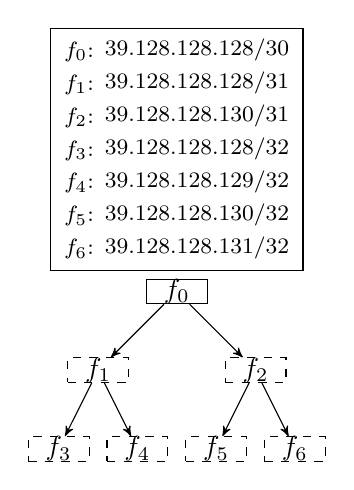
\begin{tikzpicture}[->,>=stealth',level/.style={sibling distance = 2cm/#1,level distance = 1cm}]
            \coordinate (input);
            \node (a) [front, left=3cm of input] {$f_0$}
            child{ node [unexp] {$f_1$} 
                child{ node [unexp] {$f_3$}}
                child{ node [unexp] {$f_4$}}
            }
            child{ node [unexp] {$f_2$} 
                child{ node [unexp] {$f_5$}}
                child{ node [unexp] {$f_6$}}
            };
            \begin{customlegend}[legend cell align=left, legend entries={
                39.128.128.128/30,
                39.128.128.128/31,
                39.128.128.130/31,
                39.128.128.128/32,
                39.128.128.129/32,
                39.128.128.130/32,
                39.128.128.131/32,
            }, legend style={above=0.1cm of a,font=\footnotesize}]
            \addlegendimage{number in legend=$f_0$:}
            \addlegendimage{number in legend=$f_1$:}
            \addlegendimage{number in legend=$f_2$:}
            \addlegendimage{number in legend=$f_3$:}
            \addlegendimage{number in legend=$f_4$:}
            \addlegendimage{number in legend=$f_5$:}
            \addlegendimage{number in legend=$f_6$:}
            \end{customlegend}
            \end{tikzpicture}
        }
    }
    \subfloat[Second epoch usages: $f_1$=7, $f_2$=3] {
        \label{subfig:second_epoch}{
            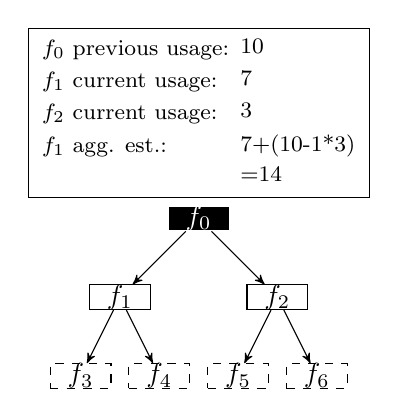
\begin{tikzpicture}[->,>=stealth',level/.style={sibling distance = 2cm/#1,level distance = 1cm}]
            \coordinate (input);
            \node (a) [non_front, left=3cm of input] {$f_0$}
            child{ node [front] {$f_1$} 
                child{ node [unexp] {$f_3$}}
                child{ node [unexp] {$f_4$}}
            }
            child{ node [front] {$f_2$} 
                child{ node [unexp] {$f_5$}}
                child{ node [unexp] {$f_6$}}
            };
            \begin{customlegend}[legend cell align=left, legend entries={
                10,
                7,
                3,
                7+(10-1*3),
                =14,
            }, legend style={above=0.1cm of a,font=\footnotesize}]
            \addlegendimage{number in legend=$f_0$ previous usage:}
            \addlegendimage{number in legend=$f_1$ current usage:}
            \addlegendimage{number in legend=$f_2$ current usage:}
            \addlegendimage{number in legend=$f_1$ agg. est.:}
            \addlegendimage{number in legend=}
            \end{customlegend}
            \end{tikzpicture}
        }
    }
    \hfill
    \subfloat[Last epoch usages: $f_3$=6, $f_4$=1] {
        \label{subfig:last_epoch}{
            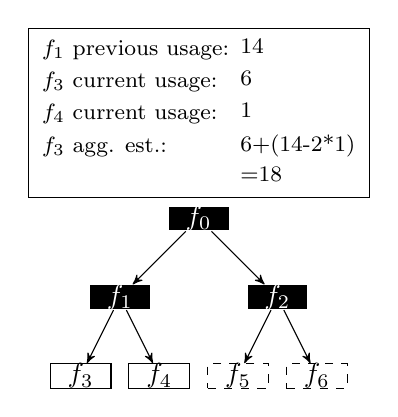
\begin{tikzpicture}[->,>=stealth',level/.style={sibling distance = 2cm/#1,level distance = 1cm}]
            \coordinate (input);
            \node (a) [non_front, left=3cm of input] {$f_0$}
            child{ node [non_front] {$f_1$} 
                child{ node [front] {$f_3$}}
                child{ node [front] {$f_4$}}
            }
            child{ node [non_front] {$f_2$} 
                child{ node [unexp] {$f_5$}}
                child{ node [unexp] {$f_6$}}
            };
            \begin{customlegend}[legend cell align=left, legend entries={
                14,
                6,
                1,
                6+(14-2*1),
                =18,
            }, legend style={above=0.1cm of a,font=\footnotesize}]
            \addlegendimage{number in legend=$f_1$ previous usage:}
            \addlegendimage{number in legend=$f_3$ current usage:}
            \addlegendimage{number in legend=$f_4$ current usage:}
            \addlegendimage{number in legend=$f_3$ agg. est.:}
            \addlegendimage{number in legend=}
            \end{customlegend}
            \end{tikzpicture}
        }
    }
\caption{The algorithm's estimation process at non-first round - closeup look on a subtree}
\label{fig:MultiRoundEstimate}
\end{figure}
\begin{algorithm}
    \SetKwInOut{Input}{Input}
    \SetKwInOut{Output}{Output}
    \Input{A stream of packets $S$. A set of flows $O$. Positive integers $k,R,m$.}
    \Output{top-$k$ flows from $O$ in $S$}
    $F = generate_flowsets(O)$\;
    $number\_rounds=R$\;
    $exact\_flows=\phi$\;
    \ForEach{$round$ in $\{1..number\_rounds\}$}
    {
        $exact\_counters=assign\_exact\_counters(F, \frac{m}{2}, exact\_flows)$\;
        $needed\_epochs=calculate\_needed\_epochs(m, round)$\;
        $packets=get\_round\_packets(round)$\;
        \ForEach{$counter$ in $exact\_counters$}{
            counter\_packets=$\{p\in packets : flow(p)\in counter.flow\}$\;
            counter.value=$\sum\limits_{p \in counter\_packets}size(p)$\;
        }
        \ForEach{$epoch$ in $\{1..needed\_epochs\}$}
        {
            $aggregate\_counters=assign\_aggregate\_counters(F, \frac{m}{2}, epoch,$
            $    round)$\;
            $epoch\_start, epoch\_end=calculate\_epoch\_times(epoch, round)$\;
            $packets=get\_epoch\_packets(epoch\_start, epoch\_end,$
            $    round, exact\_flows)$\;
            \ForEach{$counter$ in $aggregate\_counters$}{
                counter\_packets=$\{p\in packets : flow(p)\in counter.flow\}$\;
                counter.value=$\sum\limits_{p \in counter\_packets}size(p)$\;
            }
            \ForEach{$counter$ in $aggregate\_counters$}{
                $counter.value+=parent\_counter.value-(epoch-1)*sibiling\_counter.value$
            }
            $\{f_i\}^{\frac{m}{2}}_{i=1}=sort(F, aggregate\_counters)$\;
            $F=\bigcup_{i=1}^{i=\frac{m}{4}}refine(f_i)$\;
        }
        $exact\_flows=sort(exact\_flows, exact\_counters,$
         $\{f_i\}^{\frac{m}{2}}_{i=1}, aggregate\_counters)[1:\frac{m}{2}]$\;
    }
    return $exact\_flows[1:k]$\;
    \SetAlgoRefName{``Multi Round''}
    \caption{Solving $ExactTop(S,O,k)$ using $m$ counters.}
    \label{algo:MultiRound}
\end{algorithm}

\section{The \ref{algo:HashNodeExactTop} Algorithm}
The \ref{algo:BasicSplitting} algorithm takes decisions at the end of each epoch. A problematic aspect of this approach that several mid-weighted flows aggregated into a single flowset, might mask a true top-$k$ flow.

\begin{figure}
    \centering
    \subfloat[Measuring $r_0$ and $r_1$ at the first epoch]{\label{subfig:mask_first_epoch}
        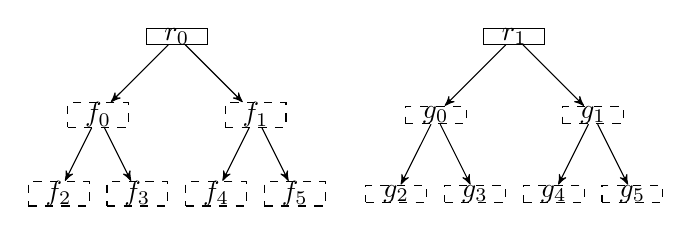
\begin{tikzpicture}[,->,>=stealth',level/.style={sibling distance = 2cm/#1,level distance = 1cm}]
        \coordinate (input);
        \node (a) [front, left=3cm of input] {$r_0$}
        child{ node [unexp] {$f_0$} 
            child{ node [unexp] {$f_2$}}
            child{ node [unexp] {$f_3$}}
        }
        child{ node [unexp] {$f_1$} 
            child{ node [unexp] {$f_4$}}
            child{ node [unexp] {$f_5$}}
        };
        \node (b) [front, right=0.5cm of input] {$r_1$}
        child{ node [unexp] {$g_0$} 
            child{ node [unexp] {$g_2$}}
            child{ node [unexp] {$g_3$}}
        }
        child{ node [unexp] {$g_1$} 
            child{ node [unexp] {$g_4$}}
            child{ node [unexp] {$g_5$}}
        };
        \end{tikzpicture}
    }
    \hfill
    \subfloat[Measurig $g_0$ and $g_1$ at the second epoch]{\label{subfig:mask_second_epoch}
        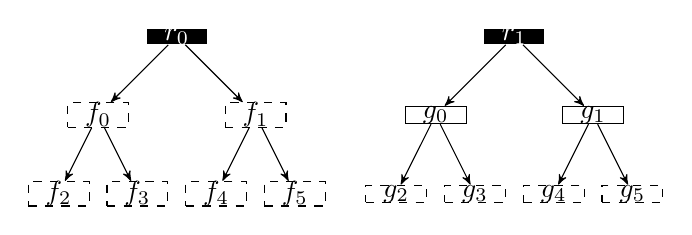
\begin{tikzpicture}[->,>=stealth',level/.style={sibling distance = 2cm/#1,level distance = 1cm}]
        \coordinate (input);
        \node [non_front, left=3cm of input] {$r_0$}
        child{ node [unexp] {$f_0$} 
            child{ node [unexp] {$f_2$}}
            child{ node [unexp] {$f_3$}}
        }
        child{ node [unexp] {$f_1$} 
            child{ node [unexp] {$f_4$}}
            child{ node [unexp] {$f_5$}}
        };
        \node [non_front, right=0.5cm of input] {$r_1$}
        child{ node [front] {$g_0$} 
            child{ node [unexp] {$g_2$}}
            child{ node [unexp] {$g_3$}}
        }
        child{ node [front] {$g_1$} 
            child{ node [unexp] {$g_4$}}
            child{ node [unexp] {$g_5$}}
        };
        \end{tikzpicture}
    }
    \hfill
    \subfloat[Measurig $g_2$ and $g_3$ at the last epoch]{\label{subfig:mask_last_epoch}
        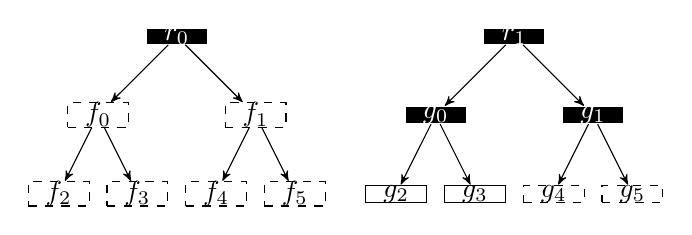
\begin{tikzpicture}[->,>=stealth',level/.style={sibling distance = 2cm/#1,level distance = 1cm}]
        \coordinate (input);
        \node [non_front, left=3cm of input] {$r_0$}
        child{ node [unexp] {$f_0$} 
            child{ node [unexp] {$f_2$}}
            child{ node [unexp] {$f_3$}}
        }
        child{ node [unexp] {$f_1$} 
            child{ node [unexp] {$f_4$}}
            child{ node [unexp] {$f_5$}}
        };
        \node [non_front, right=0.5cm of input] {$r_1$}
        child{ node [non_front] {$g_0$} 
            child{ node [front] {$g_2$}}
            child{ node [front] {$g_3$}}
        }
        child{ node [non_front] {$g_1$} 
            child{ node [unexp] {$g_4$}}
            child{ node [unexp] {$g_5$}}
        };
        \end{tikzpicture}
    }
    \caption{The true heaviest flow (top-$1$) $f_2$ is masked by several mid-weight flows $g_2, g_3, g_4, g_5$.}
    \label{fig:mask}
\end{figure}

Figure~\ref{fig:mask} illustrates such masking situation. In this example, two counters are used to detect the top-$1$ flows (heaviest flow). The arrows between two flowsets indicate a relation of a $refine$ operation. We also assume a constant sizes of $(11, 1, 1, 1, 5, 4, 4, 4)$ for $(f_2, f_3, f_4, f_5, g_2, g_3, g_4, g_5)$ respectively. The correct output for this setup should be $f_2$, but as one can see in this example, the algorithm outputs $g_2$ instead.

Subfigure~\ref{subfig:mask_first_epoch} depicts the first epoch of the monitoring, where the two counters measure the flowsets $r_0$ and $r_1$. At the end of this epoch, the usage values of $r_0$ and $r_1$ are $14$ and $17$ respectively. Thus, at the end of this epoch, the algorithm will assign the counters to measure $g_0$ and $g_1$ in the next epoch.

After this decision had been taken, it is impossible for the algorithm to detect the actual top-$1$ flow. This is true since the algorithm does not have any recovery mechanism. I.e., once it decides not to explore down a branch containing a true top-$k$ flow, it stops assigning counters to that branch and the flow will never be considered again.

Subfigures~\ref{subfig:mask_second_epoch} and ~\ref{subfig:mask_last_epoch} depict the behavior of the algorithm after the crucial wrong decision. They show how it measures $g_0$ and $g_1$ in the second epoch and $g_2$ and $g_3$ in the last epoch. This leads to outputting $g_2$ with usage value of $5$ as the heaviest flow, even though $f_2$ having usage value of $11$.

The probability of such a masking to occur is highest during the very first decisions the algorithm takes. This is true, since the aggregated flowsets gets smaller by half with each new epoch, making it less likely for heavy-weighted flows to be masked by fewer mid-weighted flows.

To overcome the lack of recovery mechanism, which is most evident when such masking occurs, we consider hashing the flows passing through the network node. The hashing process takes place by applying a bijection function $h:2^{\alpha} \rightarrow 2^{\alpha}$, where the flows are defined as strings from $\alpha$.

The idea behind this is to distribute flows of all weights through all of the branches. This prevents the case of heavy aggregated flowsets that do not contain any heavy single flow. Since the output of the algorithm should be the id of the flow as decoded in the packets and the hashed id, the hash must be invertible and thus a bijection.

An important aspect that must be addressed is the ability to implement such a hash function using current switches in line rate.  In order to do so, we limit our implementation to bit-swap hash functions, where several bits in the prefix and suffix of the IP address of the flow are swapped.  It is possible to implement such bit-swap functions using an Experimenter Action in OpenFlow, and the packet handling requires one additional table entry (see~\cite{OF1.5} for more details).

To view the strengths of this approach we revisit the example from Figure~\ref{fig:mask} and consider the behavior of the algorithm while applying the hash function $h = \{f_2\rightarrow g_2, f_3\rightarrow g_4, f_4\rightarrow f_2, f_5\rightarrow f_5, g_2\rightarrow g_5, g_3\rightarrow g_3, g_4\rightarrow f_3, g_5\rightarrow f_4\}$.

\begin{figure}
    \centering
    \subfloat[Measuring $r_0$ and $r_1$ at the first epoch]{\label{subfig:hash_first_epoch}
        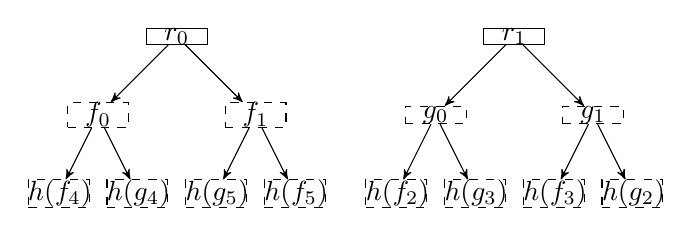
\begin{tikzpicture}[,->,>=stealth',level/.style={sibling distance = 2cm/#1,level distance = 1cm}]
        \coordinate (input);
        \node (a) [front, left=3cm of input] {$r_0$}
        child{ node [unexp] {$f_0$} 
            child{ node [unexp] {$h(f_4)$}}
            child{ node [unexp] {$h(g_4)$}}
        }
        child{ node [unexp] {$f_1$} 
            child{ node [unexp] {$h(g_5)$}}
            child{ node [unexp] {$h(f_5)$}}
        };
        \node (b) [front, right=0.5cm of input] {$r_1$}
        child{ node [unexp] {$g_0$} 
            child{ node [unexp] {$h(f_2)$}}
            child{ node [unexp] {$h(g_3)$}}
        }
        child{ node [unexp] {$g_1$} 
            child{ node [unexp] {$h(f_3)$}}
            child{ node [unexp] {$h(g_2)$}}
        };
        \end{tikzpicture}
    }
    \hfill
    \subfloat[Measurig $g_0$ and $g_1$ at the second epoch]{\label{subfig:hash_second_epoch}
        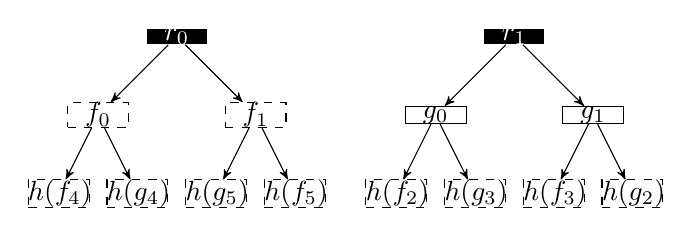
\begin{tikzpicture}[->,>=stealth',level/.style={sibling distance = 2cm/#1,level distance = 1cm}]
        \coordinate (input);
        \node [non_front, left=3cm of input] {$r_0$}
        child{ node [unexp] {$f_0$} 
            child{ node [unexp] {$h(f_4)$}}
            child{ node [unexp] {$h(g_4)$}}
        }
        child{ node [unexp] {$f_1$} 
            child{ node [unexp] {$h(g_5)$}}
            child{ node [unexp] {$h(f_5)$}}
        };
        \node [non_front, right=0.5cm of input] {$r_1$}
        child{ node [front] {$g_0$} 
            child{ node [unexp] {$h(f_2)$}}
            child{ node [unexp] {$h(g_3)$}}
        }
        child{ node [front] {$g_1$} 
            child{ node [unexp] {$h(f_3)$}}
            child{ node [unexp] {$h(g_2)$}}
        };
        \end{tikzpicture}
    }
    \hfill
    \subfloat[Measurig $f_2$ as $h^{-1}(g_2)$ and $g_3$ as $h^{-1}(g_3)$ at the last epoch]{\label{subfig:hash_last_epoch}
        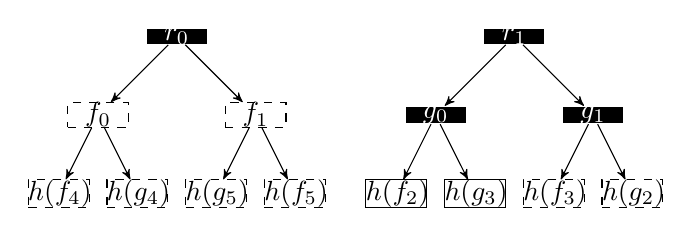
\begin{tikzpicture}[->,>=stealth',level/.style={sibling distance = 2cm/#1,level distance = 1cm}]
        \coordinate (input);
        \node [non_front, left=3cm of input] {$r_0$}
        child{ node [unexp] {$f_0$} 
            child{ node [unexp] {$h(f_4)$}}
            child{ node [unexp] {$h(g_4)$}}
        }
        child{ node [unexp] {$f_1$} 
            child{ node [unexp] {$h(g_5)$}}
            child{ node [unexp] {$h(f_5)$}}
        };
        \node [non_front, right=0.5cm of input] {$r_1$}
        child{ node [non_front] {$g_0$} 
            child{ node [front] {$h(f_2)$}}
            child{ node [front] {$h(g_3)$}}
        }
        child{ node [non_front] {$g_1$} 
            child{ node [unexp] {$h(f_3)$}}
            child{ node [unexp] {$h(g_2)$}}
        };
        \end{tikzpicture}
    }
    \caption{The true heaviest flow (top-$1$) $f2$ is masked by several mid-weight flows $g_2, g_3, g_4, g_5$.}
    \label{fig:hash}
\end{figure}

Subfigure~\ref{subfig:hash_first_epoch} depicts the first epoch of the monitoring, where the two counters measure the flowsets $r_0$ and $r_1$. At the end of this epoch, the sizes of $r_0$ and $r_1$ are $10$ and $21$ respectively. Thus, at the end of this epoch, the algorithm will assign the counters to measure $g_0$ and $g_1$ in the next epoch.

In contrary to the previous scenario, now the heaviest flow $f_2$ is measured in the second epoch, as the flow $h^{-1}(g_2)$. In the second epoch, the sizes of $g_0$ and $g_1$ are $15$ and $6$ respectively. Thus, in the last epoch the algorithm monitors $f_2$ as $h^{-1}(g_2)$ and $g_3$ as $h^{-1}(g_3)$. In the last epoch, the algorithm (instead of outputting $g_2$ as the heaviest flows) outputs $f_2=h^{-1}(g_2)$ which is indeed the heaviest flow.

A two-round algorithm that hashes the flow based on a given hash function is described in Algorithm \ref{algo:HashNodeExactTop}. The algorithm differs from the \ref{algo:MultiRound} Algorithm by the fact that in the second around it uses a given hash function to distribute the flows and prevent masking.

It is worth to note that the function $get\_round\_hash\_function$ actually determines how the flows are hashed. In the first round, this function assigns both $h$ and $h^{-1}$ the identity function and no hashing occurs at the first round. This means, that the first round detects the heaviest $\frac{m}{2}$ flows and assigns them exact counters.

The exclusion of the heaviest flows and the use of hash functions allow the less heavy flows of the true top-$k$ to stand out. Therefore, after the second round, the algorithm holds candidate heaviest $\frac{m}{2}$ flows from the first round and candidate next heaviest $\frac{m}{2}$ flows from the second round.

\begin{algorithm}\small
    \SetKwInOut{Input}{Input}
    \SetKwInOut{Output}{Output}
    \Input{A stream of packets $S$, A set of flows $O$ and positive integers $k, m$.}
    \Output{top-$k$ flows from $O$ in $S$}
    $F = generate\_flowsets(O)$\;
    $number\_rounds=2$\; $exact\_flows=\phi$\;
    \ForEach{$round$ in $\{1..number\_rounds\}$}
    {
        $exact\_counters=assign\_exact\_counters(F, \frac{m}{2}, exact\_flows)$\;
        $needed\_epochs=calculate\_needed\_epochs(m, round)$\;
        $packets=get\_round\_packets(round)$\;
        \ForEach{$counter$ in $exact\_counters$}{
            counter\_packets=$\{p\in packets : flow(p)\in counter.flow\}$\;
            counter.value=$\sum\limits_{p \in counter\_packets}size(p)$\;
        }
        $h, h^{-1}=get\_round\_hash\_function(round)$\;
        \ForEach{$epoch$ in $\{1..needed\_epochs\}$}
        {
            $aggregate\_counters=assign\_aggregate\_counters(F, \frac{m}{2}, epoch, round)$\;
            $epoch\_start, epoch\_end=calculate\_epoch\_times(epoch, round)$\;
            $packets=get\_epoch\_packets(epoch\_start, epoch\_end,$
            $ round, exact\_flows)$\;
            \ForEach{$counter$ in $aggregate\_counters$}{
                counter\_packets=$\{p\in packets : h(flow(p))\in counter.flow\}$\;
                counter.value=$\sum\limits_{p \in counter\_packets}size(p)$\;
            }
            \ForEach{$counter$ in $aggregate\_counters$}{
                $counter.value+=parent\_counter.value-(epoch-1)*sibiling\_counter.value$
            }
            $\{hf_i\}^{\frac{m}{2}}_{i=1}=sort(F, aggregate\_counters)$\;
            $F=\bigcup_{i=1}^{i=\frac{m}{4}}refine(hf_i)$\;
        }
        $\{f_i\}^{\frac{m}{2}}_{i=1}=\{h^{-1}(hf_i)\}^{\frac{m}{2}}_{i=1}$\;
        $exact\_flows=sort(exact\_flows, exact\_counters, \{f_i\}^{\frac{m}{2}}_{i=1},$
        $aggregate\_counters)[1:\frac{m}{2}]$\;
    }
    return $exact\_flows[1:k]$
    \SetAlgoRefName{``Hash then Split''}
    \caption{solving $ExactTop(S,O,k)$ using $m$ counters.}
    \label{algo:HashNodeExactTop}
\end{algorithm}

\section{Results}
\subsection{Setup}
We used \textit{Mininet}~\cite{conf/hotnets/LantzHM10, Mininet} to emulate a software-defined network environment and \textit{Open vSwitch}~\cite{Pfaff2009, OVS} as the OpenFlow enabled switch. \textit{Ryu} SDN framework~\cite{Ryu} was used to build the monitoring application in Python. The setup of the experiments used to evaluate the performance of the algorithms on local node problems was a single switch connected to two hosts via different ports, and the routing entries were set to simply forward traffic from one port to the other.

\textit{Tcpreplay}\footnote{Pcap editing and replaying utilities. available at: http://tcpreplay.appneta.com} was used to replay CAIDA traffic trace~\cite{CAIDA14, CAIDA2016} into the network. Considering the prefixing nature of the algorithm, in order to keep the original characteristics of the real traffic and the privacy of the users, one should be careful to use real traffic traces that went through ``prefix-preserving anonymization'' such as the CAIDA traces.

The traces replayed into the network were slowed down by a factor of $11$ in order to allow the software to cope with the high rate of the recorded traffic and avoid dropping events. Therefore, all timing aspects of the experiments were slowed down by the same factor, and the results are reported in the real timing values rather than the actual ones.

For the evaluation we used two CAIDA traces, from 2014 and 2016\footnote{Data from 2015 was used in the comparison to RAP.}, considering 1-minute interval. The CAIDA'14 trace has the property that the top-$15$ flows are the same $15$ flow throughout every 12-second interval in this minute.
On the other hand, the CAIDA'16 trace has a very significant heavy flow over the whole minute, while the next heaviest flows vary depending on which subinterval is considered. In this sense, the CAIDA'16 trace is an adversarial input due to lack of consistent heavy flows throughout the monitoring intervals.

\subsection{Evaluation of local top-k algorithms}
First, we evaluated the performance of the algorithm \ref{algo:BasicSplitting} on both traces. For that, we conducted a series of experiments to solve $ApproxTop(S,k,\varepsilon)$, with different values of $k$ and $m$ using traffic from both datasets and a constant $\varepsilon=0.05$.

To quantify the performance of the algorithms we define the approximate top-$k$ set ($ATk$), to be the set of flows with frequency higher than $(1-\varepsilon)n_k$, where $n_k$ is the frequency of the $k^{th}$ heaviest flow.
Then the \textit{Detection Rate (DR)} is the percentage of approximate top-$k$ flows the algorithm managed to detect, i.e., $DR=\frac{|f\in output\cap ATk|}{k}$. We note that since all algorithms output exactly $k$ flows, the detection rate is at most $1$.

Figure~\ref{fig:km2014-DR1} depicts the effect of $k$ and $m$ on the detection rate of the algorithm \ref{algo:BasicSplitting} using the CAIDA'14 traces. It is evident that for small values of $k$ the algorithm performs well, achieving a detection rate of at least $0.9$. As expected, for a given number of counters, increasing $k$ decreases the detection rate.
Furthermore, one can see that as the value of $m$ increases the detection rate for a given $k$ also increases, which is expected since the algorithm is using more counters to detect the same heaviest top-$k$ flows.

As expected, when considering experiments with the adversarial traces of CAIDA'16, the performance degrades as seen in Figure~\ref{fig:kmBoth-DR1}. For example, the perfect detection rate for $k=8$ decreases to just above 86\%. Furthermore, the algorithm now needs $128$ counters instead of $32$ to achieve a detection rate about 85\% for $k=12$.

% \begin{figure}
% \subfloat[CAIDA'14 traces \label{fig:km2014-DR1}]{
% \resizebox {0.5\columnwidth} {!} {
% \begin{tikzpicture}
%     \begin{axis}[
%     xlabel={Number of Counters},
%     ylabel={Detection Rate},
%     xtick=data,
%     xticklabels={32, 64, 128, 512},
%     ytick={50,55,60,65,70,75,80,85,90,95,100},
%     legend pos=south east,
%     legend columns=2,
%     ymajorgrids=true,
%     grid style=dashed
%     ]
%     \addplot+[black, mark=o]
%     coordinates {
%         (1,100)(2,100)(3,100)(4,100)
%     };
%     \addlegendentry{$k$=8};
%     \addplot+[black, mark=x]
%     coordinates {
%         (1,90)(2,90)(3,92.5)(4,95)
%     };
%     \addlegendentry{$k$=10};
%     \addplot+[black, mark=|]
%     coordinates {
%         (1,83.3)(2,87.5)(3,85.41)(4,85.41)
%     };
%     \addlegendentry{$k$=12};
%     \addplot+[black, mark=square]
%     coordinates {
%         (1,68.9)(2,75)(3,81.67)(4,83.33)
%     };
%     \addlegendentry{$k$=15};
%     \addplot+[black, mark=triangle]
%     coordinates {
%         (1,61.6)(2,67.5)(3,73.75)(4,77.5)
%     };
%     \addlegendentry{$k$=20};
%     \addplot+[black, mark=diamond]
%     coordinates {
%         (1,58.32)(2,66)(3,75)(4,78)
%     };
%     \addlegendentry{$k$=25};
%     \addplot+[black, mark=pentagon]
%     coordinates {
%         (1,50)(2,67.96)(3,75)(4,75.75)
%     };
%     \addlegendentry{$k$=32};
%     \end{axis}
%     \end{tikzpicture}
% }
% }
% \subfloat[CAIDA'14 + CAIDA'16 traces \label{fig:kmBoth-DR1}]{
% \resizebox {0.5\columnwidth} {!} {
% \begin{tikzpicture}
%     \begin{axis}[
%     xlabel={Number of Counters},
%     ylabel={Detection Rate},
%     xtick=data,
%     xticklabels={32, 64, 128, 512},
%     ytick={40,45,50,55,60,65,70,75,80,85,90},
%     legend pos=south east,
%     legend columns=2,
%     ymajorgrids=true,
%     grid style=dashed
%     ]
%     \addplot+[black, mark=o]
%     coordinates {
%         (1,85)(2,81.25)(3,85.93)(4,84.375)
%     };
%     \addlegendentry{$k$=8};
%     \addplot+[black, mark=x]
%     coordinates {
%         (1,78)(2,78.89)(3,82.5)(4,83.75)
%     };
%     \addlegendentry{$k$=10};
%     \addplot+[black, mark=|]
%     coordinates {
%         (1,73.24)(2,78.125)(3,82.29)(4,83.33)
%     };
%     \addlegendentry{$k$=12};
%     \addplot+[black, mark=square]
%     coordinates {
%         (1,60)(2,68.33)(3,76.67)(4,78.33)
%     };
%     \addlegendentry{$k$=15};
%     \addplot+[black, mark=triangle]
%     coordinates {
%         (1,53)(2,60)(3,70.625)(4,73.75)
%     };
%     \addlegendentry{$k$=20};
%     \addplot+[black, mark=diamond]
%     coordinates {
%         (1,48.36)(2,56)(3,70)(4,73.5)
%     };
%     \addlegendentry{$k$=25};
%     \addplot+[black, mark=pentagon]
%     coordinates {
%         (1,40)(2,52.73)(3,65.23)(4,70.31)
%     };
%     \addlegendentry{$k$=32};
%     \end{axis}
%     \end{tikzpicture}
% }
% }
% \caption{Effects of $k$ and $m$ on the detection rate of Algorithm \ref{algo:BasicSplitting}}
% \end{figure}

\begin{figure}
    \centering
    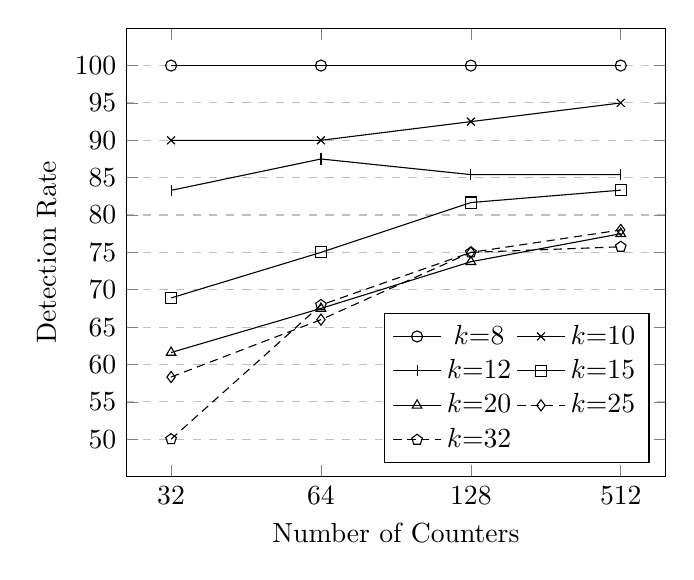
\begin{tikzpicture}
    \begin{axis}[
    xlabel={Number of Counters},
    ylabel={Detection Rate},
    xtick=data,
    xticklabels={32, 64, 128, 512},
    ytick={50,55,60,65,70,75,80,85,90,95,100},
    legend pos=south east,
    legend columns=2,
    ymajorgrids=true,
    grid style=dashed
    ]
    \addplot+[black, mark=o]
    coordinates {
        (1,100)(2,100)(3,100)(4,100)
    };
    \addlegendentry{$k$=8};
    \addplot+[black, mark=x]
    coordinates {
        (1,90)(2,90)(3,92.5)(4,95)
    };
    \addlegendentry{$k$=10};
    \addplot+[black, mark=|]
    coordinates {
        (1,83.3)(2,87.5)(3,85.41)(4,85.41)
    };
    \addlegendentry{$k$=12};
    \addplot+[black, mark=square]
    coordinates {
        (1,68.9)(2,75)(3,81.67)(4,83.33)
    };
    \addlegendentry{$k$=15};
    \addplot+[black, mark=triangle]
    coordinates {
        (1,61.6)(2,67.5)(3,73.75)(4,77.5)
    };
    \addlegendentry{$k$=20};
    \addplot+[black, mark=diamond]
    coordinates {
        (1,58.32)(2,66)(3,75)(4,78)
    };
    \addlegendentry{$k$=25};
    \addplot+[black, mark=pentagon]
    coordinates {
        (1,50)(2,67.96)(3,75)(4,75.75)
    };
    \addlegendentry{$k$=32};
    \end{axis}
    \end{tikzpicture}
    \caption{Effects of $k$ and $m$ on the detection rate of Algorithm \ref{algo:BasicSplitting} - CAIDA'14 traces.}
    \label{fig:km2014-DR1}
\end{figure}

\begin{figure}
    \centering
    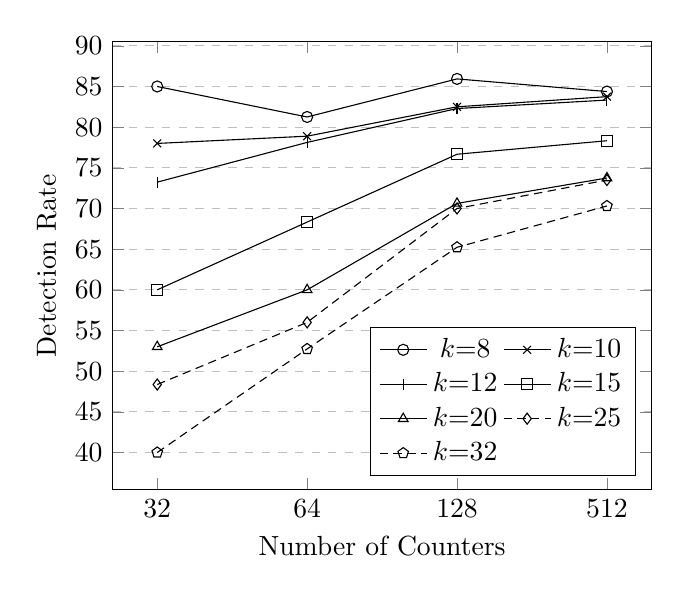
\begin{tikzpicture}
    \begin{axis}[
    xlabel={Number of Counters},
    ylabel={Detection Rate},
    xtick=data,
    xticklabels={32, 64, 128, 512},
    ytick={40,45,50,55,60,65,70,75,80,85,90},
    legend pos=south east,
    legend columns=2,
    ymajorgrids=true,
    grid style=dashed
    ]
    \addplot+[black, mark=o]
    coordinates {
        (1,85)(2,81.25)(3,85.93)(4,84.375)
    };
    \addlegendentry{$k$=8};
    \addplot+[black, mark=x]
    coordinates {
        (1,78)(2,78.89)(3,82.5)(4,83.75)
    };
    \addlegendentry{$k$=10};
    \addplot+[black, mark=|]
    coordinates {
        (1,73.24)(2,78.125)(3,82.29)(4,83.33)
    };
    \addlegendentry{$k$=12};
    \addplot+[black, mark=square]
    coordinates {
        (1,60)(2,68.33)(3,76.67)(4,78.33)
    };
    \addlegendentry{$k$=15};
    \addplot+[black, mark=triangle]
    coordinates {
        (1,53)(2,60)(3,70.625)(4,73.75)
    };
    \addlegendentry{$k$=20};
    \addplot+[black, mark=diamond]
    coordinates {
        (1,48.36)(2,56)(3,70)(4,73.5)
    };
    \addlegendentry{$k$=25};
    \addplot+[black, mark=pentagon]
    coordinates {
        (1,40)(2,52.73)(3,65.23)(4,70.31)
    };
    \addlegendentry{$k$=32};
    \end{axis}
    \end{tikzpicture}
    \caption{Effects of $k$ and $m$ on the detection rate of Algorithm \ref{algo:BasicSplitting} - CAIDA'14 and CAIDA'16 traces}
    \label{fig:kmBoth-DR1}
\end{figure}

Next, we evaluated the effects of several short monitoring rounds instead of a single longer monitoring round, and the effects of hashing the flows. For that, we conducted the same series of experiments each with the appropriate algorithm compared the achieved detection rates. Note that since the Open vSwitch~\cite{OVS} we used in the evaluation does not support (yet) Experimenter Actions we perform the hash directly on the traces.

Figure~\ref{fig:Improvment} depicts the gains in the detection rate for these two approaches compared to the original approach. The horizontal axis marks a set of experiments where the value is the detection rate of the \ref{algo:BasicSplitting} algorithm, while the vertical axis marks the gains the other approaches yielded for this set of experiments.
These results show that both approaches provide gains over the \ref{algo:BasicSplitting} algorithm in different cases. Thus, the combined approach of several rounds and hashing the flows starting from the second round was presented at algorithm \ref{algo:HashNodeExactTop}.

\begin{figure}
\centering
    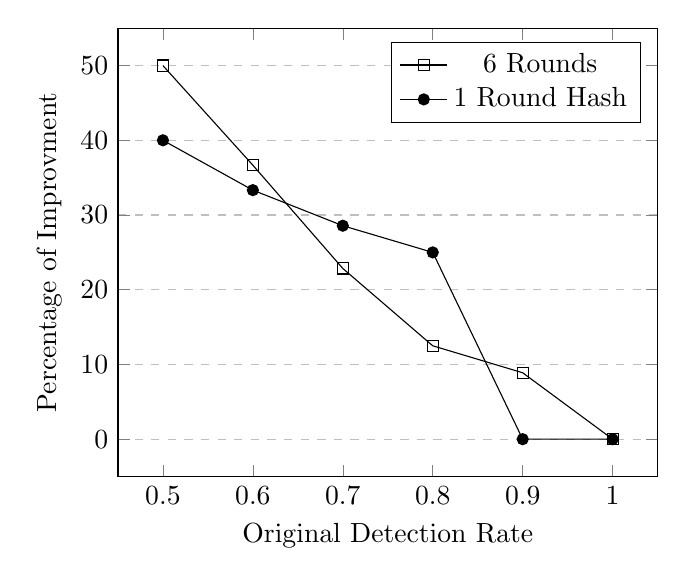
\begin{tikzpicture}
    \begin{axis}[
    xlabel={Original Detection Rate},
    ylabel={Percentage of Improvment},
    xtick={0.5,0.6,0.7,0.8,0.9,1},
    ytick={0,10,20,30,40,50,60},
    legend pos=north east,
    ymajorgrids=true,
    grid style=dashed,
    ]
    \addplot[mark=square]
    coordinates {
        (0.5,50)(0.6,36.67)(0.7,22.85)(0.8,12.5)(0.9,8.89)(1,0)
    };
    \addplot[mark=*]
    coordinates {
        (0.5,40)(0.6,33.33)(0.7,28.57)(0.8,25)(0.9,0)(1,0)
    };
    \legend{6 Rounds, 1 Round Hash}
    \end{axis}
    \end{tikzpicture}
    \caption{Gains in the Detection Rate of the MultiRound and hashing approach against the BasicSplitting $k=10,m=32$.}
    \label{fig:Improvment}
\end{figure}

Figures~\ref{fig:km2014-DR3} and \ref{fig:kmBoth-DR3} show the effect of $k$ and $m$ on the detection rate of the algorithm \ref{algo:HashNodeExactTop} for CAIDA'14 and both traces, respectively. One can see that the same trends we noted regarding the performance of algorithm \ref{algo:BasicSplitting} also hold for this case. Furthermore, these figures also show the superiority of the algorithm \ref{algo:HashNodeExactTop} over the algorithm \ref{algo:BasicSplitting} in all settings.

\begin{figure}
    \centering
    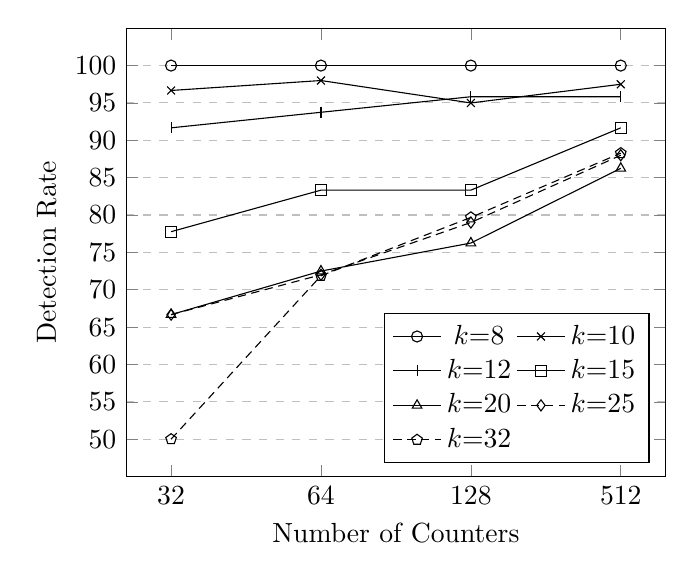
\begin{tikzpicture}
    \begin{axis}[
    xlabel={Number of Counters},
    ylabel={Detection Rate},
    xtick=data,
    xticklabels={32, 64, 128, 512},
    ytick={50,55,60,65,70,75,80,85,90,95,100},
    legend pos=south east,
    legend columns=2,
    ymajorgrids=true,
    grid style=dashed
    ]
    \addplot+[black, mark=o]
    coordinates {
        (1,100)(2,100)(3,100)(4,100)
    };
    \addlegendentry{$k$=8};
    \addplot+[black, mark=x]
    coordinates {
        (1,96.67)(2,98)(3,95)(4,97.5)
    };
    \addlegendentry{$k$=10};
    \addplot+[black, mark=|]
    coordinates {
        (1,91.67)(2,93.75)(3,95.83)(4,95.83)
    };
    \addlegendentry{$k$=12};
    \addplot+[black, mark=square]
    coordinates {
        (1,77.77)(2,83.33)(3,83.33)(4,91.67)
    };
    \addlegendentry{$k$=15};
    \addplot+[black, mark=triangle]
    coordinates {
        (1,66.67)(2,72.5)(3,76.25)(4,86.25)
    };
    \addlegendentry{$k$=20};
    \addplot+[black, mark=diamond]
    coordinates {
        (1,66.67)(2,72)(3,79)(4,88)
    };
    \addlegendentry{$k$=25};
    \addplot+[black, mark=pentagon]
    coordinates {
        (1,50)(2,71.87)(3,79.68)(4,88.28)
    };
    \addlegendentry{$k$=32};
    \end{axis}
    \end{tikzpicture}
    \caption{Effects of $k$ and $m$ on the detection rate of Algorithm \ref{algo:HashNodeExactTop} - CAIDA'14 traces.}
    \label{fig:km2014-DR3}

\end{figure}

\begin{figure}
    \centering
    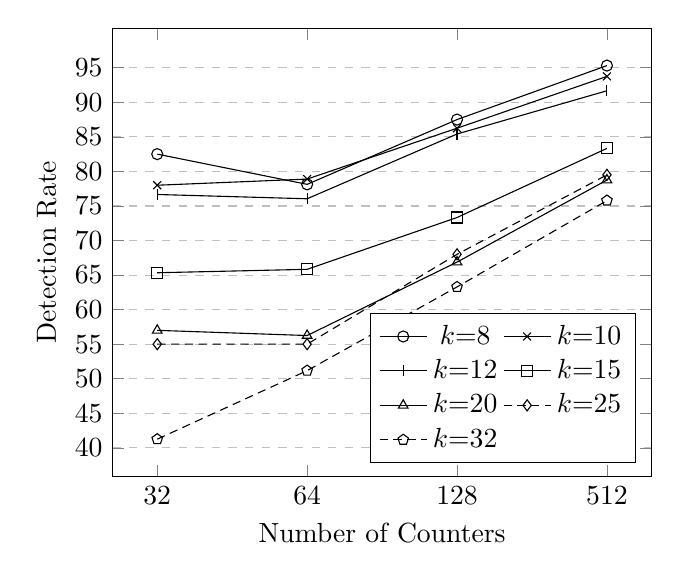
\begin{tikzpicture}
    \begin{axis}[
    xlabel={Number of Counters},
    ylabel={Detection Rate},
    xtick=data,
    xticklabels={32, 64, 128, 512},
    ytick={40,45,50,55,60,65,70,75,80,85,90,95},
    legend pos=south east,
    legend columns=2,
    ymajorgrids=true,
    grid style=dashed
    ]
    \addplot+[black, mark=o]
    coordinates {
        (1,82.5)(2,78.125)(3,87.5)(4,95.3125)
    };
    \addlegendentry{$k$=8};
    \addplot+[black, mark=x]
    coordinates {
        (1,78)(2,78.89)(3,86.25)(4,93.75)
    };
    \addlegendentry{$k$=10};
    \addplot+[black, mark=|]
    coordinates {
        (1,76.66)(2,76.04)(3,85.41)(4,91.67)
    };
    \addlegendentry{$k$=12};
    \addplot+[black, mark=square]
    coordinates {
        (1,65.334)(2,65.83)(3,73.33)(4,83.33)
    };
    \addlegendentry{$k$=15};
    \addplot+[black, mark=triangle]
    coordinates {
        (1,57)(2,56.25)(3,66.875)(4,78.75)
    };
    \addlegendentry{$k$=20};
    \addplot+[black, mark=diamond]
    coordinates {
        (1,55)(2,55)(3,68)(4,79.5)
    };
    \addlegendentry{$k$=25};
    \addplot+[black, mark=pentagon]
    coordinates {
        (1,41.25)(2,51.17)(3,63.28)(4,75.78)
    };
    \addlegendentry{$k$=32};
    \end{axis}
    \end{tikzpicture}
    \caption{Effects of $k$ and $m$ on the detection rate of Algorithm \ref{algo:HashNodeExactTop} - CAIDA'14 and CAIDA'16 traces}
    \label{fig:kmBoth-DR3}
\end{figure}

\subsection{Comparison to state of art streaming algorithms}
The RAP family of algorithms introduced recently in \cite{Ben-Basat2017} are the best performing top-$k$ streaming algorithms. As mentioned in the Introduction, these algorithms require per packet operations and complex data structures, and even when adapted to perform (i.e., dW-RAP) in line-rate they exhibit low precision rate (of about 50\%). Moreover, these algorithms are designed to address the packet rate version of the problem. 
 
Still, it is important to compare the expected performance of our algorithm that use only available counters and works well also on the traffic rate version. In \cite{Ben-Basat2017} the evaluation was done on several traces, where CAIDA’15~\cite{CAIDA15} being the dominant real-world trace. The reported experiments included a convergence period and the results depend on the number of packets in the experiment. Since our algorithms are not confined by the number of packets but by time considerations (since this is the way monitoring is done in the industry) we had to slightly modify our algorithms to allow a comparison. We changed the algorithms’ epochs and rounds to be based on the number of packets passed rather than on time units. Figure~\ref{fig:RAP} compares the detection rate of RAP and the \ref{algo:HashNodeExactTop} algorithms in this modified setting for the same CAIDA’15~\cite{CAIDA15} traces when the goal is the packet based top-$k$ flows. Note that dW-RAP uses a metadata field (flow ID) and we use very basic counters – thus in order to compare we assume that pointers to metadata have the same size as counters. One can see that for this objective and the same amount of memory there is no big difference, \ref{algo:HashNodeExactTop} performs a bit better for a small number of counters and a bit worse for large numbers. 

However, when we implemented RAP for the more relevant traffic metric the picture is a bit different.  As already mentioned in the paper, it is not straightforward to support packet size and total bit count of flows while keeping the deterministic and probabilistic bounds of RAP, so we had to modify the criterion for flow eviction to be a probabilistic function of the amount of bytes in the traffic instead of the number of packets. As depicted in Figure~\ref{fig:BWRAP}, \ref{algo:HashNodeExactTop} performs significantly better than the weighted version of RAP (denoted BW-RAP) in all settings when the number of counters is less than 512. If more than 512 counters are available then both algorithms achieve almost the same high detection rate. 

\begin{figure}
    \centering
    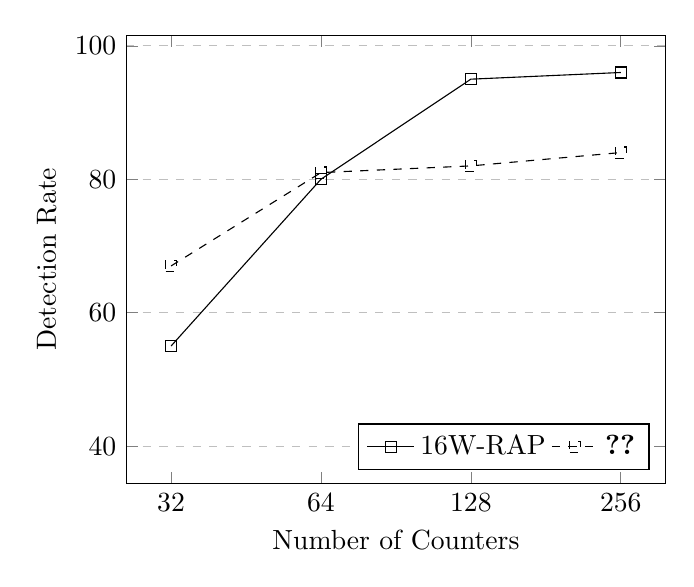
\begin{tikzpicture}
    \begin{axis}[
    xlabel={Number of Counters},
    ylabel={Detection Rate},
    xtick=data,
    xticklabels={32, 64, 128, 256},
    ytick={40,60,80,100},
    legend pos=south east,
    legend columns=2,
    ymajorgrids=true,
    grid style=dashed
    ]
    \addplot+[white, mark=none, draw=none, forget plot]
    coordinates {
        (1,40)(2,40)(3,40)(4,40)
    };
    \addplot+[black, mark=square]
    coordinates {
        (1,55)(2,80)(3,95)(4,96)
    };
    \addlegendentry{16W-RAP};
    \addplot+[black, mark=square, dashed]
    coordinates {
        (1,67)(2,81)(3,82)(4,84)
    };
    \addlegendentry{\ref{algo:HashNodeExactTop}};
    \end{axis}
    \end{tikzpicture}
    \caption{Comparison of Detection Rate for finding top-$32$ flows vs. number of counters - CAIDA'15 traces}
    \label{fig:RAP}

\end{figure}

\begin{figure}
    \centering
    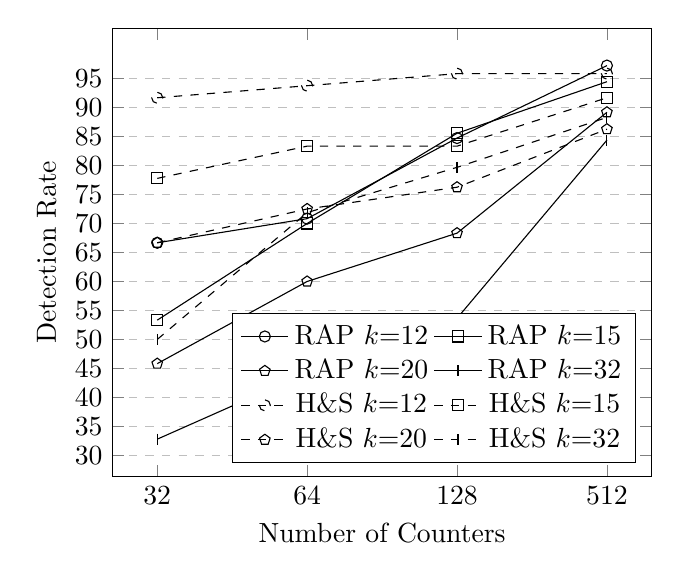
\begin{tikzpicture}
    \begin{axis}[
    xlabel={Number of Counters},
    ylabel={Detection Rate},
    xtick=data,
    xticklabels={32, 64, 128, 512},
    ytick={30,35,40,45,50,55,60,65,70,75,80,85,90,95},
    legend pos=south east,
    legend columns=2,
    ymajorgrids=true,
    grid style=dashed
    ]
    \addplot+[black, mark=o]
    coordinates {
        (1,66.67)(2,70.83)(3,84.72)(4,97.22)
    };
    \addlegendentry{RAP $k$=12};
    \addplot+[black, mark=square]
    coordinates {
        (1,53.33)(2,70)(3,85.55)(4,94.44)
    };
    \addlegendentry{RAP $k$=15};
    \addplot+[black, mark=pentagon]
    coordinates {
        (1,45.83)(2,60)(3,68.33)(4,89.17)
    };
    \addlegendentry{RAP $k$=20};
    \addplot+[black, mark=|]
    coordinates {
        (1,32.81)(2,44.27)(3,53.65)(4,84.37)
    };
    \addlegendentry{RAP $k$=32};
    \addplot+[black, mark=o, dashed]
    coordinates {
        (1,91.67)(2,93.75)(3,95.83)(4,95.83)
    };
    \addlegendentry{H\&S $k$=12};
    \addplot+[black, mark=square, dashed]
    coordinates {
        (1,77.77)(2,83.33)(3,83.33)(4,91.67)
    };
    \addlegendentry{H\&S $k$=15};
    \addplot+[black, mark=pentagon, dashed]
    coordinates {
        (1,66.67)(2,72.5)(3,76.25)(4,86.25)
    };
    \addlegendentry{H\&S $k$=20};
    \addplot+[black, mark=|, dashed]
    coordinates {
        (1,50)(2,71.87)(3,79.68)(4,88.28)
    };
    \addlegendentry{H\&S $k$=32};
    \end{axis}
    \end{tikzpicture}
    \caption{Comparison of \ref{algo:HashNodeExactTop} and BW-RAP algorithms - CAIDA'14 and CAIDA'16 traces}
    \label{fig:BWRAP}

\end{figure}

\section{Related Work}
Formally, the top-$k$ problem aims at finding the top-$k$ elements that have the highest frequency from a stream of elements. The space requirements for an exact solution to this problem are impractical~\cite{Charikar2004} and thus many relaxations of the original problem were proposed.

The $FindCandidateTop(S, k, l)$ problem was proposed in~\cite{Charikar2004} defining the $l$ elements among which the top-$k$ elements are concealed, with no guarantees on the rank of the remaining $l-k$ elements. While the more practical approximation $FindApproxTop(S, k, \varepsilon)$, also proposed in~\cite{Charikar2004} requires a list of $k$ elements, where every element in the list has a frequency within $(1-\varepsilon)$ of the $k^{th}$ element frequency.

To evaluate the performance of algorithms solving these approximations, two parameters were proposed~\cite{Cormode2005} (in addition to the space requirement): \textit{recall,} the number of correct elements found as a percentage of the number of actual correct elements; and the \textit{precision}, the number of correct elements found as a percentage of the entire output.

% The \textit{Frequent} algorithm proposed in~\cite{Demaine2002} outputs a list of $k$ elements with no guarantee on the elements frequency. It keeps $k$ counters to monitor $k$ elements, if a monitored element is observed, its counter is incremented, else all counters are decremented.
% If a counter reaches $0$, it is assigned the next observed element. When the algorithm terminates, the monitored elements are the candidate frequent elements. A significant contribution of this work was the proposed lightweight data structure (a doubly linked list) that can decrement all counters in $O(1)$ operations.
% The main drawback of this approach is the usage of dynamically allocated memory and pointers for the lightweight data structure, which makes difficult to implement on network nodes.

Metwally et al. proposed the \textit{Space-Saving} algorithm in~\cite{Metwally2005}. It builds on the ideas of \textit{Frequent}~\cite{Demaine2002} while improving the time complexity of looking up a value of a counter from $O(m)$ to $O(1)$. The main difference from \textit{Frequent} is that when a non-monitored item arrives, the algorithms assign it the minimal counter while preserving its value. They proved that regardless of the data distribution, \textit{Space-Saving} needs $min(|A|,\frac{N}{\varepsilon F_k})$ counters to correctly solve $FindApproxTop(S, k, \varepsilon)$. Where $A$ is the elements universe, $N$ is the size of the stream and $F_k$ is the frequency of the $k^{th}$ element. When considering high volume network traffic, the value of $|A|$ is at least $2^{32}$ while $\frac{N}{F_k}$ can be very high depending on the traffic's characteristics, thus the number of counters can be unrealistically high.

Ben-Basat et al.~\cite{Ben-Basat2017} introduced the \textit{Randomized Admission Policy (RAP)} algorithm which randomly decides if to reassign a counter to measure non-monitored items. The probability of reassigning a counter is in inverse relation to the counter's value. The motivation behind this reassignment policy is that infrequent non-monitored items will need to arrive several consecutive times to replace a monitored item. The authors acknowledge the difficulty of implementing RAP in hardware and presented a hardware-friendly variant, \textit{d-Way Randomized Admission Policy (dW-RAP)}, which performs poorer than RAP. This variant assumes the existence of $d$-way associative cache in the node's hardware, where its entries can be partitioned to store metadata (ID) and value.

Several other recent works have also focused on efficient resource-constrained flow monitoring, realizing that measurement is crucial for network management and control and even more so in the SDN domain~\cite{Moraney2016, Moshref2013, Moshref2014}. Moraney and Raz introduced in~\cite{Moraney2016} an efficient scheme to detect flow anomalies, based on a variation of the MRT algorithm presented in~\cite{Moshref2014}. The scheme used a constant number of counters, in periodic assessment and reassignment fashion, to detect anomalous flows regardless of the number of active flows.

In~\cite{Moraney2016} an efficient anomaly detection mechanism was introduced. The mechanism is based on detecting ``over-usage" in regards to flows, i.e., flows that surpass a given threshold. While such a mechanism is efficient in detecting flows that have a certain individual property, it is not usable in detecting flows that uphold a global property such as top-$k$ flow. Furthermore, the authors assumed a given application-specific threshold that defines when the local property holds. However, setting such thresholds is a non-trivial hard task since they need to capture the various aspects of the anomaly and the traffic.

The authors of~\cite{Moshref2013} concentrated on the tradeoff between the amount of available resources and the accuracy of the measurement. Note, that like many of the works in this area, they do not present an analytical framework to study this tradeoff and rather concentrated on important system related issues.
The same authors proposed more recently in~\cite{Moshref2014} a network wise dynamic monitoring system where the SDN controller dynamically configures monitoring rules in the different network elements. Such a centralized management entity can thus make use of global information in order to utilize the distributed monitoring resources (typically TCAM rules) in an efficient way, that is, getting as much precision as possible for the given monitoring resources.

\section{Conclusions}
In this paper, we develop a family of practical, efficient memory-constrained algorithms for detecting the top-$k$ flows in terms of total traffic rate. These algorithms use built-in counters available in any switching node and are deployable “out of the box” on any OpenFlow enabled node. We evaluated the expected performance of these algorithms using real-life packet traces, and the evaluation shows that our new algorithms achieve high detection rates while maintaining full precision regardless of the packet rate. We also show that for the top-$k$ packet rate problem these algorithms perform as well as the best streaming algorithms that use complex data structures and much more elaborated computations. Moreover, for the more relevant weighted top-$k$ problem our algorithms outperform state-of-the-art streaming algorithm when evaluated over recent real traffic. 

One future direction is to use this infrastructure as a building-block for detecting network-wise top-$k$ flows. We believe that combining the local performance described in this paper with a smart global policy about the number of counters to be used in each node, will lead to a deployable memory-efficient monitoring system for efficient detection of network-wise top-$k$ flows.







\chapter{On the Practical Detection of Hierarchical Heavy Hitters}
\section{Absract}
Finding the network's heaviest flows is an important and challenging network monitoring task and a critical building block for many other applications.
In the hierarchical heavy hitters (HHH) problem, one needs to identify the most frequent network IP-prefixes hierarchically.
This is a challenging task since the number of relevant IP-prefixes of flows in a busy router is much higher than the number of counters.
To address this point, many streaming algorithms were recently developed, but they use complex data-structures and usually have non-constant per-packet update-time, preventing them from being deployed in line-speed.
A randomized constant-time algorithm was proposed recently; however, it is only applicable to extremely large streams.

In this paper, we propose a constant-time algorithm for detecting the HHH that does not have any convergence requirements and achieves comparable results to state of the art.
Furthermore, our algorithm uses only efficient built-in counters available in current network devices, making it deployable on commercially off-the-shelf network gear.
We provide an analytical study of the problem and show, using emulation over real traffic, that our algorithm performs at least as well as the best-known streaming algorithms without performing expensive per-packet operations or requiring convergence periods.
\section{Introduction}
\ignore{
The increasing popularity of cloud based systems and the shift towards Infrastructure as a Service (IaaS)  as the preferred  solution for many organizations~\cite{Goyal2013}, requires new approaches and novel solutions in the area of system  management. Efficient management of such infrastructure heavily rely  on  efficient monitoring of the system resources and the workload. Despite many previous works considering efficiency aspects of many network management systems~\cite{devoflow, microte, anomaly}, very few tackled the practicality of deploying efficient monitoring tasks.

A practical efficient algorithm for any network monitoring task requires: (1) to be deployable on off the shelf network nodes, (2) to cope with current line rates, and finally (3) to use a limited amount of network resources which is much smaller than the ever increasing number of active flows.
}

The detection of hierarchical heavy hitters flows is an important monitoring task that was in the spotlight of recent research~\cite{ben2016heavy, basat2017optimal, ben2017constant, sivaraman2017heavy, HHHOnline, tong2015high}. A Heavy Hitter is a flow that is responsible for a considerable portion of the overall traffic (i.e., flows with traffic that exceeds a certain threshold) and a Hierarchical Heavy Hitter is an aggregation of non-HH flows that share common property and is responsible, as a whole, for traffic above the threshold.

The algorithms presented in this chapter takes advantage of the ability to reconfigure counters over time in network nodes. These reconfigurations, take place at statically provisioned periods of times, called rounds, depending on the given monitoring interval.
During the rounds, the allocated counters simply measure the traffic of the assigned aggregated prefix. Thus, the per-packet operation can be handled in line rate with no additional support of special data structures or specialized hardware. Furthermore, we exploit the fact that these counters can measure both the number of packets and the total byte count with no additional cost in order to also solve the weighted version of the problem.

We present four algorithms, following the steps of~\cite{conf/sigcomm/YuanCM07,Moraney2016} and the work introduced in the previous chapter. In the first algorithm, we assign to each counter an aggregated set of flows starting from some level of the hierarchy. At the end of each round, the algorithm seeks to zoom in on interesting flows down the hierarchy,  thus evaluates the counters' values and reassigns the counters to the top half of the counters for the new round. The second algorithm aims at improving the performance by increasing the length of each round and decreasing the number of rounds. The motivation is that longer rounds lead to more stable HH and the zooming in process is more accurate.

Our third algorithm remedies a major limitation of the first two algorithms, the lack of a ``reconsidering" mechanism. I.e., the ability of the algorithm's to back off from the zooming process if the found flows turned out to be uninteresting and allocate the counter to previously discarded flow. This is achieved by keeping the frontier of the hierarchy disjointly monitored by counters over different levels.
The fourth algorithm waives the request of disjointly monitoring the frontier by monitored the highest shared ancestor that does not surpass the threshold. The motivation is to reduce the number of counters needed to cover the frontier and to enable deploying the algorithm when fewer counters are available.

The result is a family of practical efficient monitoring algorithms to the HHH problem which are deployable on off the shelf network nodes (see~\cite{Moraney2016} for the practicality of the approach) and can operate in line speed due to its constant time per-packet update operation. Furthermore, the algorithms use a configurable constant number of counters and guarantee not to use more than the allocated counters.

We evaluate the expected performance of our algorithms on real network traffic through an extensive simulation study using CAIDA’s traces~\cite{CAIDA2016, CAIDA2018}.
The results indicate that our algorithms can detect around 90\% of the true HHH while reporting only 3\% non-HHH flows. These results can be achieved in line rate, while not requiring any convergence interval. Also, these results are comparable to the state of the art algorithms: (1)``MST"~\cite{SpaceSaving} - an accurate Space Saving~\cite{Metwally2005} based algorithm that can not be deployed in line rate due to non-constant per-packet update operation, and (2)``RHHH"~\cite{ben2017constant} a probabilistic constant update time improvement of ``MST" that requires a large convergence interval of 100M packets.

The rest of this chapter is organized as follows; First, we survey related work, then we provide the notations and define formally the problem. Afterwards, we present our four algorithms: the~\ref{algo:simple_split}, the~\ref{algo:multiple_split}, the~\ref{algo:htf} and the~\ref{algo:sa} algorithms. Finally, we evaluate the performance of the algorithms and compare them to the state of the art.

\section{Related Work}
Various papers had addressed the efficient detection of Hierarchical Heavy Hitters in the fields of streaming data and network monitoring. These papers dealt with many aspects of the problem, including but not limited to (1) The number of dimensions of the hierarchy, (2) Relaxation of the problem by approximation, (3) Space requirements of the algorithms, (4) per item (packet) update time, (5) Lower bound on required Space, and (6) Convergence requirements of the algorithms.

The single dimension variant of the problem was introduced
and approximated by a streaming algorithm in~\cite{HHHInStreams}.
Later, ~\cite{separator} introduced an algorithm that requires $O(H^2/\epsilon)$ space, where $H$ is the depth of the hierarchy and $\epsilon$ is the allowed relative estimation error for each single flow frequency.

Many algorithms to solve the multiple dimensions variant of the problem were proposed, each with its own properties ~\cite{HHHOnline, SpaceSaving, HHHInStreams-MultiDimension, weightedCircuits, MultiDimensionHHH, lowerboundsonMultiDimension}. The common property of these algorithms is that the depth of the multi-dimensional hierarchy is the product of each dimension.

In ~\cite{HHHOnline}, trie based algorithms were proposed that requires $O(H)$ update time, space of $O(H^2/\epsilon)$ and  maintains a special data structure to hold the trie and its dynamic expansion. More recently, another trie-based solution was introduced in ~\cite{HHHInStreams-MultiDimension}, the Full Ancestry and Partial Ancestry, that use $O(Hlog(N\epsilon)/\epsilon)$ space and requires $O(Hlog(N\epsilon))$ time per update, where $N$ is the stream length. Alternatively, ~\cite{weightedCircuits} improve the required space and update time to $O(H^{3/2}/\epsilon)$ (regardless of $N$) for the two dimensional problem.

A more efficient sketch-based algorithm with strong error and space guarantees were proposed in ~\cite{SpaceSaving}. In their approach, they utilized a copy of Space Saving Sketch~\cite{metwally2005efficient} per level, and detected the hierarchical heavy hitters by detected heavy hitters throughout all levels of the hierarchy. The algorithm requires $O(H/\epsilon)$ space and $O(H)$ update time~\footnote{In the weighed version the update time is $O(Hlog(1/\epsilon))$}.

Recently, a probabilistic version of the hierarchical heavy hitters problem was described in~\cite{ben2017constant}. Exploiting this definition, the algorithm improved the update time to $O(1)$ on the expense of requiring a convergence interval. That is, a minimal number of items has to be processed before the probabilistic guarantees of the algorithm hold. The authors argue that in practice the algorithm's output is of the same quality as the previous deterministic approaches, while the convergence interval is not a real limitation since modern networks route a continuously increasing number of packets.

DREAM~\cite{Moshref2014} is a framework for dynamically scheduling network traffic monitoring jobs (as black boxes), by allocating the amount of resources needed to maintain the predetermined accuracy of each job. When a monitoring job with a given accuracy requires more resources than  available in the switch, the framework either rejects the job or tries to perform an expensive multi-switch resource allocation to achieve the desired accuracy rates.
Such framework effectively balances two of the most critical characteristics of monitoring jobs, resources' availability and monitoring accuracy, and it is a very important and useful tool  to schedule monitoring jobs in a compatible manner.

Our paper describes a different approach to detect hierarchical heavy hitters,
while still being usable as a black box monitoring job in scheduling frameworks such as DREAM. The main trait of the approach is the practicality of deploying our algorithms on off-the-shelf network nodes while using a given number of counters (space) to detect the hierarchical heavy hitters. Furthermore, the per-packet update time of the proposed algorithms is $O(1)$ without requiring any special data-structure or any convergence interval.
\section{Notations and Problem Definition}

A  \textit{flow} is a set of packets that share a common property (usually IP header fields).  For example, all packets that have the same IP\_SRC address belong to the same flow. One can form a hierarchy of flows by considering  the prefixes  of the field that specify a flow. In our example, the prefixes of the IP\_SRC addresses forms the hierarchy.  More formally,  the   universe of flows, $\mathcal U$, forms a hierarchy where the \textit{dimensions} of the hierarchy is the number of fields that defines the flow and the \textit{hierarchy levels} are the various prefixes of the fields values.  Using this definition the flows in our example are of a single dimension (we only consider one field in the header) and a flow at level $l$ consists of all packets that share the same prefix of length $l$ from the IP\_SRC field.

In order to formally define the hierarchy, we define the \textit{Generalization Relation} between two hierarchy elements $p,q$, denoted by $p \prec q$, and say that $p$ generalizes $q$, if $p$ is a proper prefix of $q$ with respect to a specific dimension (i.e., a field in the packet header).  The \textit{hierarchy depth}, $H$, is the length of the maximal path of prefixes that confirms with this generalization relation. In our example, the depth of the hierarchy is $32$ as there are $32$ bits in an IP address. 

Given a \textit{stream} of packets, $\mathcal S$ (sometimes referred to also as a trace) one can ask what is the frequency of a given flow in that stream. That is, how many packets that belong to this specific flow appear in the stream. In the case of streams of packets we also consider the weighted version of the frequency of a flow, which is the total amount of bytes carried by packets that belong to this flow.  We use $T$ to donate the total frequencies of all elements, $N$ to denote the overall number of packets in the stream, and $B$ to denote the total amount of bytes in the stream. Usually $T=N$, however when we consider the weighted frequencies of flows $T=B$.

Given a threshold $\phi$, an element of the hierarchy (either a prefix or a specific flow) $x$, is a \textit{Heavy Hitter (HH)} if its frequency is at least $\phi$ of the total frequencies of all elements, i.e., $f_x \geq \phi T$. The \textit{Conditioned frequency} of prefix $p$ with respect to a set of prefixes $P$, $cf_p(P)$, is the sum of frequencies of all elements that $p$ generalizes without those of $P$. That is, we subtract from the frequency of $p$ the sum of frequencies of the flows that are generalized by elements of the set $P$.

Given a threshold $\phi$, an element of the hierarchy (either a prefix or a specific flow) is a \textit{Hierarchical Heavy Hitter (HHH)} if its conditioned frequency with respect to the set of HHH  is at least $\phi T$.  Another way to define the set of HHH for a given a stream of packets and a threshold $\phi$, is to build it recursively. The set $HHH_H$ is the set of HH at the lowest level of the hierarchy, i.e., $HHH_H=\{x\in \mathcal U| f_x \geq \phi T\}$. The set $HHH_l$, is the set of all prefixes at level $l$ that their conditional frequency with respect to $HHH_{l+1}$ is at least $\phi T$, i.e., $HHH_l=\{p \text{ at level } l | cf_p(HHH_{l+1}) \geq \phi T\}$. Then, the set of all HHH from all the levels of the hierarchy is $HHH=\bigcup_{l=0}^{H}HHH_l$.
 Table~\ref{tab:def} contains the list of symbols and notations we use throughout this paper.
\begin{table}[ht]
	%\footnotesize
	\centering{
	\resizebox{1.0 \columnwidth}{!}{
	\begin{tabular}{|c|l|}
		\hline
		Symbol & Meaning \tabularnewline
		\hline
		$\mathcal U$ & The universe of flow identifiers \tabularnewline
		\hline
		$\mathcal S$ & The stream of packets \tabularnewline
		\hline
		$T$ & The total frequencies in $\mathcal S$\tabularnewline
		\hline		
		$N$ & The overall number of packets in $\mathcal S$\tabularnewline
		\hline		
		$B$ & The total byte count of packets in $\mathcal S$\tabularnewline
		\hline
		$f_x$ & The frequency of flow $x\in\mathcal U$ \tabularnewline
		\hline
		$cf_p(P)$ & The conditional frequency of $p$ in respect to $P$ \tabularnewline
		\hline
		$\phi$ & Heavy Hitter threshold  \tabularnewline
		\hline	
	    $H$ & The depth of the hierarchy \tabularnewline
		\hline
		$p \prec q$ & $p$ generalize $q$ in the hierarchy \tabularnewline
		\hline
		$C$ & The number of available counters \tabularnewline
		\hline
	\end{tabular}
	}	
}
	\caption{A list of symbols and notations}
	\label{tab:def}
\end{table}
%\normalsize 

\section{The \simpleAlgo Algorithm}

In general, the term \textit{flowset}~\cite{conf/sigcomm/YuanCM07} is used to describe the stream formed from an aggregation of flows.
In the context of this chapter, we are interested only in flowsets that cover a full hierarchy.
Furthermore, it is very practical to assign counters to measure flowsets that cover a full hierarchy, using wild-cards matching techniques widely available in any traditional network gear and over the shelf SDN switches~\cite{OVS, OF1.5}.

\begin{figure}
	\centering
    \subfloat[The hierarchical flowset $f_3 \cup f_4\cup f_5\cup f_6$ can be measured by measuring $f_0$.]{
        \label{subfig:hierarchical_flowset}{
            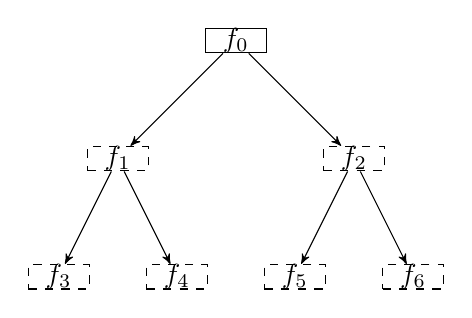
\begin{tikzpicture}[->,>=stealth',level/.style={sibling distance = 3cm/#1,level distance = 1.5cm}]
            \coordinate (input);
            \node (a) [front, left=3cm of input] {$f_0$}
            child{ node [unexp] {$f_1$} 
                child{ node [unexp] {$f_3$}}
                child{ node [unexp] {$f_4$}}
            }
            child{ node [unexp] {$f_2$} 
                child{ node [unexp] {$f_5$}}
                child{ node [unexp] {$f_6$}}
            };
            \end{tikzpicture}
        }}
    \subfloat[The non Hierarchical flowset $f_3 \cup f_4 \cup f_6$, requires at least measuring $f_1$ and $f_6$.] {
        \label{subfig:HHH_second_epoch}{
            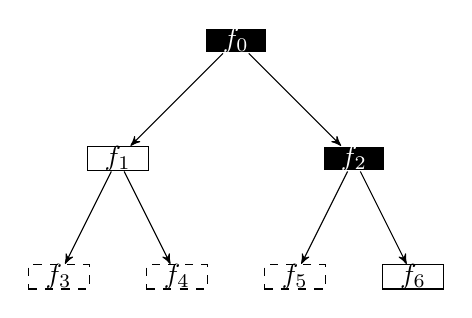
\begin{tikzpicture}[->,>=stealth',level/.style={sibling distance = 3cm/#1,level distance = 1.5cm}]
            \coordinate (input);
            \node (a) [non_front, left=3cm of input] {$f_0$}
            child{ node [front] {$f_1$} 
                child{ node [unexp] {$f_3$}}
                child{ node [unexp] {$f_4$}}
            }
            child{ node [non_front] {$f_2$} 
                child{ node [unexp] {$f_5$}}
                child{ node [front] {$f_6$}}
            };
            \end{tikzpicture}
        }
    }
\caption[An example of hierarchical flowsets and non hierarchical flowsets]{Example of hierarchical flowsets and non hierarchical flowsets, for the hierarchy covered by $f_0=39.128.128.128/30$.}
\label{fig:flowsets}
\end{figure}

The main concept of this algorithm and our general approach is to facilitate the widely available easy measuring of such flowsets to calculate a set of suspect Heavy Hitter Flows and Hierarchical Heavy Hitter Flows. These sets are created by following paths of suspect heavy hitters flowsets down a \textit{prefix trie}, wherein each step the suspect flowset is broken into several disjoint flowsets to be measured independently. This follows the steps of~\cite{conf/sigcomm/YuanCM07,Moraney2016}.

In all of our algorithms, we identify each flow by a unique \textit{string} over some alphabet and each flowset by a regular expression over the same alphabet, such that all flows contained in the flowset are the flows represented by the strings matching the flowset's regular expression. The motivation behind this approach is to identify each flow by an IP address and each flowset by a CIDR mask, such that a flowset is the group of all flows that their corresponding binary representation of the IP address is included in the flowset's CIDR mask.

This definition also allows tracking multidimensional flows (e.g., pairs of $<$IP\_SRC, IP\_DST$>$) by extending the string representing the flow to 64 bits consisted of contacting both strings of the IP source address and IP destination address. Also, one might consider 5-tuple flows $<$IP\_SRC, IP\_DST, SRC\_PORT, DST\_PORT, PROTOCOL$>$ by contacting the binary strings of these fields from the IP header.

The main property of our general approach is that we limit the number of counters used by the algorithms a priori. That is, the number of counters available for monitoring is given as input (we usually use $C$ to indicate this number see Table \ref{tab:def}) and the monitoring algorithm can not use more than this number of counters.
With this limitation in hand, the main observation that motivates the algorithm is that each HH flow in any level of the hierarchy mandates a HH flow in the upper levels of the hierarchy up to the root.

We note that given a threshold $\phi$ there can be no more than $\floor{\frac{1}{\phi}}$ HH in a given level and no more than $\floor{\frac{1}{\phi}}$ HHH in all the levels together.
Furthermore, a HHH flow in a given level must be a HH flow in that level since the conditional frequency of a flowset is at most its frequency.
Thus, the algorithm tries to zoom in on HH flows by splitting the flowsets for which the overall traffic is greater than the threshold down to the lower level of the hierarchy. After detecting the suspect HH in all of the levels, the algorithm builds in a bottom-up approach the set of suspect HHH by calculating their conditional frequency.

A critical aspect of the algorithm is deciding when to investigate further the suspect flowsets, i.e., when to split the flowsets. Given the length of the trace, the number of counters ($C$)  , and the depth of the hierarchy ($H$), the algorithm partitions the trace into $H+1-log_2(C)$ parts and performs a round of monitoring for each part. These parts, unless specifically stated, are usually equal. It is possible to partition the trace either by the number of packets, by byte count, or by time. Partitioning the trace by time is the most straightforward approach and only requires knowing the length of the monitoring period and could be user specific.

For each packet the algorithm updates exactly one counter, however, the algorithm performs $H+1-log_2(C)$ ``heavy" steps, at the end of each round. In these steps, the algorithm decides which of the currently monitored flowsets to split into two smaller flowsets. Such a step requires $O(C)$ operations and happens $O(H)$ times regardless of the number of packets. Thus, the algorithm has a constant per-packet operation.

The static nature of the splitting and the observations about the nature of HH and HHH flows in the hierarchy form the base for the \simpleAlgo Algorithm. The algorithm receives as input the number of counters, the depth of the hierarchy, the monitoring period, and the threshold. As an initialization step, the algorithm partitions the hierarchy into $C$ flowsets and allocates a counter per each flowset. This means that the algorithm assigns a counter for each flowset in the level $log_2(C)$ of the hierarchy, as shown in figure~\ref{fig:init}.

\begin{figure}
	\centering
  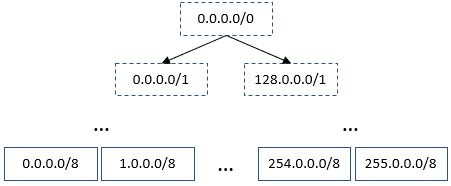
\includegraphics[width=\linewidth]{HHH/jpg_figures/init.JPG}
\caption[An example of partitioning the hierarchy given $256$ counters]{Given $C=256$ counters, the algorithm partitions the IP\_SRC hierarchy ($H=32$) at level $8$ into disjoint sets and assigns a counter per flowset.}
\label{fig:init}
\end{figure}

During each round, where packets with respective values arrive, their keys are extracted and the counter of the matching flowset is updated with the respective value. The keys of the packets depend on the flow definition the user is using, usually a single dimension of the IP addresses.
Furthermore, the respective values depend on which version of the problem we are tackling, the unweighted or the weighted version. In the unweighted version, we count the number of packets per flow, thus the values attached to each packet are 1. In the weighted version, we count the byte count of each flow, thus the values are the byte count field of the IP header.

At the end of each round, the algorithm takes a decision regarding splitting flows. This means that the algorithm exams the aggregate values of the monitored flowsets and now should filter out ``uninteresting" flowsets to allow allocating counters to finer (more specific) flowsets in order to move down the hierarchy. The most obvious candidates to refine are flowsets that had more than $\phi$ of the total frequency of the current period. However, since we refining each single flowsets into two flowsets, we have enough counter to refine the top $\frac{C}{2}$ flowsets. Thus, the algorithm sorts the monitored flowsets according to their counters values, refines the top $\frac{C}{2}$ and reassign the $C$ counter to monitor these new flowsets.

This refinement step happens $H-log_2(C)$ times until the algorithm reaches that last level of the hierarchy. Then, a bottom-up process takes place to calculate the set of candidate hierarchical heavy hitters. This process is a straightforward calculation of the conditional frequency of each previously monitored flowset and output those that exceed the threshold.

This calculation does not require any estimation of the frequencies between the rounds since the rounds are equal. This approach works extremely well if the streams are stable over time. However, fluctuations in the flow's frequencies among the rounds, might cause missing some of the HH and thus some of the HHH flows. This is, of course, the main drawback of the \simpleAlgo Algorithm.

One approach to tackle this drawback is splitting the trace into a smaller constant number of rounds (e.g. 4). This assumes, that the longer each round the more stable is the flows distribution among these rounds. This is the motivation behind the Multiple Split Algorithm presented below.

Another drawback of this algorithm is the lack of a ``reconsidering" mechanism. That is, if the algorithm does not split a given flowset in an early round it will never reconsider it, even if there is some flow in these flowsets that became later responsible for a large amount of the traffic in the trace.

\begin{algorithm}\small
    \SetKwInOut{Input}{Input}
    \SetKwInOut{Output}{Output}
    \Input{A stream of packets $S$, a threshold $\phi$, number of counters $C$ and the depth of the hierarchy $H$}
    \Output{set of hh and hhh in $S$}
    $F = init\_flowsets(C)$\;
    $number\_rounds=H+1-log_2(C)$\;
    \ForEach{$r$ in $\{1..number\_rounds\}$}
    {
        $counters=assign\_counters(F)$\;
        $packets=get\_round\_packets(r, number\_of\_rounds)$\;
        \ForEach{$counter$ in $counters$}{
            counter\_packets=$\{p\in packets : flow(p)\in counter.flow\}$\;
            counter.value=$\sum\limits_{p \in counter\_packets}value(p)$\;
        }
        \If{$r < number\_rounds$}
        {
            $top\_flowsets=sort(F, counters)[1:\frac{C}{2}]$\;
            $F=refine\_flowsets(top\_flowsets,1)$\;
        }
    }
    $hh\_per\_level=calculate\_hh\_per\_level(\phi)$\;
    $hhh\_per\_level=calculate\_hhh\_per\_level(\phi, hh\_per\_level)$\;
    return $hh\_per\_level, hhh\_per\_level$
    \SetAlgoRefName{\simpleAlgo}
    \caption{}
    \label{algo:simple_split}
\end{algorithm}

\section{The \multipleAlgo Algorithm}
The \multipleAlgo Algorithm follows that same motivation of the \simpleAlgo Algorithm, while trying to relax its stability assumptions.
In order to achieve that, we facilitate the ability to refine a given flowset not into just two disjoint flowsets, but rather into several $2^l$ disjoint flowsets.

The motivation behind this larger refinement process is that it results in smaller number of more stable rounds. The larger the round compared to the trace's size, the more we expect that it's flows distribution is closer to the entire trace distribution. Furthermore, this way we have a lower probability of  deviating from the real HH flows down the hierarchy, due to bursts of other non HH flows or fluctuations in the real HH flows.

This larger refinement process allows the algorithm to advance several levels down the hierarchy at once. Since the algorithm is still limited to $C$ counters, this comes at a cost that the algorithm can refine less flowsets than \simpleAlgo Algorithm at each round. If at a given round the algorithm advances $l$ levels, then to keep the limit of using $C$ counters, it should refine each of the top $\floor{\frac{C}{2^l}}$ flowsets into $2^l$ disjoint flowsets.

The initialization step is the same as in the \simpleAlgo Algorithm with the addition of calculating the levels step. In each step the algorithm should decide at which levels of the hierarchy to monitor. It is clear that the first level should be $\floor{log_2(C)}$ level in order to cover the entire frontier of the trie. Furthermore, the last level should be the depth of the hierarchy $H$, in order to be able to calculate the set of candidate HH and HHH correctly.

We calculate the levels to be monitored as part of the algorithm initialization. This is needed in order for the algorithm to know how many rounds of monitoring are expected so as to partition the trace into an adequate number of parts. One might consider a dynamic approach of calculating the next level ``as we go", however this approach has no clear advantage in performance and in addition it imposes a new complication. Since in such a dynamic approach not all rounds are equal, the algorithm must use estimation when calculating the conditional frequencies of suspect HHH flows, possibly as proposed in~\cite{Zhang2004}. Any such estimation step adds additional error to the final result with no clear advantage.

The rest of the algorithm is similar to the ~\simpleAlgo Algorithm, except the refining of the flowsets, which replaces each candidate flowsets into $2^l$ disjoint flowsets rather than simply two. In fact, if the calculating levels step returns all levels (starting form $log_2(C)$ up to $H$) then the algorithm converges to the ~\simpleAlgo Algorithm.

It is common to use the full byte levels ($8, 16, 24,32$ as the monitored levels~\cite{MST, BenBasat2017}.   For example, if we consider the IP\_SRC hierarchy $H=32$ with $2^{10}=1024$ counters. The initial step would be to assign the counters at level $10$ of the hierarchy. Then, at the end of the respective rounds, the algorithm will advance to levels 16, 24 and 32.
Previous works that reported HH and HHH in non 1-bit granularity limited their monitored to that specific granularity. Which means, they can not reconstruct from the non 1-bit data any insights on finer granularity HH and HHH. In the contrary, the \multipleAlgo Algorithm does not suffer from this limitation. Despite constructing the monitoring levels in non 1-bit granularity, the algorithm reconstructs the frequencies of all the inner nodes of the monitored trie.

\begin{algorithm}\small
    \SetKwInOut{Input}{Input}
    \SetKwInOut{Output}{Output}
    \Input{A stream of packets $S$, a threshold $\phi$, number of counters $C$ and the depth of the hierarchy $H$}
    \Output{set of hh and hhh in $S$}
    $F = init\_flowsets(C)$\;
    $levels=calculate\_levels(C,H)$\;
    $current\_level=levels[0]$\;
    $number\_rounds=|levels|$\;
    \ForEach{$r$ in $\{1..number\_rounds\}$}
    {
        $counters=assign\_counters(F)$\;
        $packets=get\_round\_packets(r, number\_of\_rounds)$\;
        \ForEach{$counter$ in $counters$}{
            counter\_packets=$\{p\in packets : flow(p)\in counter.flow\}$\;
            counter.value=$\sum\limits_{p \in counter\_packets}value(p)$\;
        }
        \If{$r < number\_rounds$}
        {
            $l=levels[r]-current\_level$\;
            $top\_flowsets=sort(F, counters)[1:\floor{\frac{C}{2^l}]}$\;
            $F=refine\_flowsets(top\_flowsets,l)$\;
        }
    }
    $hh\_per\_level=calculate\_hh\_per\_level(\phi)$\;
    $hhh\_per\_level=calculate\_hhh\_per\_level(\phi, hh\_per\_level)$\;
    return $hh\_per\_level, hhh\_per\_level$
    \SetAlgoRefName{\multipleAlgo}
    \caption{}
    \label{algo:multiple_split}
\end{algorithm}

\section{\ref{algo:htf} Algorithm}

One of the main drawbacks of the \simpleAlgo and \multipleAlgo Algorithm is the lack of a retracting mechanism. That is, once a flowset did not have enough frequency and was split further, we will not reconsider it again. The \ref{algo:htf} Algorithm remedies the lack of this mechanism.

We note that at the first round, the previous algorithms partition the space of flows into disjoint flowsets depending on the number of counters. At this initial step, all possible flows are covered by a single flowset. However, once a splitting decision is taken, only suspect flowsets will be partitioned and other flowset will stop being monitored. This  usually keeps a vast part of the flow space uncovered.

In order to overcome this, the \ref{algo:htf} Algorithm tries to retract up the hierarchy the part of the flowsets that previously were not be monitored. This retraction will come at a cost of not freeing those counters to measure more refined flowsets as before. Thus, the retraction should be to the highest level possible in the hierarchy.

When considering up to which point to retract these flowsets, one should consider two main aspects. The first one is retracting to the highest level while still not having a flowsets which is above the threshold.  Such flowsets are likely to split once again at the next round. The other consideration is to monitor flowsets which consist a frontier of the whole flow space and still maintain a disjoint partition.

\begin{figure}
	\centering
    \subfloat[First Round Frontier]{
        \label{subfig:first_round}{
        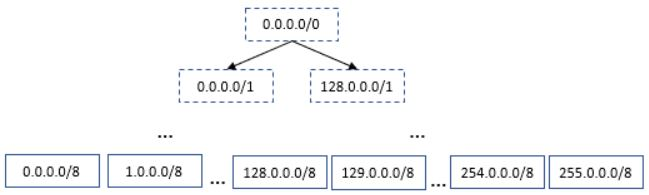
\includegraphics[width=\linewidth]{HHH/jpg_figures/retract1.JPG}
        }
    }
    \hfill
    \subfloat[Second Round Frontier] {
        \label{subfig:second_round}{
        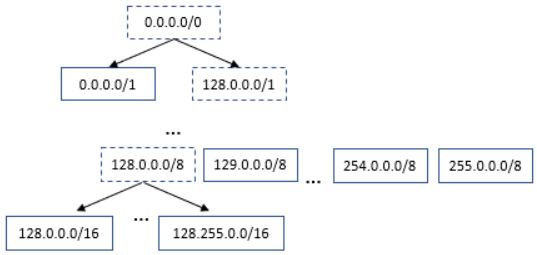
\includegraphics[width=\linewidth]{HHH/jpg_figures/retract2.JPG}
        }
    }
\caption{An example of the retraction mechanism in \ref{algo:htf} Algorithm.}
\label{fig:retract}

\end{figure}

Figure~\ref{fig:retract} depicts an example of the retraction mechanism in action for an IP\_SRC hierarchy. In this figure, the CIDR mask inside the nodes represents the flowset of this node. Furthermore, nodes with full outline are the monitored nodes, while nodes with dashed outline are non monitored nodes.

At the first round, the algorithm starts monitoring the whole flow space at level 8. As a result of the monitoring in the first round, the algorithm decided to split only the flowset $128.0.0.0/8$ because it is the only flowset that surpassed the threshold. Instead of simply abandoning the other flowsets, the algorithm tries to recursively retract to the highest level.

This recursive retracting start by classifying all flowsets at the current level into several categories: refine, keep and retract. flowsets that are classified as refine are flowsets that surpasses the threshold, these flowsets are interesting and the algorithm  partitions them in a lower level at the next round. Flowsets that are siblings of refine flowsets will be classified as keep, these flowsets did not surpass the threshold but can not be retracted to higher level since their siblings are refined. All other flowsets are classified as retract, and are aggregated into their common ancestor at a higher level.

We note that once  two siblings are classified as retract at level $l$, then their common ancestor is added at level $l-1$. When processing the level $l-1$, if this ancestor surpassed the threshold then these two siblings will be added back to the frontier at level $l$ as refine of level $l-1$.

However, when the algorithm decides on the refine set at the currently monitored level, it might partition these flowsets more than one level down the hierarchy as the case with the \multipleAlgo Algorithm, depending on the configurations.

Subfigure~\ref{subfig:second_round} depicts the frontier after the retraction process. The flowset $128.0.0.0/8$ was in the refine set of level 8 and thus was refined into the flowsets $128.0.0.0/16$ up to $128.255.0.0/16$. The flowset $129.0.0.0/8$ was classified as a keep in level 8 since its sibling was classified as a refine in the same level. The flowsets in the range of $0.0.0.0/8$-$127.0.0.0/8$ were not active during the first round, and thus were retracted up to level 1 and will be monitored by a single counter at the flowset $0.0.0.0/1$. The flowset $0.0.0.0/1$ was classified as keep at level 1 since its sibling was not present when level 1 was process, meaning it was partitioned at lower levels.

The flowsets $254.0.0.0/8, 255.0.0.0/8$ did not surpass the threshold thus were not classified as refine at level 8 and thus should be retracted, but assuming that their common ancestor $254.0.0.0/7$ did surpass the threshold and were classified as refine, they were added back to the frontier at level 8.

Up to this point we overlooked and important detail of the retracting mechanism, the affect of retracting on the number of available counters. In the best case scenario, the retracting mechanism manages to retract vast parts of the frontier to higher levels and saving enough counters, more than needed for refining flowsets at the refine set of the current level. In this scenario, the algorithm still managed to keep the frontier intact, covering the whole space, and to refine the interesting flowsets as needed.
If additional counters are available, the algorithm unretracts higher levels by refining their flowsets.

This unretacting step, happens only if we saved enough counters, and the motivation behind is to set the algorithm in better position for the next round. That is, since we have spare counters after all the required refinements, we partition flowsets at the higher position of the hierarchy into a lower level since these flowsets are the most aggregated and are the most prone to surpass the threshold without any actual child that surpasses the threshold.

On the other hand, in the worst scenario the retracting mechanism does not save enough counters to enable full refinement of the frontier. This scenario might happen in a balanced trace over the hierarchy where the algorithm does not manages to retract the frontier up to the higher levels. While the most common possibility of this scenario is that the number of counters is in the order of the number of HHH in the trace. In such scenario, the algorithm does not have enough counter for full refinement and for keeping the frontier intact since the set of suspect HH are in the order of the number of the available counters and the algorithm track each suspect HH by a single counter at each point.

The complexity of the retracting and unretracting step of this algorithm is still $O(HC)$, since at most we perform recursive retraction over $(H)$ levels and unretracting over the same $O(H)$ levels. The most important thing to note when considering the complexity, is that at any given level we perform at most $O(C)$ operation and not $O(2^l)$ operations, since  at each level the algorithm monitors at most $O(C)$ flowsets and when performing the classification of each level we consider only monitored flowsets.

Thus, despite complicating the per round operation the algorithm still performs a constant per-packet operation and a constant number of times a  heavier operation that is still linear in the number of counters and $O(1)$ when considering the number of packets or even the number of active flows.
\begin{algorithm}\small
    \SetKwInOut{Input}{Input}
    \SetKwInOut{Output}{Output}
    \Input{A stream of packets $S$, a threshold $\phi$, number of counters $C$ and the depth of the hierarchy $H$}
    \Output{set of HH and HHH in $S$}
    $F = init\_flowsets(C)$\;
    $levels=calculate\_levels(C,H)$\;
    $current\_level=levels[0]$\;
    $number\_rounds=|levels|$\;
    \ForEach{$r$ in $\{1..number\_rounds\}$}
    {
        $counters=assign\_counters(F)$\;
        $P=get\_round\_packets(r, number\_of\_rounds)$\;
        \ForEach{$counter$ in $counters$}{
            counter.value=$\sum\limits_{\{p\in P : flow(p)\in counter.flowset\}}value(p)$\;
        }
        \If{$r < number\_rounds$}
        {
            $l=levels[r]-current\_level$\;
            $to\_refine, retracted = retract\_frontier(counters, F, current\_level)$\;
            $refined = refine\_flowsets(to\_refine,l)$\;
            $needed\_counters = |refined \cup retraced|$\;
            \If{$needed\_counters > C$}{
                $abort()$\;
            }
            \Else{
                $retracted = unretract\_frontier(C - needed\_counters, retracted)$\;
            }
            $F=refined \cup retracted$\;
        }
    }
    return $calculate\_hhh\_bottom\_up(\phi)$\; 
    \ignore{
    $hh\_per\_level=calculate\_hh\_per\_level(\phi)$\;
    $hhh\_per\_level=calculate\_hhh\_per\_level(\phi, hh\_per\_level)$\;
    return $hh\_per\_level, hhh\_per\_level$\;
    }
    \SetAlgoRefName{\htfAlgo}
    \caption{}
    \label{algo:htf}
    \vspace{-0.1cm}
\end{algorithm}

\section{\ref{algo:sa} Algorithm}

One of the main limitations of the \ref{algo:htf} Algorithm is that when the number of counters is in the same order as the number of HH flows, even after retracting the frontier, the algorithm can not fully refine the suspect flowsets. In order to explain how to overcome this limitation, we examine the state of the frontier when a retraction happens in a sub-trie with a single refine flowset.

Figure~\ref{fig:sa_vs_htf} represents the frontier after retracting and refining when the flowset $128.0.0.0/8$ was the only active flow of this sub-trie and surpassed the threshold. Since it surpassed the threshold, it was refined into the flowset in the range $128.0.0.0/16$ up to $128.255.0.0/16$. Since it was the only flowset that surpassed the threshold, the retraction step tries to free counters however it keeps a path from the highest root that did not surpass the threshold down to the interesting flowset. This ``wastes" several counters in the following round. None of the flowsets $129.0.0.0/8, 130.0.0./7, ..., 192.0.0.0/2$ could be retracted more since their siblings are not present in the respective level, even if they had 0 frequency in the round.

The \ref{algo:sa} Algorithm tries to save counters by replacing the allocation for these non-interesting flowsets with a single counter on their common ancestor. this breaks the promise to keep a disjoint partition of the frontier. Instead of allocating a counter per level, the algorithm allocates a counter to the highest shared ancestor that did not surpass the threshold. This shared ancestor counts the traffic all of its sub-trie and then we subtract the ``interesting" flowsets for which we have separate counters.

The ellipses node in Figure~\ref{fig:sa_vs_htf} represents this shared ancestor and the monitored flowsets in the example are $128.0.0.0/1$ and all of the flowsets at level 16. If we compare this to the monitored set in ~\ref{algo:htf} Algorithm, that consists of the solid outline nodes, it requires $7$ fewer counters. While these savings seem low, they might happen at any level of the hierarchy and in any part of the flow space, with a compound effect of freeing enough counters to make the algorithm deployable even with a small number of counters.

One must note that in this algorithm, flowsets from various levels are monitored together and one must be very careful when comparing their frequencies since they set of flows from different sizes. One might be tempted to normalize the frequencies of the larger flowsets in order to be able to compare them to the smaller flowsets and use the same flowset, but in fact, this might turn to be counter constructive.

The main motivation behind keeping a frontier is the ability to retract to abandoned flows, however, if we normalize the frequencies of large flowsets by dividing them by the number of flows in that flowset, then this flowset will surpass the threshold if and only if most of its flows exceed the threshold. Usually, this means that this ancestor flowset will never be refined again, missing the point of retracting into abandoned flows. Details regarding the actual steps of the algorithm are provided in Algorithm \ref{algo:sa}.

\begin{figure}
	\centering
	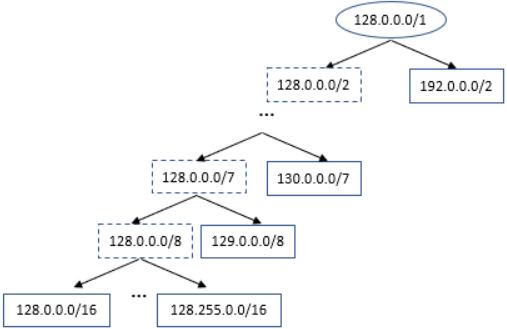
\includegraphics[width=\linewidth]{HHH/jpg_figures/sa_vs_htf.JPG}
\caption[An example of a frontier after retraction in \ref{algo:htf} and \ref{algo:sa} algorithms]{The frontier after retraction in \ref{algo:htf} and \ref{algo:sa} with a single interesting flowset.}
\label{fig:sa_vs_htf}
\end{figure}

\begin{algorithm}\small
    \SetKwInOut{Input}{Input}
    \SetKwInOut{Output}{Output}
    \Input{A stream of packets $S$, a threshold $\phi$, number of counters $C$ and the depth of the hierarchy $H$}
    \Output{set of HH and HHH in $S$}
    $F = init\_flowsets(C)$\;
    $levels=calculate\_levels(C,H)$\;
    $current\_level=levels[0]$\;
    $number\_rounds=|levels|$\;
    \ForEach{$r$ in $\{1..number\_rounds\}$}
    {
        $counters=assign\_counters(F)$\;
        $P=get\_round\_packets(r, number\_of\_rounds)$\;
        \ForEach{$counter$ in $counters$}{
            counter.value=$\sum\limits_{\{p\in P : flow(p)\in counter.flowset\}}value(p)$\;
        }
        \If{$r < number\_rounds$}
        {
            $l=levels[r]-current\_level$\;
            $to\_refine = calculate\_to\_refine(counters, F, current\_level)$\;
            $refined = refine\_flowsets(to\_refine,l)$\;
            $ancestors = \{\}$\;
            \ForEach{$f$ in $refined$}{
                $sa=calculate\_shared\_ancestor(f, F)$\;
                $ancestors.add(sa)$\;
            }
            $F=refined \cup ancestors$\;
        }
    }
    return $calculate\_hhh\_bottom\_up(\phi)$\; 
    \ignore{
    $hh\_per\_level=calculate\_hh\_per\_level(\phi)$\;
    $hhh\_per\_level=calculate\_hhh\_per\_level(\phi, hh\_per\_level)$\;
    return $hh\_per\_level, hhh\_per\_level$\;
    }
    \SetAlgoRefName{\saAlgo}
    \caption{}
    \label{algo:sa}
    \vspace{-0.1cm}
\end{algorithm}
\section{Evaluation}
We evaluated our algorithms using the following real life traces: (1) CAIDA'16: CAIDA Internet Traces from ``Equinix-Chicago'' in 2016~\cite{CAIDA2016}, (2) CAIDA'18: CAIDA Internet Traces from ``Equinix-NewYork'' in 2018~\cite{CAIDA2018}. We considered IP source hierarchies in a single bit granularities, such hierarchies were also used in~\cite{ben2017constant, SpaceSaving}, and considered the unweighted frequencies of items (i.e., the number of packets). Each data point is the average of 10 runs, where each run started from a randomly selected point in the given trace.

We use the \textit{Recall} and \textit{Precision} metrics proposed in ~\cite{ffMetrics} to evaluate the performance of the suggested algorithms. In order to compute these metrics, we calculated the true set of HH and HHH using a space intensive algorithm that allocates a counter per flow for exact measurements.
Recall is the number of true HHHs detected by the algorithm divided by the number of true HHHs. This metric is equivalent to the Detection Rate of the algorithm, i.e., what is the percentage of HHHs the algorithm detects.
Precision is the number of true HHHs detected by the algorithm divided by the number of reported suspect HHH. This metric complements the false positive rate of the algorithm and tries to grasp how many of the suspect HHHs the algorithm was mistaken.

We denote our proposed algorithms with ``SS" for \simpleAlgo, ``MS" for \multipleAlgo, ``HTF" for \ref{algo:htf} and ``SA" for \ref{algo:sa}. Furthermore, we use ``RHHH" to denote the algorithm proposed in~\cite{ben2017constant} and ``MST" to denote the algorithm proposed in~\cite{SpaceSaving}. These algorithms solve an approximate version of the problem with an accuracy parameter $\epsilon$, when comparing with them we expand the set of true HHH by a slack of $\epsilon T$.

\begin{figure}
    \centering
    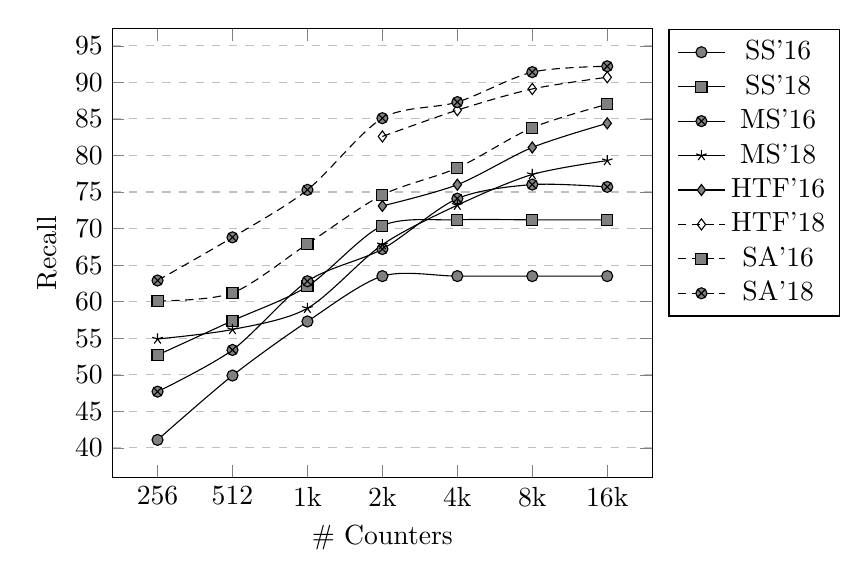
\begin{tikzpicture}
        \begin{axis}[
        xlabel={\# Counters},
        ylabel={Recall},
        xtick=data,
        xticklabels={256, 512, 1k, 2k, 4k, 8k, 16k},
        ytick={0,5,10,15,20,25,30,35,40,45,50,55,60,65,70,75,80,85,90,95,100},
        % legend pos=south east,
        % legend columns=2,
        ymajorgrids=true,
        grid style=dashed,
        legend style ={ at={(1.03,1)}, 
        anchor=north west, draw=black, 
        fill=white,align=left},
        cycle list name=black white,
        smooth
        ]
            \addplot
            coordinates {
                (1,41.1)(2,49.9)(3,57.3)(4,63.5)(5,63.5)(6,63.5)(7,63.5)
            };
            \addlegendentry{SS'16};
            \addplot
            coordinates {
                (1,52.7)(2,57.4)(3,62.1)(4,70.4)(5,71.2)(6,71.2)(7,71.2)
            };
            \addlegendentry{SS'18};
            \addplot
            coordinates {
                (1,47.7)(2,53.4)(3,62.8)(4,67.2)(5,74.1)(6,76.02)(7,75.7)
            };
            \addlegendentry{MS'16};
            \addplot
            coordinates {
                (1,54.9)(2,56.2)(3,59.1)(4,67.8)(5,73.2)(6,77.4)(7,79.3)
            };
            \addlegendentry{MS'18};
            \addplot
            coordinates {
                (4,73.1)(5,76.0)(6,81.1)(7,84.4)
            };
            \addlegendentry{HTF'16};
            \addplot+[black, mark=diamond]
            coordinates {
                (4,82.6)(5,86.2)(6,89.1)(7,90.7)
            };
            \addlegendentry{HTF'18};
            \addplot
            coordinates {
                (1,60.1)(2,61.2)(3,67.9)(4,74.6)(5,78.3)(6,83.8)(7,87.0)
            };
            \addlegendentry{SA'16};
            \addplot
            coordinates {
              (1,62.9)(2,68.8)(3,75.3)(4,85.1)(5,87.3)(6,91.4)(7,92.2)
            };
            \addlegendentry{SA'18};
        \end{axis}
    \end{tikzpicture}
    \caption{The Recall of the algorithms for various number of counters on CAIDA'16 and CAIDA'18 traces.}
    \label{fig:recall}
\end{figure}

Figure~\ref{fig:recall} shows the \textit{Recall} of the various algorithms as a function of the number of available counters. Each line describes a single algorithm and the CAIDA trace, the runs are on random parts of the trace of $2^{25}$ packets (about one minute of traffic) with threshold $\phi=0.001$. It is worthy to note that the performance on CAIDA'18 trace is usually better than those of CAIDA'16 trace, this is since in CAIDA'16 trace the heaviest flows are not as stable as in CAIDA'18. Also, note that the number of HH in these traces at a given level of the hierarchy is at most 200. This explains the overall poor performance when using fewer counters than 512.

When considering the Recall of ~\simpleAlgo and ~\multipleAlgo algorithms, one can notice an improvement as the number of counters increases up to a point where adding more counters does not help anymore. This limitation is explained by the lack of a retracting mechanism in these algorithms, thus missing a portion of the HHH that starts late in the monitoring interval and more specifically after the first round.

The ~\ref{algo:htf} Algorithm can not run properly for a very low number of counters, that is up to $1k$ counters. That is due to the fact that sometimes the attempt to retract the frontier does not free enough counters to perform full refinement of the interesting flowsets. Thus, we did not report the results for the number of counters where at least one run of the algorithm did not finish due to this reason. For a higher number of counters (starting from $2k$) the algorithm manages to breach the observed limitation at ~\simpleAlgo and ~\multipleAlgo algorithms due to its retracting mechanism.

The main advantage of ~\ref{algo:sa} algorithm compared to ~\ref{algo:htf} algorithm lies in the ability to deploy it using a smaller number of counters. The difference in the recall of the algorithms is not statistically significant, where both reach around 90\% recall on the CAIDA'18 traces.

\begin{figure}
    \centering
    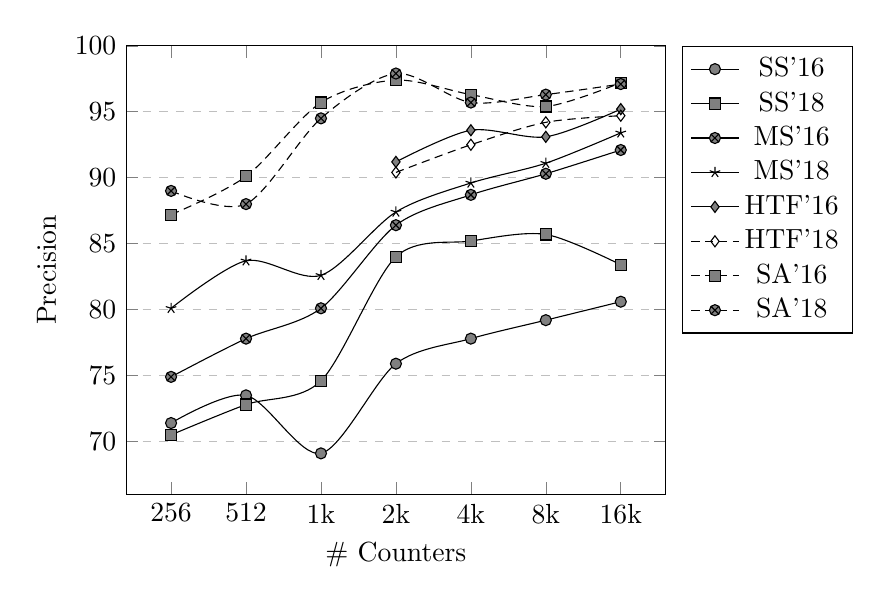
\begin{tikzpicture}
        \begin{axis}[
        xlabel={\# Counters},
        ylabel={Precision},
        xtick=data,
        xticklabels={256, 512, 1k, 2k, 4k, 8k, 16k},
        ytick={0,5,10,15,20,25,30,35,40,45,50,55,60,65,70,75,80,85,90,95,100},
        % legend pos=south east,
        % legend columns=2,
        ymajorgrids=true,
        ymax=100,
        grid style=dashed,
        legend style ={ at={(1.03,1)}, 
        anchor=north west, draw=black, 
        fill=white,align=left},
        cycle list name=black white,
        smooth
        ]
            \addplot
            coordinates {
                (1,71.4)(2,73.5)(3,69.1)(4,75.9)(5,77.8)(6,79.2)(7,80.6)
            };
            \addlegendentry{SS'16};
            \addplot
            coordinates {
                (1,70.5)(2,72.8)(3,74.6)(4,84.0)(5,85.2)(6,85.7)(7,83.4)
            };
            \addlegendentry{SS'18};
            \addplot
            coordinates {
                (1,74.9)(2,77.8)(3,80.1)(4,86.4)(5,88.7)(6,90.3)(7,92.1)
            };
            \addlegendentry{MS'16};
            \addplot
            coordinates {
                (1,80.1)(2,83.7)(3,82.6)(4,87.4)(5,89.6)(6,91.1)(7,93.4)
            };
            \addlegendentry{MS'18};
            \addplot
            coordinates {
                (4,91.2)(5,93.6)(6,93.1)(7,95.2)
            };
            \addlegendentry{HTF'16};
            \addplot+[black, mark=diamond]
            coordinates {
                (4,90.4)(5,92.5)(6,94.2)(7,94.7)
            };
            \addlegendentry{HTF'18};
            \addplot
            coordinates {
                (1,87.2)(2,90.1)(3,95.7)(4,97.4)(5,96.3)(6,95.4)(7,97.2)
            };
            \addlegendentry{SA'16};
            \addplot
            coordinates {
                (1,89.0)(2,88.0)(3,94.5)(4,97.9)(5,95.7)(6,96.3)(7,97.1)
            };
            \addlegendentry{SA'18};
        \end{axis}
    \end{tikzpicture}
    \caption{The Precision of the algorithms for various number of counters on CAIDA'16 and CAIDA'18 traces.}
    \label{fig:precision}
\end{figure}

Figure~\ref{fig:precision} depicts the \textit{Precision} of the various algorithms as a function of the number of available counters in the same settings as Figure~\ref{fig:recall}. More specifically, the figure shows how many flows reported by the algorithm as HHH were actually a true HHH, i.e., how precise was the algorithm in its reports. All of our algorithms tend to report most of their false positives, reported flows that are not HHH, in the higher levels of the hierarchy. Due to the parts of the hierarchy that are not monitored but still see some traffic, however, in lower levels the algorithms have a better estimation of the flow's frequencies and whether they are HHH or not. Furthermore, the higher in the hierarchy the calculation of HHH happens, the more it is prone to errors due to errors in the lower levels.

We note that the difference in precision between the two traces in a given algorithm is not that noticeable. This is explained by the fact that if even in CAIDA'16 the heaviest flows are not consistent compared to CAIDA'18, the algorithms manage to filter out flows that lead to splitting at higher levels but did not remain suspect HH throughout the rounds.

Furthermore, the trend of better performance with more counter we observed in Figure~\ref{fig:recall} is less clear especially in ~\simpleAlgo and ~\multipleAlgo algorithms. That is, sometimes more counters lead to a small decrease in the precision of the algorithms. This might be explained by the fact that with more counters these simple algorithms focus on more unimportant parts down the hierarchy.

The precision of ~\ref{algo:sa} Algorithm reaches more than 95\% for $1k$ counters and even around 97\% for more than that. This means, that given enough counters this algorithm detects around 90\% of the true HHH and reports no more than 3\% non-HHH flows. For the same reasons mentioned before, the results of ~\ref{algo:htf} Algorithm were not reported for counters less than $2k$.

\begin{figure}
    \centering
    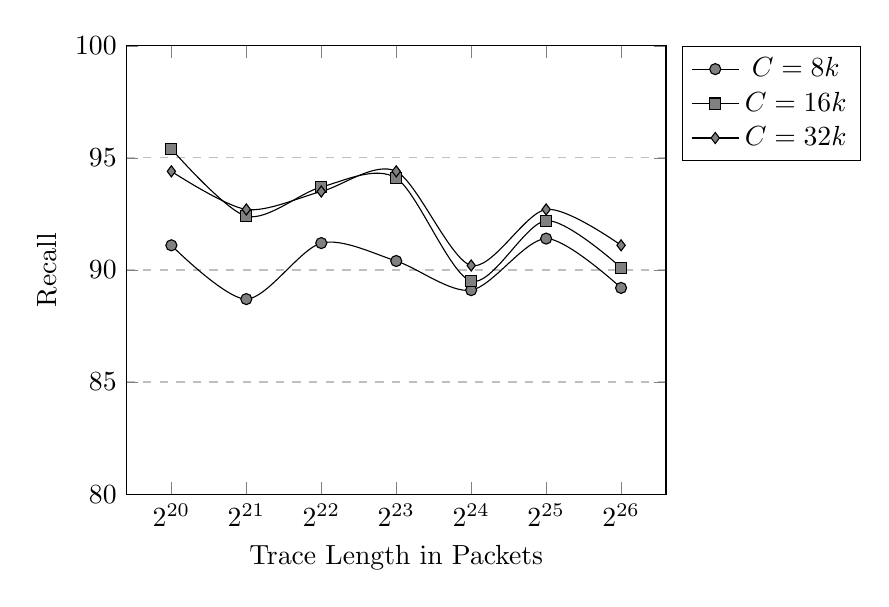
\begin{tikzpicture}
        \begin{axis}[
        xlabel={Trace Length in Packets},
        ylabel={Recall},
        xtick=data,
        xticklabels={$2^{20}$, $2^{21}$, $2^{22}$, $2^{23}$, $2^{24}$, $2^{25}$, $2^{26}$},
        ytick={0,5,10,15,20,25,30,35,40,45,50,55,60,65,70,75,80,85,90,95,100},
        % legend pos=south east,
        % legend columns=2,
        ymajorgrids=true,
        ymax=100,
        ymin=80,
        grid style=dashed,
        legend style ={ at={(1.03,1)}, 
        anchor=north west, draw=black, 
        fill=white,align=left},
        cycle list name=black white,
        smooth
        ]
            \addplot
            coordinates {
                (1,91.1)(2,88.7)(3,91.2)(4,90.4)(5,89.1)(6,91.4)(7,89.2)
            };
            \addlegendentry{$C=8k$};
            \addplot
            coordinates {
                (1,95.4)(2,92.4)(3,93.7)(4,94.1)(5,89.5)(6,92.2)(7,90.1)
            };
            \addlegendentry{$C=16k$};
            \pgfplotsset{cycle list shift=2}
            \addplot
            coordinates {
                (1,94.4)(2,92.7)(3,93.5)(4,94.4)(5,90.2)(6,92.7)(7,91.1)
            };
            \addlegendentry{$C=32k$};
        \end{axis}
    \end{tikzpicture}
    \caption[Recall of ~\ref{algo:sa} Algorithm as function of the trace length]{The recall of~\ref{algo:sa} Algorithm for various length of trace on CAIDA'18.}
    \label{fig:trace_length}
\end{figure}

Figure~\ref{fig:trace_length} depicts the recall of ~\ref{algo:sa} Algorithm (under the same settings) as a function of the trace length (number of packets processed) for a given number of counters. It easy to see that the algorithm does not require any convergence period in order to achieve high recall. Furthermore, there is no consistent trend in the recall of the algorithm as a function of the trace length, besides slight variations that can be explained as fluctuations in the different parts of the trace.

\begin{figure}
    \centering
    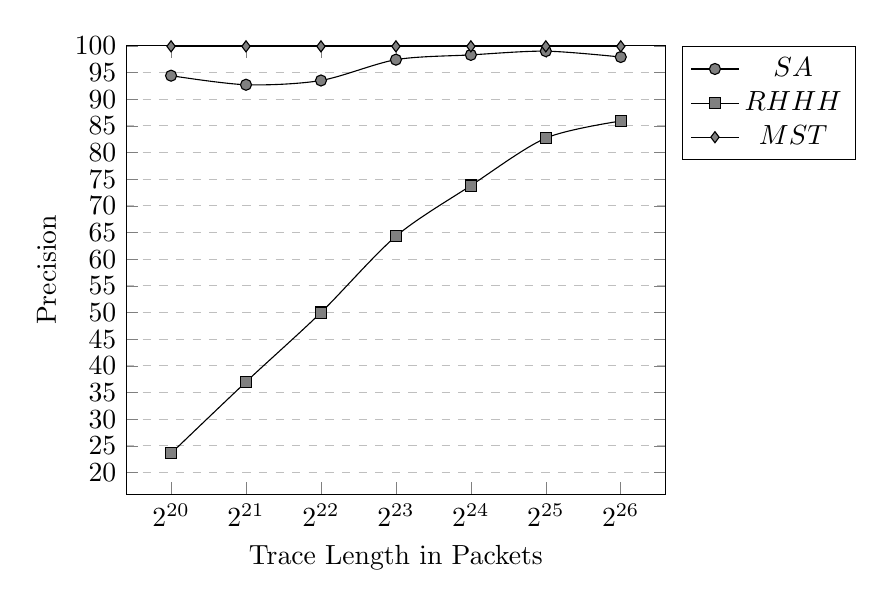
\begin{tikzpicture}
        \begin{axis}[
        xlabel={Trace Length in Packets},
        ylabel={Precision},
        xtick=data,
        xticklabels={$2^{20}$, $2^{21}$, $2^{22}$, $2^{23}$, $2^{24}$, $2^{25}$, $2^{26}$},
        ytick={0,5,10,15,20,25,30,35,40,45,50,55,60,65,70,75,80,85,90,95,100},
        % legend pos=south east,
        % legend columns=2,
        ymajorgrids=true,
        ymax=100,
        grid style=dashed,
        legend style ={ at={(1.03,1)}, 
        anchor=north west, draw=black, 
        fill=white,align=left},
        cycle list name=black white,
        smooth
        ]
            \addplot
            coordinates {
                (1,94.4)(2,92.7)(3,93.5)(4,97.4)(5,98.3)(6,99.0)(7,97.9)
            };
            \addlegendentry{$SA$};
            \addplot
            coordinates {
                (1,23.6)(2,37.0)(3,50.0)(4,64.3)(5,73.8)(6,82.7)(7,85.9)
            };
            \addlegendentry{$RHHH$};
            \pgfplotsset{cycle list shift=2}
            \addplot
            coordinates {
                (1,99.9)(2,99.9)(3,99.9)(4,99.9)(5,99.9)(6,99.9)(7,99.9)
            };
            \addlegendentry{$MST$};
        \end{axis}
    \end{tikzpicture}
    \caption{The precision of ~\ref{algo:sa} Algorithm compared to ``MST" and ``RHHH" on CAIDA'16 trace, for $\phi=0.01, \epsilon=0.001, C=\frac{H}{\epsilon}=\frac{32}{0.001}=32k$ on single bit IP source hierarchy for various lengths the trace.}
    \label{fig:trace_length_precision}
\end{figure}




Figure~\ref{fig:trace_length_precision} depicts the precision of the ~\ref{algo:sa} algorithm as function of the trace length (number of packets processed) compared to ``MST" and ``RHHH". As expected, ``RHHH" suffers from a convergence interval, only then it starts to keep its probabilistic guarantees of low false positive. ``MST", which requires $O(H)$ update time per-packet, achieves almost perfect precision (no false positive) as guaranteed by $\epsilon$. Our ~\ref{algo:sa} algorithm achieves a high precision rate averaged around 95\% regardless of the trace's length while holding $O(1)$ per-packet update time. The algorithms converge similarly on CAIDA`18 traces.

\section{Conclusions}
In this paper we presented several practical algorithms for  Hierarchical Heavy Hitters detection.  These algorithms can be deployed on off-the-shelf network nodes (or software devices) and can operate in line speed due to their $O(1)$ per-packet operation. The current state of the art algorithms, either require $O(H)$ per-packet operation that makes them unfeasible to be deployed in line rate or requires a convergence interval before reporting satisfactory results which makes them less relevant in many practical settings. In contrary, our algorithms perform in line-speed with $O(1)$ update per-packet without requiring any convergence interval. Furthermore, no complex data structures are needed and our algorithms only require using built-in fast counters available in any network node.

We evaluated the algorithms on two recent real Internet packets traces and showed that they yield a comparable results to the state of the art without their limitations. The evaluation showed that the best algorithm can detect up to 90\% of the HHH in a trace and report no more than 5\% non HHH flows.

These algorithms could be easily extend to the case of multi-dimensional HHH while keeping the depth of the hierarchy linear in the number of dimensions without modifying the $O(1)$ update time. Also, they allow practical detection of the weighted set of HHH flows with minimal modification of the update operations while keeping all of the algorithms promises.
In future work, we plan to study the control mechanism of the algorithms and their fine deployment issues. Furthermore, we plan to adjust the algorithms to detect DDoS attacks by facilitating the already needed calculation of HH at the lower level of the hierarchy.


\chapter{On the Practical Detection of Heavy Hitter Flows}
\section{abstract}
The detection of of Heavy Hitter (HH) flows in a network device is a critical building block in many control and management tasks.  A flow is considered a Heavy Hitter flow if its portion from the total traffic surpasses a given threshold.  One of the most important aspect of this detection is its practicality; i.e., being able to work in line rate using the available scarce local memory in the device.  

In this paper, we present a practical heavy hitters detection algorithm that requires a constant amount of memory (not related to the number of flows or the number of packets) and performs at most $O(1)$ operation per packet to keep with line rate speed. We present an analysis of errors for our algorithm and compare it to state-of-the-art monitoring solutions, showing a superior performance where the allocated memory is less than $1MB$. In particular, we are able to detect more HH flows with less false positive without increasing the per-packet processing time.
\section{Introduction}
\label{sec:introduction}

%\subsection{Background}
Modern Infrastructure as a Service (IaaS) providers rely on various network protocols to provide efficient service management abilities. These protocols, as well, rely heavily on the ability to provide correct and efficient network monitoring that generate the needed statistics. Such protocols belong to various service management sub-domains such as traffic engineering~\cite{microte}, anomaly detection~\cite{Moraney2016}, load balancing~\cite{networkLB}, NFV placements~\cite{NFV-dor} and many more.

The ability to provide accurate per flow statistics, while greatly important for service management protocols, is often impractical due to the high number of active flows and the limited on-chip memory needed to keep such counters. Furthermore, no remediation is expected in the near future; more flows are flowing through networks than before, line rate is ever increasing requiring counters with more width and more monitoring applications are running, requiring their own portion of the available memory. 

Given these limitations, it is important to consider designing and implementing efficient practical algorithms for various monitoring tasks~\cite{moraney2018, moraney2020}. We consider an algorithm to be an efficient practical monitoring algorithm if (1) it provides important monitoring data, (2) performs $O(1)$ operations per packet to cope with line rate, (3) uses a constant limited amount of memory that is much smaller than and not related to the number of active flows, and finally (4) implementable on memory schemes of off-the-shelf network gear.

Many of the current state-of-the-art and most notable monitoring schemes, require a non-constant amount of memory depending either on the traces size or in inverse relation to the guaranteed accuracy~\cite{slidingHH,metwally2005efficient,SpaceSaving,Ben-Basat2017}. In such schemes, the required memory is usually of size $o(\frac{1}{\epsilon})$ where $\epsilon$ is the guaranteed accuracy. This notation  hides the fact that in many practical use-cases their memory requirement is  higher than what is available in the network device.

With the increasing amount of various monitoring applications running concurrently on network devices, the approach of setting accuracy parameters per application and only then count for their required memory is not operational. This approach makes it hard for network operators to meet the memory constraint by prioritizing applications and optimizing their accuracy parameters. The correct approach to manage on-device monitoring applications is to set hard constraints on their memory footprint and only then set the desired accuracy parameters while slightly compromise the quality of the monitoring results according to the available resources. 

The quality of the monitoring results is commonly measured via two metrics, \textit{Recall} and \textit{False Positive Rate} (FPR). Recall (sometimes called also Detection Rate) measures the proportion of positives items that are correctly identified while the FPR measures the proportion of the none-positive items that are reported as positive (i,e,. misidentified) from the set of reported items.  Describing the quality of the monitoring data without reporting both metrics is not complete. Since, while high recall algorithms are preferred, this should not come at a a price of a very high FPR. An extreme example of such algorithm is the one that reports all flows as positive, this algorithm will have a recall of $100\%$ but also almost a $100\%$ FPR hindering its output useless.

Having on-device monitoring algorithms that support line rate is of high importance, no network operator in right mind would consider reducing network capacity due to the deployment of monitoring algorithms on devices. The guarantee of line rate performance usually manifests in having $O(1)$ operations per packet, the motivation is if the algorithm performs only ``light weight" operation per arriving packet it would meet the line rate requirement.

Many monitoring algorithms maintain complex schemes and data structures that require once in a while perform a ``heavy" operation (for example a re-ordering of the data scheme). Algorithms of this type claim to support line rate while having an amortized $O(1)$ operation by proving that this ``heavy" operation happens once in many packets and when its cost is split among all the relevant packets it would add a constant negligible effect.

This point of view on line rate operation is in many cases impractical. While truly it is an amortized $O(1)$ operation, during such operations, arriving packets must be stored to be later processed and this could affect the devices available buffers and affects its performance. Thus, one of our motivations is to design a scheme that performs worst-case $O(1)$ operation.

\subsection{Related Work}

While the problem of detecting Heavy Hitter Flows, is a classical monitoring problem that is easily solvable given enough memory and had been addressed heavily in the literature~\cite{fang1999computing,gilbert2001surfing,karp2003simple,Demaine2002,slidingHH,basat2017optimal,zadnik2011evolution}, little thought was given on the practicality of the deployment of the proposed solutions.

The state-of-the-art algorithm to detect HH flows was introduced in~\cite{basat2017optimal}. In this paper the authors introduced ,IM-SUM, an algorithm which solves an $\epsilon$-approximation of the \textit{frequency estimation} problem and a $(\phi, \epsilon)$-approximation of the the HH problem. The algorithm holds two monitoring tables, a passive and an active tables, then periodically replaces their roles. The motivation is that the passive table holds the ``biggest" flows and the active holds the most ``recent" flows. When the passive table gets full a ``heavy" maintenance operation is performed, that calculates the $\lfloor\frac{1}{\epsilon}\rfloor^{th}$ largest value in the passive table, drops all entries smaller than it and moves larger entries to the active table. Furthermore, a variable $q$ holds the value of the last calculated $\lfloor\frac{1}{\epsilon}\rfloor^{th}$ largest value and it functions as the estimation of flows not in any of the tables.

The main drawbacks of this algorithm are: (1) it performs a ``heavy" maintenance operation that makes its performance an amortized $O(1)$ operation, (2) it requires an amount of memory that is proportional to the inverse of the accuracy parameter $O(\frac{1}{\epsilon})$ and (3) its approximation is of the form $N(\phi -\epsilon)$ where $N$ is the number of packets, $\phi$ is the threshold and $\epsilon$ is the accuracy parameter. This means that slack given to the approximation is $\epsilon N$ which is proportional to the amount of traffic processed by the algorithm.

In~\cite{CEDAR}, the authors introduced the \textit{CEDAR} algorithm that decouples the stored flows identifiers from their estimation values by using a constant size table to store shared estimators. The algorithm holds two tables, the first one have an entry per each flow which holds the flow's identifier and an integer. This integer as an index to the second table pointing to the flow's current estimation value. Thus, the second table is a shared estimators table, where estimators values are constructed in a manner to provide unbiased estimations while achieving minimal maximal relative estimation error. When a new flow arrives, it enters the flows table with an index of $0$, meaning its initial estimation is $v_0=0$. On each arrival of a packet from a previously seen flow, the algorithm extracts its current estimation, $v_i$, and the value of the next estimator $v_{i+1}$ and increases the estimation of the flow to be $v_{i+1}$ with probability $\frac{1}{v_{i+1}-v_{i}}$.

\subsection{This paper}
The main drawback of ~\cite{CEDAR} is that it maintains an entry per each active flow in the system and thus unpractical as a HH algorithm.
In this paper, we devise an algorithm that takes benefit of the constant amount of estimators in the CEDAR algorithm while keeping the needed memory also constant. This can be achieved since we only care about the size of large flows (HH candidate) and we do not need to maintain an estimator for each small flow. The main difficulty is thus identifying the flows that need to be monitored; this is done by looking at flows that have frequent appearance.  We keep in a table called   \sfa\ all recent flows, and when a new packet from one of these flows arrives before the flow is evicted from the table we mark this flow as a HH candidate and advance it to the \cs\ where its frequency is being measured by the shared estimators. 

The main contribution of this paper is that we present a practical heavy hitters detection algorithm that requires a constant amount of memory (not related to the number of flows or the number of packets) and performs at most $O(1)$ operation per packet to keep with line rate speed. Furthermore, we compare it to state-of-the-art monitoring solutions on real internet traces, showing a superior performance where the allocated memory is less than $1MB$.


In Section~\ref{sec:architecture} we describe the architecture and the data structures of our algorithm, the \cs\ algorithm, and then in Section~\ref{sec:theory}, we analyze  the possible source of errors. In Section~\ref{sec:improvemnts} we present a less robust variant of our algorithm, the \eb\ algorithm, that performs better when the trace is heavy tailed. Then in Section~\ref{sec:evaluation} we evaluate the \cs\ algorithm performances and compare it to state-of-art-algorithm, and finally we conclude in Section~\ref{sec:conclusions}.

\section{The \cs\ Algorithm}
\label{sec:architecture}
%\subsection{Data Structures}
The \cs\ algorithm is based on three data structure: (1) the \textit{\sfa}, (2) the \textit{\cs}, and (3) the \textit{\sea}. Figure~\ref{fig:ds} illustrates these data structures.
The algorithm uses the first two to store identifiers of flows suspected as HH flows with different levels of confidence.
In the \sfa\ the algorithm stores identifiers of flows that were recently encountered in order to track their potential growth. When this growth is fulfilled these flows are propagated to the \cs. In the \cs\ the algorithm stores identifiers of ``heavy" flows, i.e., flows that already showed some evidence for a large amount of traffic.

\begin{figure}
  \centering
  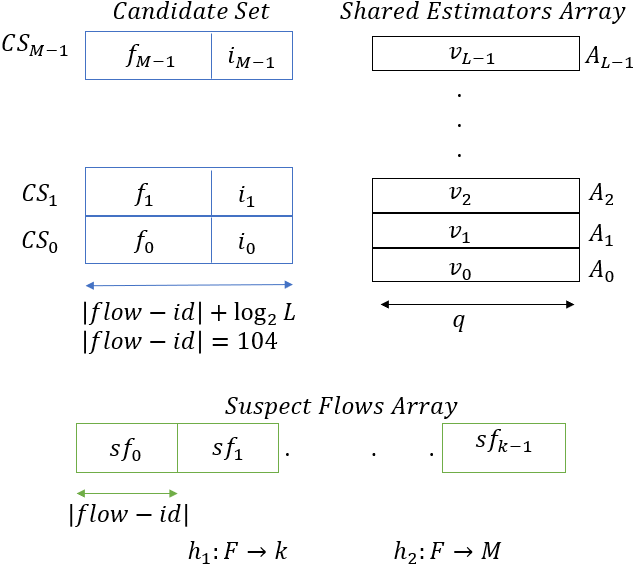
\includegraphics[width=\linewidth]{HH/figures/ds.png}
  \caption{The basic architecture of the \cs\ algorithm}
  \label{fig:ds}
\end{figure}

This way, the algorithm facilities tracking ``recent" and ``heavy" flows to estimate their frequency using the \sea. Next, we describe how a HH flow is handled by the algorithm. First, it is added into the \sfa. Then, on the second arrival of its packets, if it was not evicted in the meantime, it is propagated to the \cs. Afterward, it is tracked in the \cs\ and its frequency is estimated via the \sea.

Non HH flows that are of a negligible size usually reaches only the \sfa\ and are not propagated to the \cs. That is, until a second packet from the flow arrives, many other packets from other flows were already processed and probably have evicted the entry of the original flow from the \sfa. This way, the second arrival of a packet from this flow is considered as a new flow, since the algorithm has no data about this flow, and it will be kept at most in the \sfa\ or even not remembered by the algorithm at all.

Other non HH flows that are not negligible but still are not HH could propagate to the \cs\ from the \sfa. However, it is not enough to propagate to the \cs\ in order to be considered as a HH. A flow size estimation in the \sea\ needs to be above the threshold. The \sea\ mechanism is based on the estimation table introduced in the CEDAR algorithm~\cite{CEDAR} and it guarantees a maximal relative error of $\delta$ for any flow in the \cs, thus our algorithm might produce a false positive only on flows with frequencies in the range$[(1-\delta)\phi N, \phi N]$.

\begin{table}
\caption{A summary of the used notations}
\begin{center}
\begin{tabular}{|c|c|}
\hline
\textbf{Symbol}& \textbf{Meaning}\\
\hline
$m$& total available memory\\
\hline
$m_{CS}$& share of \cs\ memory out of $m$\\
\hline
$m_{SFA}$& share of \sfa\ memory out of $m$\\
\hline
$m_{SEA}$& share of \sea\ memory out of $m$\\
\hline
$\phi$& heavy hitter threshold\\
\hline
$N$& number of packets\\
\hline
$F$& 5-tuple flows Universe\\
\hline
$\delta$& guaranteed relative error\\
\hline
$A_i$& $i^{th}$ shared estimator\\
\hline
$L$& number of shared estimators\\
\hline
$q$& width of an estimator\\
\hline
$v_0$& the minimal estimator\\
\hline
$v$& the "propagation" parameter\\
\hline
$M$& the number of entries in the \cs\\
\hline
$CS_i$& $i^{th}$ flow in the \cs\\
\hline
$k$& the number of entries in the \sfa\\
\hline
$sf_{i}$& the $i^{th}$ entry in the \sfa\\
\hline
\end{tabular}
\label{tab:notations}
\end{center}
\end{table}

%\subsection{Initialization}
The first step of initializing the data structures is to partition the total memory available to the algorithm to the three data structures, $m = m_{CS}+m_{SFA}+m_{SEA}$. The algorithm performance strongly depends on this partition of the memory.

Some partitions are more logical than others. For example, it is intuitive that we are interested in having the \sea\ much smaller than the \cs\ ($m_{SEA} << m_{CS}$). Otherwise, one can hold an exact counter for every flow in the \cs\ without paying the penalty of the relative error introduced by the estimators. The partition between $m_{CS}$ and $m_{SFA}$ is one of the tuning parameters of the algorithm.

\subsubsection{\sea\ Initialization}
In~\cite{CEDAR}, the initialization of the shared estimators' values was based on given $\delta, L$, and starts from $v_0=0$. Then, the rest of the values are calculated in a manner to guarantee the maximal relative error of $\delta$. Since we are interested only in estimating the HH flows, we could start from $v_0=v\phi N$, where $N$ is the number of packets and $\phi$ is the threshold of HH flows, and $v$ is the ``propagation parameter". The motivation behind this initialization is that in the \cs\ we monitor only large flows, thus there is no need to waste space for allocating smaller estimators. The ``propagation parameter" is a key tuning parameter, which affects the initial estimated value of flows that were just propagated to the \cs and controlling its value is important to bound some of the error types as we discuss later.

%\begin{maybeappendix}{\sea}
We show that we can generalize the CEDAR scheme to start from a minimal estimator greater than $0$ without affecting its properties or incurring additional memory and speed costs. For that, we show how to build such a generalized scheme on top of the original scheme with the aid of an additional variable $z$. We denote by $v'_i$ the estimator values of the generalized scheme and by $v_i$ the values of the original scheme.

In order to initialize with $v'_0\neq 0$, we initialize the original scheme and set $z=v'_0$ and $v_0=0$. When querying a flow with estimation of $v_i$, then we return $v'_i=v_i+z$. When probabilistically incrementing a flow's estimator, we do so in the same manner as the original scheme, i,e, by incrementing with probability of $\frac{1}{v_{i+1}-v_{i}}$ which is equal to $\frac{1}{v'_{i+1}-v'_{i}}=\frac{1}{v_{i+1}-z-v_{i}+z}$.

The costs of this modification to the original scheme are: (1) holding the additional variable $z$, (2) a single assignment in the initialization, and (3) a single read of the variable $z$ in each estimation query.

Given $m_{SEA}$ memory for the \sea, we calculate the width of a single estimator to be $q=\lceil \log_{2}(10 \phi N)\rceil$ and $L=\lfloor \frac{m_{SEA}}{q} \rfloor$. This assumes that the maximal value ever achieved by a flow is $10$ times the threshold, while this is usually true and this value is never achieved, we note that the cost of increasing it is logarithmic. Which means that doubling the maximal value increases $q$ by one and reduces the number of estimators, $L$, by a negligible $\lceil\frac{M_{SEA}}{q*(q+1)}\rceil$.

%\end{maybeappendix}

\subsubsection{\sfa\ Initialization}
The \sfa\ is initialized as an empty array without any stored flow id. Furthermore, we initialize a hash function $h_1:F\rightarrow k$, which maps every flow id to its entry in the \sfa.

Given $m_{SFA}$ memory for the \sfa, we calculate the size of the array using $k=\lfloor \frac{m_{SFA}}{|flow\_id|} \rfloor$. Where $|flow\_id|$ is the number of bits needed to store the flow identifier and in the case of IPv4 5-tuple flows of the $<$IP\_SRC, IP\_DST, SRC\_PORT, DST\_PORT, PROTOCOL$>$ its $104$.

\subsubsection{\cs\ Initialization}
The \cs\ is initialized as an empty array that does not hold any flow id and all indexes are initialized to 0. That is, there is no flow that the algorithm thinks is a candidate to be a HH flow and all of the initial estimations are $v_0$. Furthermore, we initialize a hash function $h_2:F\rightarrow M$, which maps every flow id to its entry in the \cs.

Given $m_{CS}$ memory for the \cs, we calculate the size of the set using $M=\lfloor \frac{m_{CS}}{|flow\_id| + \lceil \log_2{L} \rceil} \rfloor$.

%\subsection{Insertion}
The insertion operation is triggered when a packet of a 5-tuple flow is encountered, thus it is important to keep this operation an $O(1)$ internal steps. For a packet from flow $f$, the insertion goes as follows:

with probability $\frac{1}{2v_0}$ perform the following:
  \begin{enumerate}
    \item\label{step:1} if $CS_{h_2(f)} = (f,i)$ for some $i$, perform the following $2v_0$ times:
    \begin{enumerate}
      \item\label{step:1:a} increase $i$ by 1 with probability $\frac{1}{v_{i+1}-v_i}$.
      \item\label{step:1:b} if $i$ reaches $L-1$ perform $ShiftUpEstimators()$ and stop.
    \end{enumerate}
    \item\label{step:2} if not, calculate the index $h_1(f)$:
    \begin{enumerate}
      \item\label{step:2:a} if $sf_{h_1(f)}\neq f$ or $sf_{h_1(f)}$ is $Null$, assign the flow identifier of $f$ to $sf_{h_1(f)}$.
      \item\label{step:2:b} if $sf_{h_1(f)}=f$, then:
      \begin{enumerate}
        \item\label{step:2:b:i} evacuate the entry from the array, $sf_{h_1(f)} = Null$.
        \item\label{step:2:b:ii} if $CS_{h_2(f)}$ is empty then put $(f,0)$.
        \item\label{step:2:b:iii} else perform $EvictFromCandidateSet(f)$.
      \end{enumerate}
    \end{enumerate}
  \end{enumerate}
  
The main idea behind the insertion step is to first check if the current flow is already present in the \cs, if yes then we should increase its estimator. Since we consider one out of $2v_0$ packets, then when increasing the estimation we perform it $2v_0$ times.

If $i$ reaches $L-1$ then this flow was advanced up to the highest estimator in \sea. Thus, there is a need to update the \sea\ to include more estimators and this is performed by $ShiftUpEstimators()$ as follows:
\begin{enumerate}
  \item calculate $v_L$ based on the original CEDAR scheme.
  \item append $v_L$ and pop $v_0$ from the array.
  \item set $v_0$ to the value of the new minimal estimator.
  \item\label{step:4} go over the \cs\ entries and remove flows pointing to the previous minimal value.
\end{enumerate}

In the current architecture step~\ref{step:4} is not an $O(1)$ operation, however, we can simply modify the insertion operation to allow step~\ref{step:4} to be an $O(1)$ operation. Instead of searching for and removing flows from the \cs, we store an additional variable, $y$ that stores how many shifts were already performed. Then when checking if a flow is in the \cs, we also check that its $i$ is bigger than the stored number of shifts. If not, then we consider the entry to be empty and simply overwrite it. This is correct, since if $i<y$ then this flow should have been evicted in the $i^{th}$ $ShiftUpEstimators$ operation.

If the flow we are inserting in is not in the \cs\ then we check if it is in the \sfa. If the flow is not in the \sfa\ then we add it the appropriate entry, $sf_{h_1(f)}$. This way we store for future appearances of packets from this flow, that this flow is ``recent" enough. We note that adding a flow to the \sfa\ might evict other flows that share the same hash entry.

If it is already in the \sfa\ then we propagate it to the \cs\ if its entry in the \cs\ is indeed empty. When propagating we set the initial estimation to be $v_0 \neq 0$, the reason for this estimation is that we insert it after two packets, that did not have a hash collision in between their appearances, and all packets are sampled with a probability of $\frac{1}{2v_0}$.

However, it is possible that such propagated flow will be hashed to an already allocated entry, in this case we should decide if to evict the older flow. The algorithm decides on the eviction with probability of $\frac{v_0}{v_i}$ where $v_i$ is the estimation of the older flow. This is described in $EvictFromCandidateSet(f)$ as follows:
\begin{enumerate}
  \item get $(g,i)=CS_{h_2(f)}$
  \item with probability $\frac{v_0}{v_i}$, set $CS_{h_2(f)}=(f,i)$
\end{enumerate}

The motivation behind this probabilistic eviction is that the potential to-be evicted flow had already gained some significant amount of packets previously, and simply evicting it might be the wrong decision. Thus, we evict it only if the new flow has a comparable amount of packets. That is, in expectation it requires $v_i = \frac{1}{ 2\frac{1}{2v_0}\frac{v_0}{v_i}}$ packets to replace the old flow, and that is why we insert the new flow with the same current estimation of the old flow and not with the minimal estimation.


%\begin{maybeappendix}{query}

\subsection{Query a specific flow}
When querying a specific flow, the algorithm calculates $h_2(f)$ and checks if $CS_{h_2(f)}=(f,i)$ for some $i$, if yes it returns $v_i$.

For flows that are not present in the \cs\ the algorithm returns  since it provides no guarantee on the relative error of non HH flows.

\subsection{Query all Heavy Hitter Flows}
When querying the data structure for the HH flows, the algorithm searches the \sea\ for the index of the minimal estimator of value higher than $(1-\delta) \phi N$. Then, it extracts all tuples $(f, i)$ with $i's$ higher than that index. Each tuple means that the flow $f$ has an estimation of $v_i$.

We note that the step of finding the index of the minimal estimator with a value higher than $(1-\delta) \phi N$ is not an $O(1)$ operation. However, since this query usually happens offline, it is not a major issue. To support an $O(1)$ version of this query, it is possible to have an extra variable holding the current index of the minimal estimator with a value higher than $(1-\delta) \phi N$ at the initialization of the \sea\ and update it in every $ShiftUpEstimators()$ operation.

%\end{maybeappendix}
% %\section{Theoretical Framework}
\label{sec:theory}
In this section we introduce the theoretical guarantees of our algorithm and prove them. Note that the total error in the frequency estimation of a true HH flow might originate from several parts of the algorithm. The first error type, is the \textit{\ee} due to the usage of shared estimators in the \sea. This relative error is bounded by $\delta$ as guaranteed from the original CEDAR scheme.

The second error type, is the one introduced to the estimation of HH flows for not propagating early enough from the \sfa\ to the \cs. We denote it by \textit{\pe} and show that the probability of a HH flow not to propagate to the \cs\ is small and it decreases with the increase of the size of the \sfa. The third type of error is the error introduced to the estimation of HH flows due to the eviction of such flows from the \cs. We denote it by \textit{\eve}, and as before we show that the probability of a HH flow to be evicted either by a HH or a non HH flow is small and decreases with the increase of the size of the \cs.

\begin{maybeappendix}{theory}
We introduce two less famous variants of Chernoff bounds that bound the probability of choosing elements from subsets when considering a random sample of the universe of a given set. These variants are relevant to the networking domain, since one can consider a trace as the universe set and its subsets are the packets of each active flow.

Lemma~\ref{lemma:lower_tail} bounds the probability of having ``too many" elements of a given flow in a sampled subset of the trace. In the networking domain, the set $A$ is the trace and the subset $B$ contains the packets of a given flow. This Lemma conjectures on the number of packets of a given flow within a sample $S$ of size $k$, the bound is parameterized with $\delta$ that represents the deviation from the mean $\frac{k|B|}{|A|}$ ($k$ packets each with probability of $\frac{|B|}{|A|}$ to be in $B$). Lemma~\ref{lemma:upper_tail} follows the same logic of Lemma~\ref{lemma:lower_tail} regarding the probability of having ``too few" elements of a given flow in the sampled subset.

\begin{lemma}[Extended Chernoff Lower Tail Bound]
\label{lemma:lower_tail}
Consider a set $A$ and its subset $B$. Suppose we pick an integer $0<k<|A|$ and a random subset $S$ of size $k$, then for $0<\delta \leq 1$ we have:

$Pr\left[|S \cap B| \leq \frac{(1-\delta)|B|k}{|A|}\right] \leq e^{-\frac{|B|k\delta^2}{2|A|}}$
\end{lemma}
\begin{proof}
can be found in~\cite{bounds}.
\end{proof}

\begin{lemma}[Extended Chernoff Upper Tail Bound]
\label{lemma:upper_tail}
Consider a set $A$ and its subset $B$. Suppose we pick an integer $0<k<|A|$ and a random subset $S$ of size $k$, then for $0<\delta$ we have:

$Pr\left[|S \cap B| \geq \frac{(1+\delta)|B|k}{|A|}\right] \leq e^{\frac{-|B|k\delta^2}{(2+\delta)|A|}}$
\end{lemma}
\begin{proof}
can be found in~\cite{bounds2}.
\end{proof}

\end{maybeappendix}

We denote by $F_{h_1(f)}$ the set of flows that are mapped to the same entry by $h_1$ as $f$, i.e., $F_{h_1(f)} = \{g\in F | h_1(g)=h_1(f)\}$, and by $\gamma_f$ the portion of flow $f$ from the whole trace, i.e., $\gamma_f N$ is the number of packets of flow $f$. Furthermore, we denote by $\Gamma_f$ the sum of portions of flows mapped to the same entry as $f$ by $h_1$, i.e., $\Gamma_f=\sum_{g\in F_{h_1(f)}} \gamma_g$. We use $HH$ to denote the set of HH flows and the sum of their portions by $\Gamma_{HH}=\sum_{f \in HH}\gamma_f$.

Theorem~\ref{thm:found} proves that any HH will be propagated to the \cs\ with high probability by showing that the probability of not propagating is
$(\frac{1-\Gamma_{HH}}{k})^{\gamma_f N v_0-1}$ and that this probability decreases when $k$ increases, i.e., more memory allocated to the \sfa.

\begin{theorem}
\label{thm:found}
Given a HH flow $f$ and a \sfa\ of size $k$, if we assume uniformity in the appearances of $F_{h_1(f)}$, then the probability of $f$ not propagating to the \cs\ is $(\frac{1-\Gamma_{HH}}{k})^{\gamma_f N v_0-1}$.
\end{theorem}

\begin{proof}
We first note that for a HH flow $f$, the term $\Gamma_f-\gamma_f$ represents the sum of portions of all other flows besides $f$ that are hashed to $h_1(f)$. Since $h_1$ is a uniform hash function then $\Gamma_f-\gamma_f = \frac{1-\Gamma_{HH}}{k}$.

The probability of HH flow $f$ not to propagate to the \cs, is the the product of the probabilities of it being evicted between its $i^{th}$ and $i+1^{th}$ sampled packets, $\forall i\geq 2$. Since $f$'s portion is $\gamma_f$, and assuming uniformity of appearances of $F_{h_1(f)}$, then the probability of it being evicted between its $i^{th}$ and $i+1^{th}$ sampled packet is $\frac{(\Gamma_f-\gamma_f) v_0 N / (\gamma_f + 1)}{v_0 N / (\gamma_f + 1)} = \Gamma_f-\gamma_f$.

Thus, the probability of $f$ not propagating is $\prod^{\gamma_f N v_0}_{i=2} (\Gamma_f - \gamma_f) = (\frac{1-\Gamma_{HH}}{k})^{\gamma_f N v_0 -1}$.
\end{proof}

\ignore{
We start by introducing Lemma~\ref{lem:sum_to_prod} that bounds the maximal product of positive integer variables given their sum as a constraint.  This is a straightforward conclusion from the fact that geometric mean of a non-empty data set of positive numbers is always at most their arithmetic mean.

\begin{lemma}
\label{lem:sum_to_prod}
Assume $x_1,...,x_n$ are positive integers and that $\sum_{i=1}^{n}x_i=s$, then $\prod_{i=1}^{n}x_i \leq (\frac{s}{n})^n$.
\end{lemma}
\dannysays{Note that I changed the Lemma (no +1) and replaced the proof by a sentence before the Lemma}

\begin{proof}

To achieve this bound, we first solve the straightforward maximization problem and then bound the maximal product of the solution.
Let us assume in contradiction that in the solution there are indices $i,j$ that $x_i>x_j+1$, then $(x_i-1)(x_j+1)>x_ix_j$ thus we can replace $x_i$ by $x_i-1$ and $x_j$ by $x_j+1$ and acquire a greater product, thus, $|x_i-x_j|\leq1$ for all $i,j$.
%
Examining the solution under this constraint yields that only two integer values can appear, denoted by $a, a+1$, and they appear $n-k, k$ times respectively. Then $s=(n-k)a+k(a+1)$ which yields that $k=s \bmod n$ and $a=\lfloor \frac{s}{n} \rfloor$.

Then the maximal product is
$\lfloor\frac{s}{n}\rfloor^{n-(s \bmod n)} * \lfloor \frac{s}{n} + 1 \rfloor^{s \bmod n}$
which is at most $(\frac{s}{n}+1)^{n}$.
\end{proof}

\begin{theorem}
\label{thm:foun1}
If flow $f$ is a heavy hitter flow, then the probability of $f$ not propagating to the \cs\ is $o(1)$.
\end{theorem}
\begin{proof}
Let us examine the appearances of packets of flow $f$, and denote by $S_i$ the packets between appearances of packets $i-1$ and $i$ of $f$. We note that $f$ will not propagate to the the \cs\ if and only if in any $S_i$ there is at least one packet from $F_{h1(f)}/f$. The probability of such event is $(\Gamma_f-\gamma_f)|S_i| < \Gamma_f|S_i|$. Thus the probability of $f$ not propagating is bounded by $\prod_{i=1}^{\gamma_f N/v_0} \Gamma_f|S_i|=\Gamma_f\prod_{i=1}^{\gamma_f N/v_0}|S_i|$.

We use Lemma~\ref{lem:sum_to_prod} to bound this probability, by noting that $s=\sum_{|S_i|}=\frac{\Gamma_F N}{v_0}$ since this is the number of packets that gets sampled and mapped to $h1(f)$, also $n=\frac{\gamma_f N}{v_0}$, thus $\frac{s}{n}=\frac{\Gamma_f}{\gamma_f}$ and the product is bounded by $(\frac{\Gamma_f}{\gamma_f} + 1)^{\gamma_f N /v_0}$ and the probability by $\Gamma_f(\frac{\Gamma_f}{\gamma_f} + 1)^{\gamma_f N /v_0}$. We recall that $\gamma_f, \Gamma_F, \phi$ are constants and that $v_0=v \phi N$  where $v$ is the propagation parameter, then the probability is of the form $c_1*c_2^{c_3/v}$ where $c_3=\frac{\gamma_f}{\phi}>1$ and we can have it as small as we wish by setting $v$ accordingly.
\end{proof}

}

The algorithm will give a frequency estimation within the relative error of the true frequency for any flow in the \cs, however, this estimation holds from the moment the flow was propagated to the \cs\ and this does not happen on the first packet of the flow. Thus, the overall error of the algorithm consists of the guaranteed estimation error by the \sea\ mechanism, and the error introduced by the propagation mechanism in the \sfa. Theorem~\ref{thm:found} shows that we can control the probability of a HH not propagating to the \cs\ to be as small as we wish.\ignore{, indicating that the \pe\ is constant.}

If we assume uniformity in the appearances of $F_{h_1(f)}$, then Theorem~\ref{thm:uni} shows we can bound the expected \pe\ by $v_0\left(\frac{1}{(1-1/k)^{1/ \gamma_f+1}}-1\right)$, where $k$ is the size of the \sfa. It is worthy to note that the bigger $k$ the smaller the expected \pe.

\begin{theorem}
\label{thm:uni}
Given a HH flow $f$, if we assume uniformity in the appearances of $F_{h_1(f)}$, then the expected \pe\ of flow $f$ is constant and at most $v_0\left(\frac{1}{(1-1/k)^{1/ \gamma_f+1}}-1\right)$.
\end{theorem}
\begin{proof}
We start by noting that since $h_1$ is a hash function and that the size of the \sfa\ is $k$ then $\Gamma_f = \frac{1}{k}$, this means that all packets are hashed into $k$ buckets and the portion of the flows hashed into the same bucket as $f$ is $\frac{1}{k}$.

If we consider two packets of flow $f$, then in between them there are at most $\frac{2v_0}{\gamma_f+1}$ other packets. For $f$ to propagate, none of these packets which gets sampled should be from $F_{h_1(f)}$ and this happens with probability $p_s=(1-\Gamma_f)^{\frac{2v_0}{2v_0(\gamma_f+1)}}\leq(1-\frac{1}{k})^{\frac{1}{\gamma_f}+1}$.

Since the \pe\ affects $f$'s total error until $f$ gets propagated, then the event is geometrically distributed with probability of success $p_s$ and have an expectation of $\frac{1}{p_s}$. Since the flow is propagated with estimation $v_0$ then the expected \pe\ is $v_0\left(\frac{1}{(1-1/k)^{1/ \gamma_f+1}}-1\right)$.
\end{proof}


\begin{maybeappendix}{theory}
In Lemma~\ref{lemma:not_prop} we prove that the error introduced by the propagation mechanism is at most $\frac{1}{1-e^{\frac{-\frac{1}{m}(1-2m)^2}{2}}}$, where $m=\frac{\phi}{\gamma c}$.

\begin{lemma}
\label{lemma:not_prop}
Given a flow $f$ of frequency $\gamma N$ ($0\leq \gamma \leq 1)$, then the probability of not propagating to the \cs\ from a \sfa\ of size $\frac{c}{\phi}$, is at most ${1-e^{\frac{-\frac{1}{m}(1-2m)^2}{2}}}$, where $m=\frac{\phi}{\gamma c}$.
\end{lemma}

\begin{proof}
Follows from Lemma~\ref{lemma:lower_tail} with $\frac{(1-\delta)|B|k}{|A|}=2$, since a flow will not propagate to the \cs\ if and only if there are no 2 occurrences in $\frac{c}{\phi}$ packets which is the size of \sfa.
\end{proof}

\begin{lemma}
\label{lemma:not_prop_geo}
Given a true heavy hitter flow $f$ of frequency $\gamma N$ ($\phi \leq \gamma \leq 1)$, then the expected addition to the estimation error due to the \sfa\ propagation mechanism is $\frac{1}{1-e^{\frac{-\frac{1}{m}(1-2m)^2}{2}}}$.
\end{lemma}

\begin{proof}
As estimation error due to the array propagation mechanism is added, only when a true heavy hitter flow is encountered at most once during $\frac{c}{\phi}$ packets and not propagated to the \cs. Thus the expectancy of the error is distributed geometrically with probability of success of ${1-e^{\frac{-\frac{1}{m}(1-2m)^2}{2}}}$.
\end{proof}

Figure~\ref{fig:prop_err} depicts the \pe\ behaviour for values of $0 \leq \frac{\phi}{\gamma} \leq 3$. The interesting values are when $\gamma \geq \phi$, since the analysis of the \pe\ is only relevant for true heavy hitter flows. It is evident that for the most of the domain, the \pe\ is negligible, but yet it is unbounded around $0.5$ for $c=1$. Which means we can not guarantee a constant negligible \pe\ for true heavy hitters that are about twice the threshold. For that, we facilitate the parameter $c$, the constant multiplier in the size of \sfa, to push the unbounded domain outside of $[0,1]$ domain.

It is worthy to note that it is not enough to use $\frac{2}{phi} (c=2)$ entries in \sfa, since the unbounded domain will reside around $1$ which mean we will have a greater \pe\ for flows around the threshold and usually these are the flows that are the hardest to reason about due to the sensitivity in classifying them. While using $c\geq 4$ will increase the size of \sfa, however this increase is still constant with great benefit since it will push the unbounded domain around $2$, which contains only non heavy hitter flows.

\begin{figure}
    \centering
    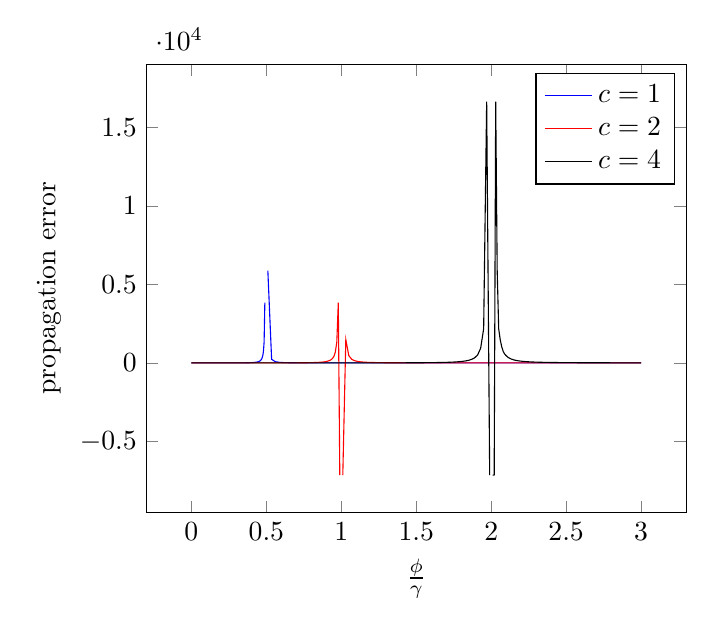
\begin{tikzpicture}
        \begin{axis}[ 
            xlabel=$\frac{\phi}{\gamma}$,
            ylabel={\pe}
        ] 
        \addplot [samples=100, domain=0:0.49, color=blue]{1/(1-e^((-1/(x)*(1-2*x)^2)/(2)))}; 
        \addplot [forget plot, samples=100, domain=0.51:3, color=blue]{1/(1-e^((-1/(x)*(1-2*x)^2)/(2)))}; 
        \addplot [samples=100, domain=0:0.99, color=red]{1/(1-e^((-1/(1/2*x)*(1-x)^2)/(2)))}; 
        \addplot [forget plot,samples=100, domain=1.01:3, color=red]{1/(1-e^((-1/(1/2*x)*(1-x)^2)/(2)))};
        \addplot [samples=100, domain=0:1.99, color=black]{1/(1-e^((-1/(1/4*x)*(1-1/2*x)^2)/(2)))}; 
        \addplot [forget plot,samples=100, domain=2.01:3, color=black]{1/(1-e^((-1/(1/4*x)*(1-1/2*x)^2)/(2)))};
        \addlegendentry{$c=1$}
        \addlegendentry{$c=2$}
        \addlegendentry{$c=4$}
    \end{axis}
    \end{tikzpicture}
    \caption{The \pe\ as function of $\frac{\phi}{\gamma}$}
    \label{fig:prop_err}
\end{figure}
\end{maybeappendix}

In order to analyse the \eve\ we will have to reason about the probability of HH flows to evict each other from the \cs\ and about the probability of non HH flows to evict HH flows from the \cs.

It is trivial to see that the probability of a HH flow to evict another HH flow from the \cs\ is controlled by the size of the \cs, $M$. Since there are at most $\frac{1}{\phi}$ heavy hitter flows, the probability of being evict by another HH is at most $\frac{\frac{1}{\phi}-1}{M}$ and it is enough to choose $\frac{1}{\phi} << M$ to get this probability as small as we wish.

\ignore{
\begin{lemma}
\label{lemma:nonhhhevic1}
Given a HH flow in the \cs\ with estimation $v_i$, the probability of being evicted by a non HH flow is $o(1)$.
\end{lemma}
\begin{proof}
In order for a non HH to evict a HH, it should go through the following steps: (1) enter the \sfa, (2) get propagated to the \cs\ and (3) evict the HH flow. The probability of the first step is $\frac{1}{v_0}$, the probability of the second step is at most $\frac{1}{v_0}$ (since it could get evicted itself from the \sfa) and the probability of the last step is $\frac{v_0}{v_i}$. Thus, the probability of evicting the HH flow is at most $\frac{1}{v_0v_i}$ which can be small as we wish by controlling $v$ since $v_0=v\phi N$.
\end{proof}
}
\begin{theorem}
\label{lemma:nonhhhevict}
Given a \cs\ of size $M$, and a HH flow $f$ with estimation $v_i$, the probability of $f$ being evicted by a non HH flow $g$ is at most $1/(M v N \phi \gamma_g^2 v_i)$.
\end{theorem}
\begin{proof}
In order for a non HH flow to evict a HH flow, it should go through the following steps: (1) enter the \sfa, (2) get propagated to the \cs\, (3) collide with $f$ when being hashed with $h_2$, and (4) evict $f$. The probability of the first step is at most $\frac{1}{v_0 \gamma_g}$, the probability of the second step is at most $\frac{1}{v_0 \gamma_g}$ (since it could get evicted itself from the \sfa), the probability of the third step is $\frac{1}{M}$ and the probability of the last step is $\frac{v_0}{v_i}$. Thus, the probability of evicting the HH flow $f$ by non HH flow $g$ is at most $\frac{1}{M v N \phi \gamma_g^2 v_i}$ which approaches $0$ as $M$ grows and can be small as we wish by controlling $v$.
\end{proof}

From the observation about the small as we wish probability of HH flows evicting each other and from Theorem~\ref{lemma:nonhhhevict}, we conclude that \eve\ is constant. Later our evaluation shows that after certain size of the \cs, there is no more effect on the algorithm's Detection Rate and False Positive Rate, supporting the claim that by increasing $M$ one can lower the \eve.

\begin{maybeappendix}{theory}

propagate to the \cs. Lemma~\ref{lemma:prop} reasons about the probability of propagating a given flow to the \cs\ given its size.

\begin{lemma}
\label{lemma:prop}
Given a flow $f$ of frequency $\gamma N$ ($0\leq \gamma \leq 1)$, then the probability of propagating to the \cs\  from the \sfa\ of size $\frac{c}{\phi}$, is at most $e^{\frac{-\frac{1}{m}(1-2m)^2}{3-2m}}$, where $m=\frac{\phi}{\gamma c}$.
\end{lemma}
\begin{proof}
Follows from Lemma~\ref{lemma:upper_tail} with $\frac{(1+\delta)|B|k}{|A|}=2$, since a flow will propagate to the \cs\ if and only if there are at least 2 occurrences in $\frac{c}{\phi}$ packets which is the size of \sfa.
\end{proof}

Lemma~\ref{lemma:avg_prop} conjectures on the probability of propagating the average non heavy hitter flow. Let us assume $F$ active flows in the trace where $H$ of them are true heavy hitters (we note that $H\leq\frac{1}{\phi})$, and that the portion of the true heavy hitters flows is $\phi_H$. Since usually that are much more active flows that heavy hitter flows ($H<<F$) \ignore{and the portion of heavy hitter flow is much bigger than those of non heavy hitters flows ($(1-\phi_H) << 1$)}, it makes sense to assume uniformity in the distribution of sizes of the non heavy hitter flows. Thus, the average frequency of a non heavy hitter flow is $\Bar{\gamma} = \frac{1-\phi_H}{F-H}$.

\begin{lemma}
\label{lemma:avg_prop}
The probability of propagating a non heavy hitter flow from a trace with $F$ active flows and $H$ heavy hitter flows of total portion $\phi_H$, is at most
$e^{\frac{-\frac{1}{\bar{m}}(1-2\bar{m})^2}{3-2\bar{m}}}$ where $\bar{m}=\frac{\phi}{c\bar{\gamma}}$.
\end{lemma}
\begin{proof}
Follows from Lemma~\ref{lemma:prop} and the above explanation.
\end{proof}

In Lemma~\ref{lemma:eve} we propose an upper bound on the probability of evicting a true heavy hitter flow from the \cs. While this probability is not bounded, it can be reduced by increasing $M$ and we will show later in the evaluation section that eviction does not happen of any practical settings. 

\begin{lemma}
\label{lemma:eve}
Given a \cs\ of size $M$ and a true heavy hitter flow $f$ and let us denote by $p$ the probability of an average non heavy hitter flow to propagate to the \cs\ presented in Lemma~\ref{lemma:avg_prop}, then the probability of $f$ to be evicted from the candidate set is at most $p^{M-(\frac{1}{\phi}-1)}$.
\end{lemma}
\begin{proof}
A true heavy hitter flow will be evicted from \cs\ if and only if the \cs\ becomes full. Since $M > \frac{1}{\phi} \geq H$, it will be evicted if enough non heavy hitter flows will be propagated, i.e. if $M-(H-1)$ non heavy hitter flows was propagated. This will happen with probability $p^{M-(H-1)}$.
\end{proof}

\ignore{
\begin{figure}
    \centering
    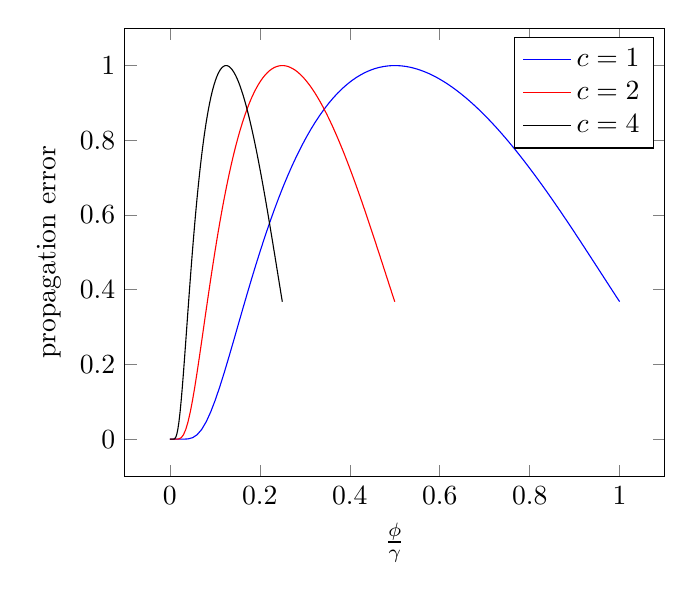
\begin{tikzpicture}
        \begin{axis}[ 
            xlabel=$\frac{\phi}{\gamma}$,
            ylabel={\pe}
        ] 
        \addplot [samples=100, domain=0:1, color=blue]{e^((-1/(x)*(1-2*x)^2)/(3-2*x))}; 
        \addplot [samples=100, domain=0:0.5, color=red]{e^((-1/(2*x)*(1-4*x)^2)/(3-4*x))}; 
        \addplot [samples=100, domain=0:0.25, color=black]{e^((-1/(4*x)*(1-8*x)^2)/(3-8*x))}; 
        \addlegendentry{$c=1$};
        \addlegendentry{$c=2$};
        \addlegendentry{$c=4$};
    \end{axis}
    \end{tikzpicture}
    \caption{The \pe\ as function of $\frac{\phi}{\gamma}$}
    \label{fig:eve}
\end{figure}
}
\end{maybeappendix}
\section{Analysis of Errors}
\label{sec:theory}
In this section we study the types of errors introduced by our algorithm and provide an analysis for each of them. In order to do so we denote by $F_{h_1(f)}$ the set of flows that are mapped to the same entry by $h_1$ as $f$, i.e., $F_{h_1(f)} = \{g\in F | h_1(g)=h_1(f)\}$, and by $\gamma_f$ the portion of flow $f$ from the whole trace, i.e., $\gamma_f N$ is the number of packets of flow $f$. Furthermore, we denote by $\Gamma_f$ the sum of portions of flows mapped to the same entry as $f$ by $h_1$, i.e., $\Gamma_f=\sum_{g\in F_{h_1(f)}} \gamma_g$.

The total error in the frequency estimation of a HH flow might originate from the various parts of the algorithm. The first type of error type is the \textit{\ee} which originates from the usage of shared estimators in the \sea. This relative error is bounded by $\delta$ as guaranteed from the original CEDAR scheme.

The second error type, which we denote by \textit{\pe}, is the error introduced to the estimation of HH flows for not propagating early enough from the \sfa\ to the \cs. While indeed, the algorithm will give a frequency estimation within the relative error of the true frequency for any flow in the \cs, however, this estimation holds from the moment the flow was propagated to the \cs, and this propagation does not happen on the first packet of the flow. The \pe\ captures the number of times the flow appeared in the trace before propagating to \cs.

When examining the $i^{th}$ and the ${i+1}^{th}$ packets of a HH flow $f$ (for $i\geq 2$), the probability of $f$ being evicted from the \sfa\ before propagating to the \cs\ is $\frac{\Gamma_f-\gamma_f}{\Gamma_f}$. This is true, since $\Gamma_F-\gamma_f$ is the portion of the flows but $f$ that are mapped to the same entry as $f$. Furthermore, the probability of a HH flow $f$ not to propagate to the \cs\ after $i+1$ packets is $\left(\frac{\Gamma_f-\gamma_f}{\gamma_g}\right)^{i}$, which approaches $0$ as more packets for flow $f$ arrive.

The last type of error, which we denote by \textit{\eve}, is the error introduced to the estimation of HH flows due to the eviction of such flows from the \cs. These evictions happen when there is a collision in $h_2$, then the algorithm evicts the currently tracked flow with a low probability of $\frac{v_0}{v_i}$. The motivation of evicting with this probability is to replace the current flow, only if the new flow had arrived many times. However, evictions of HH flows could still occur due to the possible collisions in $h_2$ with other HH flows.

Since $h_2$ is a uniform hash function, the expected number of collisions between HH flows is given by $\frac{h(h-1)}{2M}$ where $h$ is the number of HH flows and $M$ is the number of entries in the \cs. It is clear that the more memory used for the \cs\ the less expected collisions we will have in $h_2$ and the smaller the \eve.

\begin{figure*}
\begin{subfigure}[t]{0.32\textwidth}
    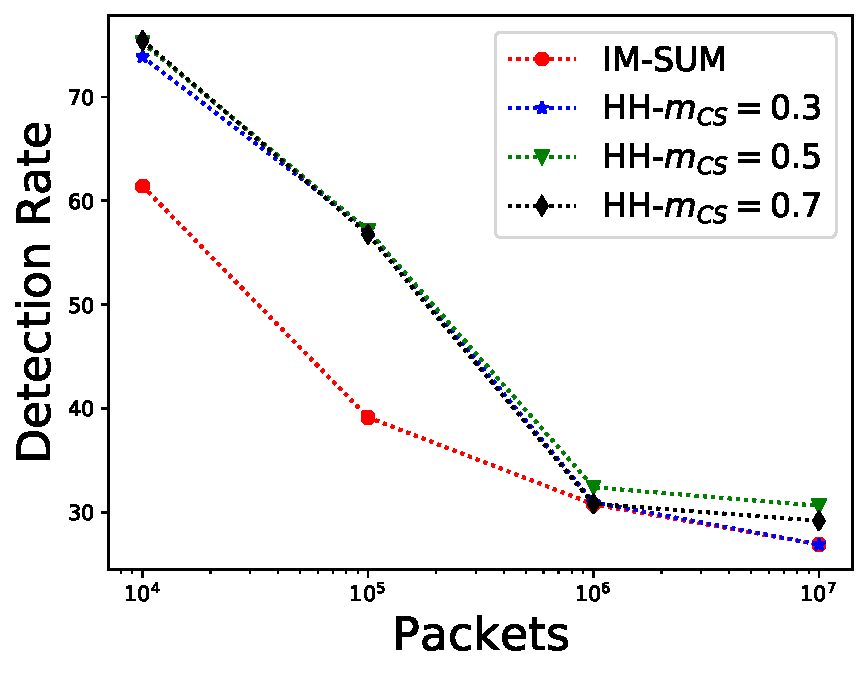
\includegraphics[width=\linewidth]{HH/figures/DR_per_pkts_m=0.03125.pdf}
    \caption{32KB}
    \label{fig:fig2_a}    
\end{subfigure}\hfill
\begin{subfigure}[t]{0.32\textwidth}
    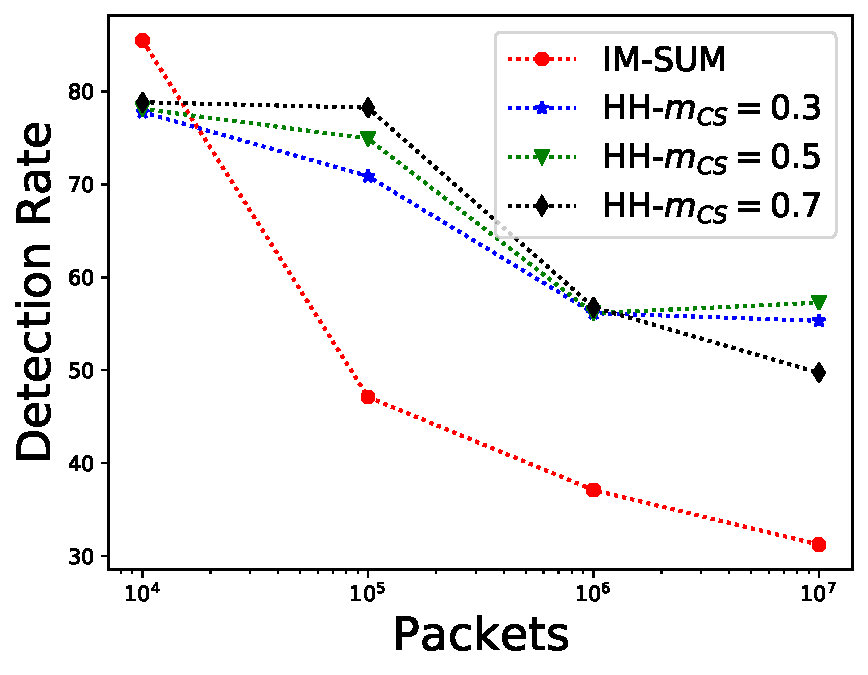
\includegraphics[width=\linewidth]{HH/figures/DR_per_pkts_m=0.0625.pdf}
    \caption{64KB}
    \label{fig:fig2_b}
\end{subfigure}\hfill
\begin{subfigure}[t]{0.32\textwidth}
    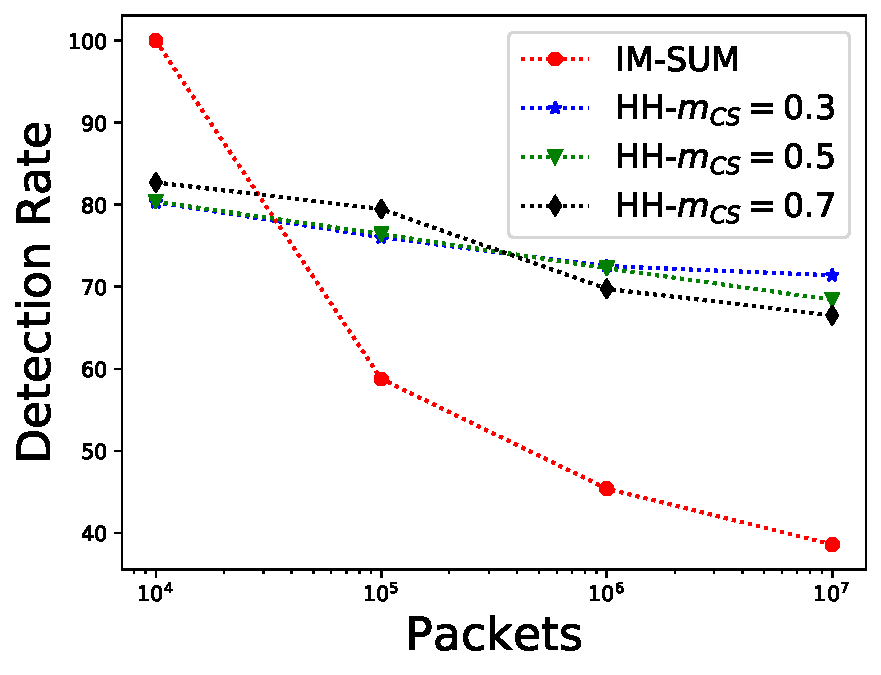
\includegraphics[width=\linewidth]{HH/figures/DR_per_pkts_m=0.125.pdf}
    \caption{128KB}
    \label{fig:fig2_c}
\end{subfigure}

\begin{subfigure}[t]{0.32\textwidth}
    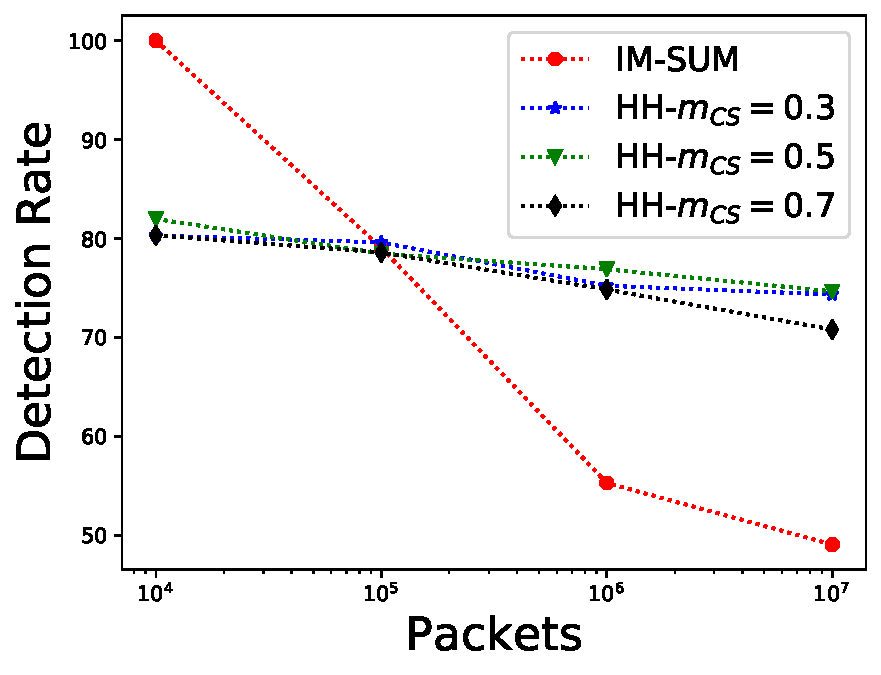
\includegraphics[width=\linewidth]{HH/figures/DR_per_pkts_m=0.25.pdf}
    \caption{0.25MB}
    \label{fig:fig2_d}
\end{subfigure}\hfill
\begin{subfigure}[t]{0.32\textwidth}
    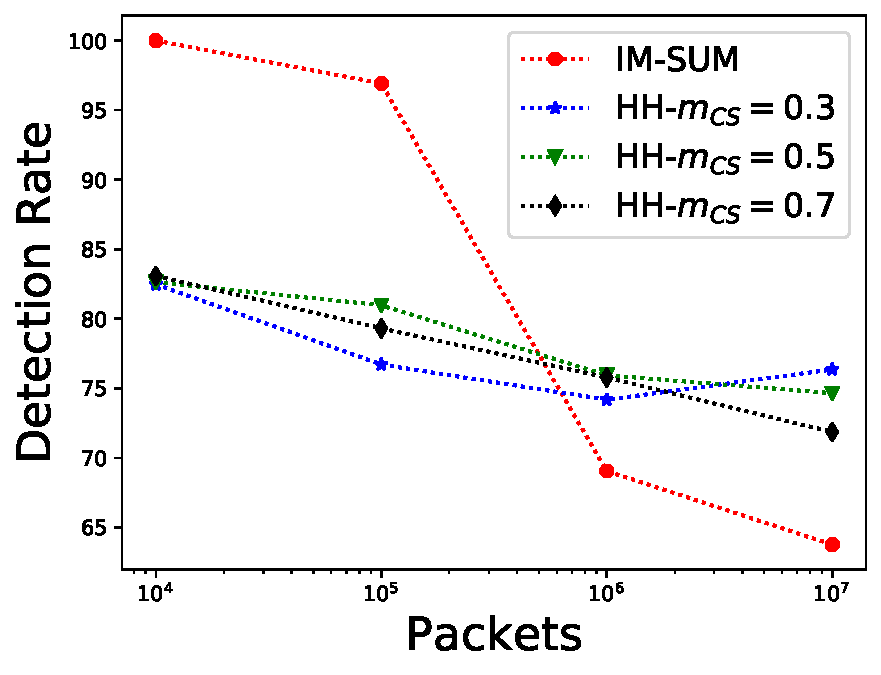
\includegraphics[width=\linewidth]{HH/figures/DR_per_pkts_m=0.5.pdf}
    \caption{0.5MB}
    \label{fig:fig2_e}
\end{subfigure}\hfill
\begin{subfigure}[t]{0.32\textwidth}
    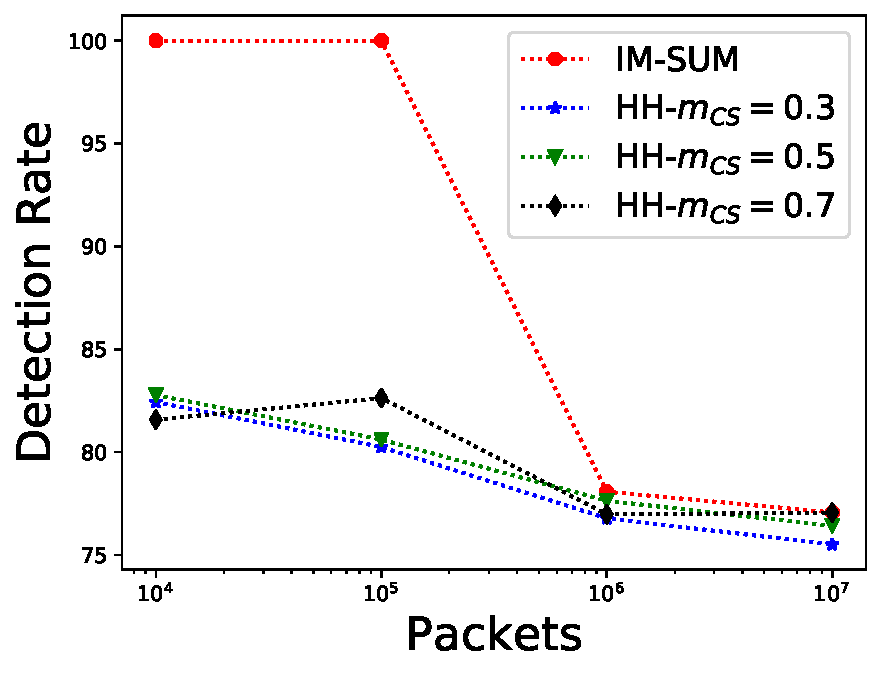
\includegraphics[width=\linewidth]{HH/figures/DR_per_pkts_m=1.0.pdf}
    \caption{1MB}
    \label{fig:fig2_f}
\end{subfigure}

\caption{The Average Detection Rate as function of number of packets, comparing our algorithm in three different settings vs. the Elephants algorithm for $\phi=0.001,\delta=0.05$}
\label{figure2}
\end{figure*}

\begin{figure*}
\begin{subfigure}[t]{0.32\textwidth}
    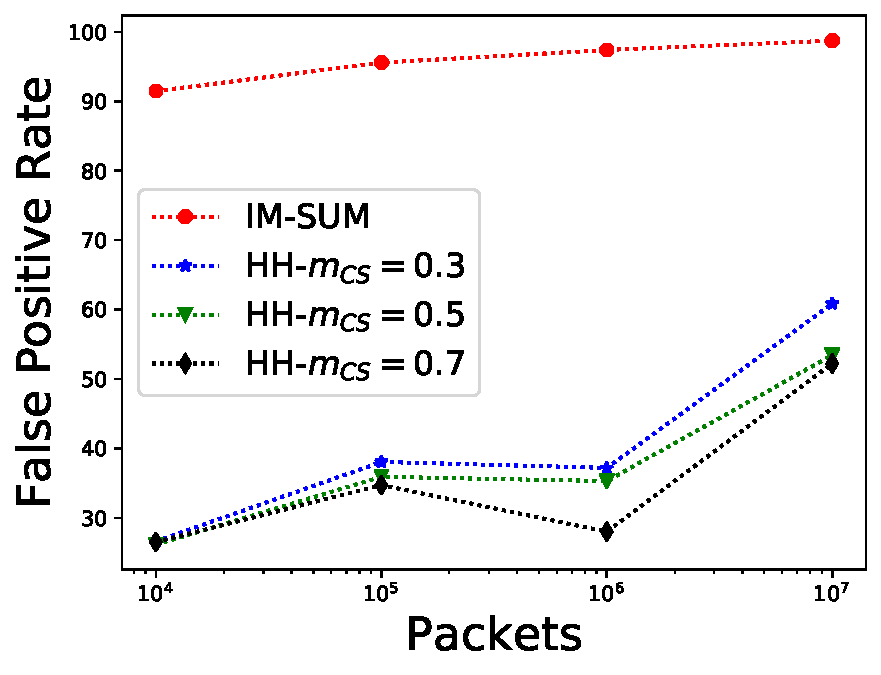
\includegraphics[width=\linewidth]{HH/figures/FPR_per_pkts_m=0.03125.pdf}
    \caption{32KB}
    \label{fig:fig3_a}    
\end{subfigure}\hfill
\begin{subfigure}[t]{0.32\textwidth}
    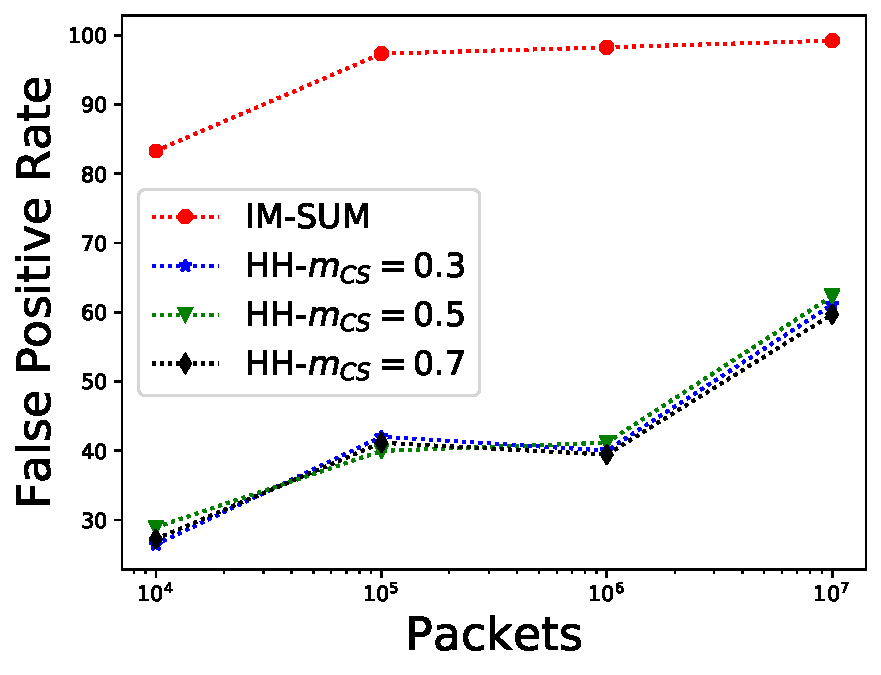
\includegraphics[width=\linewidth]{HH/figures/FPR_per_pkts_m=0.0625.pdf}
    \caption{64KB}
    \label{fig:fig3_b}
\end{subfigure}\hfill
\begin{subfigure}[t]{0.32\textwidth}
    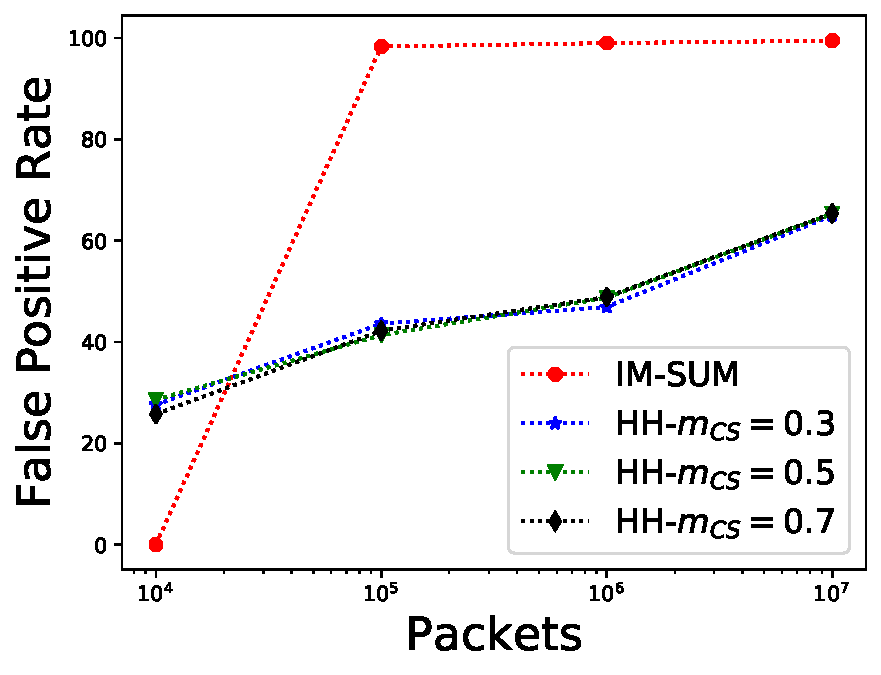
\includegraphics[width=\linewidth]{HH/figures/FPR_per_pkts_m=0.125.pdf}
    \caption{128KB}
    \label{fig:fig3_c}
\end{subfigure}

\begin{subfigure}[t]{0.32\textwidth}
    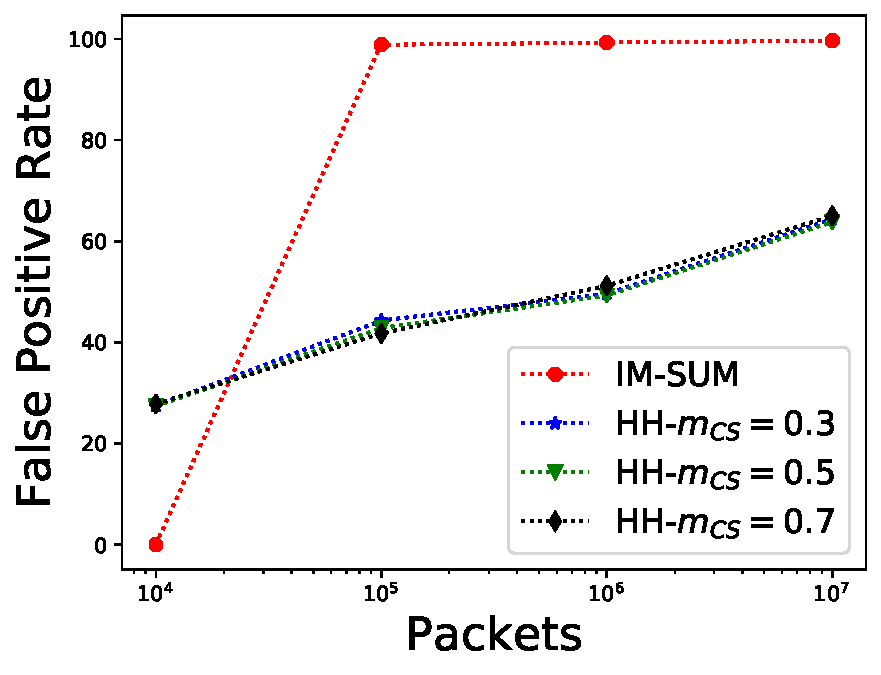
\includegraphics[width=\linewidth]{HH/figures/FPR_per_pkts_m=0.25.pdf}
    \caption{0.25MB}
    \label{fig:fig3_d}
\end{subfigure}\hfill
\begin{subfigure}[t]{0.32\textwidth}
    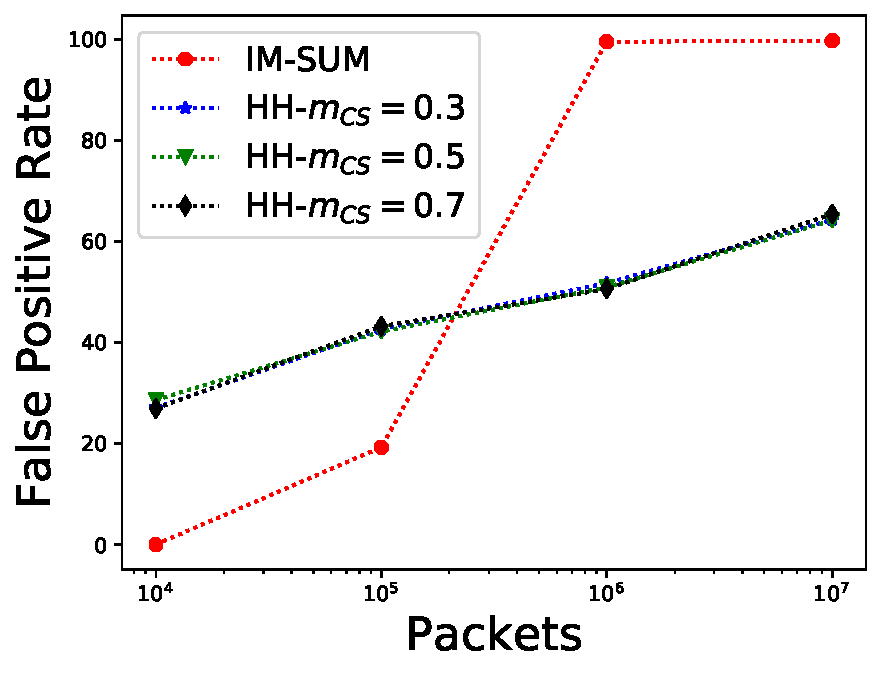
\includegraphics[width=\linewidth]{HH/figures/FPR_per_pkts_m=0.5.pdf}
    \caption{0.5MB}
    \label{fig:fig3_e}
\end{subfigure}\hfill
\begin{subfigure}[t]{0.32\textwidth}
    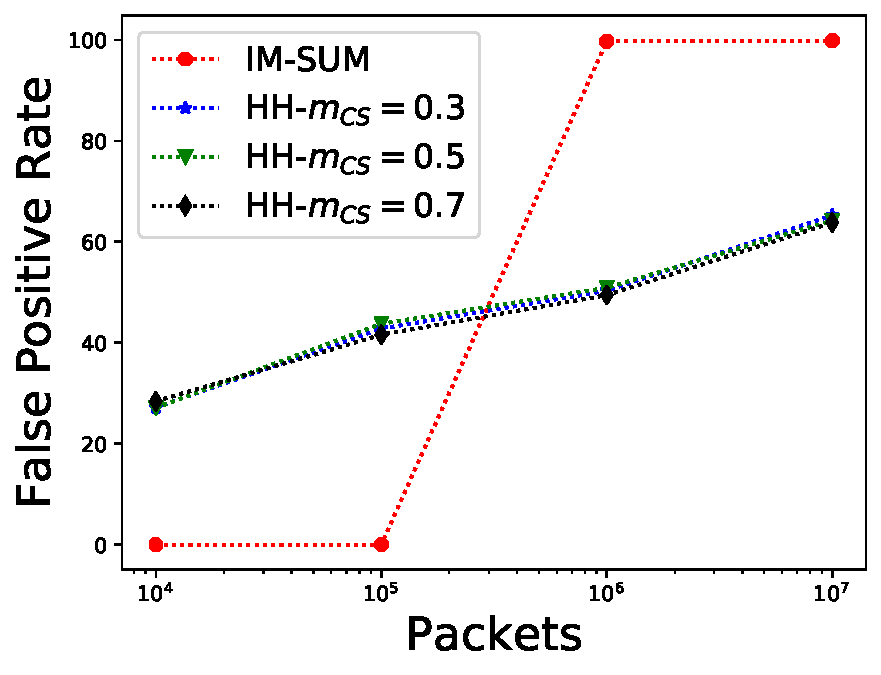
\includegraphics[width=\linewidth]{HH/figures/FPR_per_pkts_m=1.0.pdf}
    \caption{1MB}
    \label{fig:fig3_f}
\end{subfigure}

\caption{The Average False Positive Rate as function of number of packets, comparing our algorithm in three different settings vs. the Elephants algorithm for $\phi=0.001,\delta=0.05$}
\label{figure3}
\end{figure*}
\section{Evaluation}
\label{sec:evaluation}
\subsection{Settings}
In order to evaluate the performance of our algorithms, we implemented them and a version of the IM-SUM algorithm from~\cite{basat2017optimal}. We evaluated the algorithms on the newest CAIDA Anonymized Internet Traces Dataset, the CAIDA`19 New-York dataset~\cite{CAIDA2019}.

For all of the evaluation, unless stated otherwise, we used the following: (1) IPv4 5-tuple flows with $|flow\_id|=104$, (2) HH threshold, $\phi=0.001$, (3) $\delta=0.05$, (4) each datapoint is the average of 10 runs, each starting in a random packet in the trace, (5) the \sea\ memory is 1\% of the available memory ($m_{SEA}=0.01)$ and (6) a propagation parameter, $v=0.35$.

To measure the performance of algorithms we used the following metrics:
\begin{itemize}
    \item Detection Rate (DR), the same as the previously mentioned Recall - which is the ratio of HH flows that the algorithm detected.
    \item False Positive Ratio (FPR) - which is the ratio of non HH flows reported by the algorithm as HH from the total number of reported flows.
    \item Throughput - the number of insertions the algorithm can perform per a single millisecond.
\end{itemize}

To be able to compare the algorithms we set the total memory available to use and the accuracy parameter. The memory usage of the IM-SUM algorithm is determined by the accuracy parameter, $\epsilon$, and its performance parameter, $\gamma$, which tunes the algorithm's memory-speed trade off.
In each run of IM-SUM, the amount of memory and the accuracy parameter was set, and we calculated the appropriate $\gamma$ for this run. For the \cs\ algorithm, the only tuning parameter is the partition of the left 99\% of the memory between the \cs\ and the \sfa\ ,i.e., setting $m_{CS}$ and $m_{SFA}=0.99-m_{CS}$.

The \cs\ algorithm and the IM-SUM algorithm provide different accuracy guarantees on the reported set of flows. The IM-SUM algorithm ensures accuracy in the range $[N(\phi-\epsilon),N \phi]$ while the \cs\ algorithm ensures accuracy in the range $[(1-\delta)\phi N, \phi N]$. The effective accuracy slack of the IM-SUM algorithm is $N\epsilon$, which is much larger than \cs's slack of $N\delta\phi$. Thus when comparing the algorithms with the same accuracy parameter, $\epsilon=\delta$, we give an edge to the IM-SUM algorithm, allowing it to possibly report more flows as HH than the \cs\ algorithm.

\subsection{Results}

\begin{figure*}
\begin{subfigure}[t]{0.32\textwidth}
    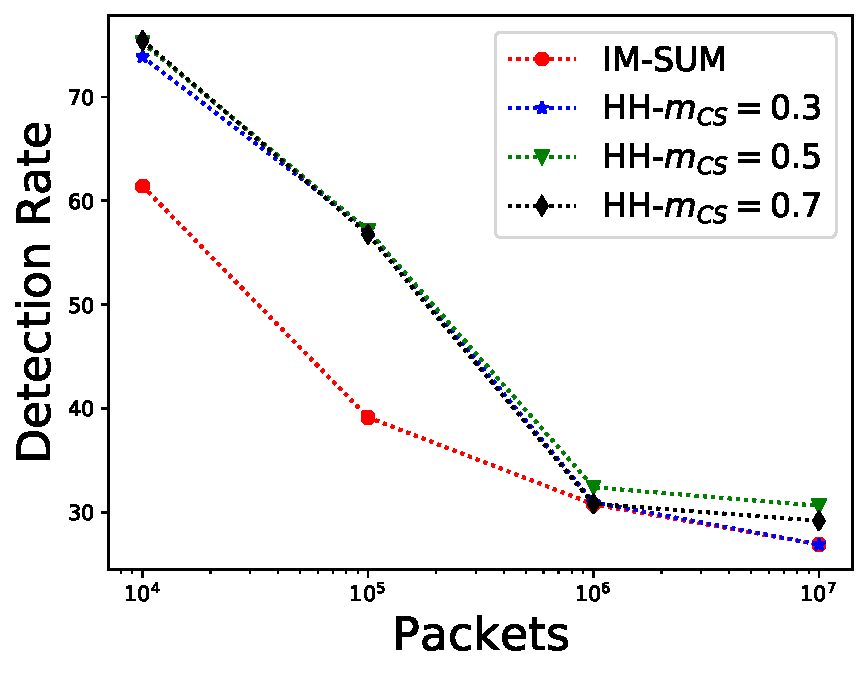
\includegraphics[width=\linewidth]{HH/figures/DR_per_pkts_m=0.03125.pdf}
    \caption{32KB}
    \label{fig:fig2_a}    
\end{subfigure}\hfill
\begin{subfigure}[t]{0.32\textwidth}
    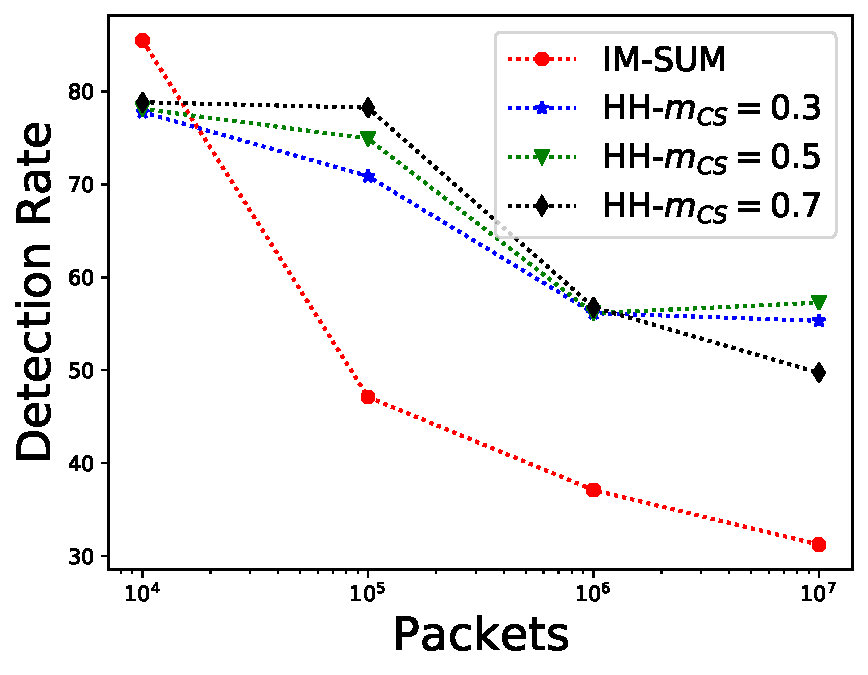
\includegraphics[width=\linewidth]{HH/figures/DR_per_pkts_m=0.0625.pdf}
    \caption{64KB}
    \label{fig:fig2_b}
\end{subfigure}\hfill
\begin{subfigure}[t]{0.32\textwidth}
    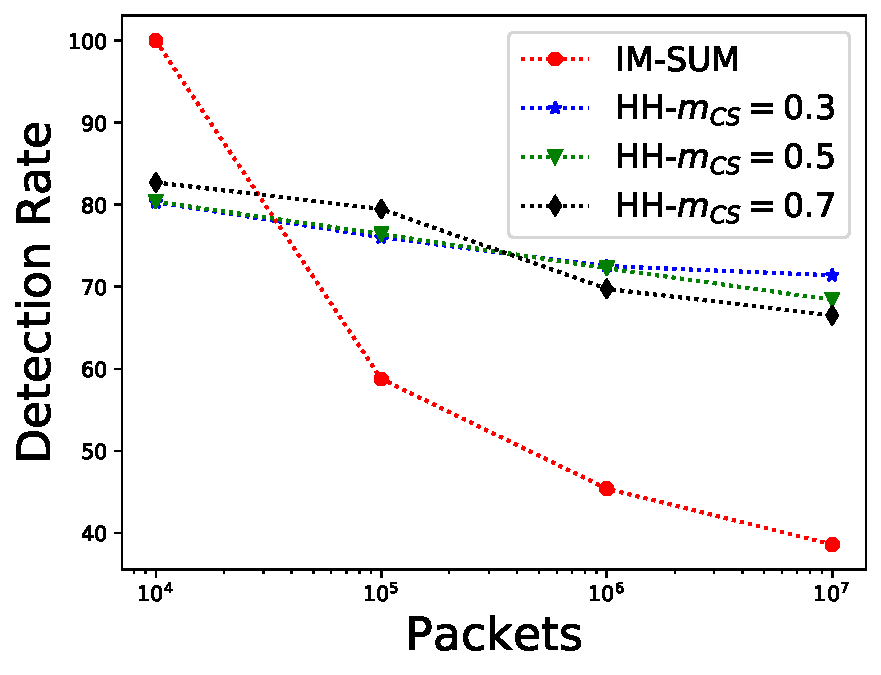
\includegraphics[width=\linewidth]{HH/figures/DR_per_pkts_m=0.125.pdf}
    \caption{128KB}
    \label{fig:fig2_c}
\end{subfigure}

\begin{subfigure}[t]{0.32\textwidth}
    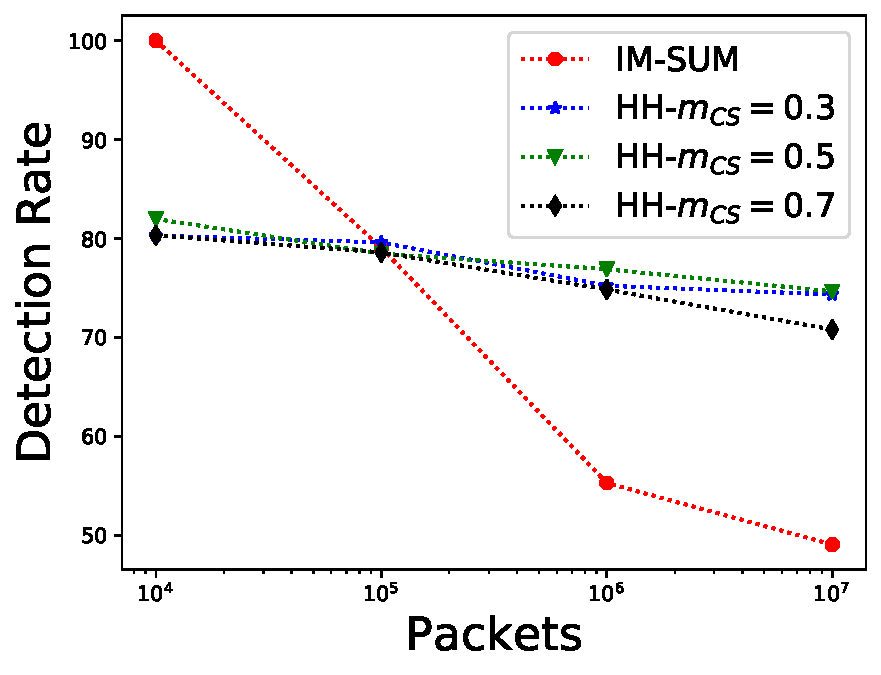
\includegraphics[width=\linewidth]{HH/figures/DR_per_pkts_m=0.25.pdf}
    \caption{0.25MB}
    \label{fig:fig2_d}
\end{subfigure}\hfill
\begin{subfigure}[t]{0.32\textwidth}
    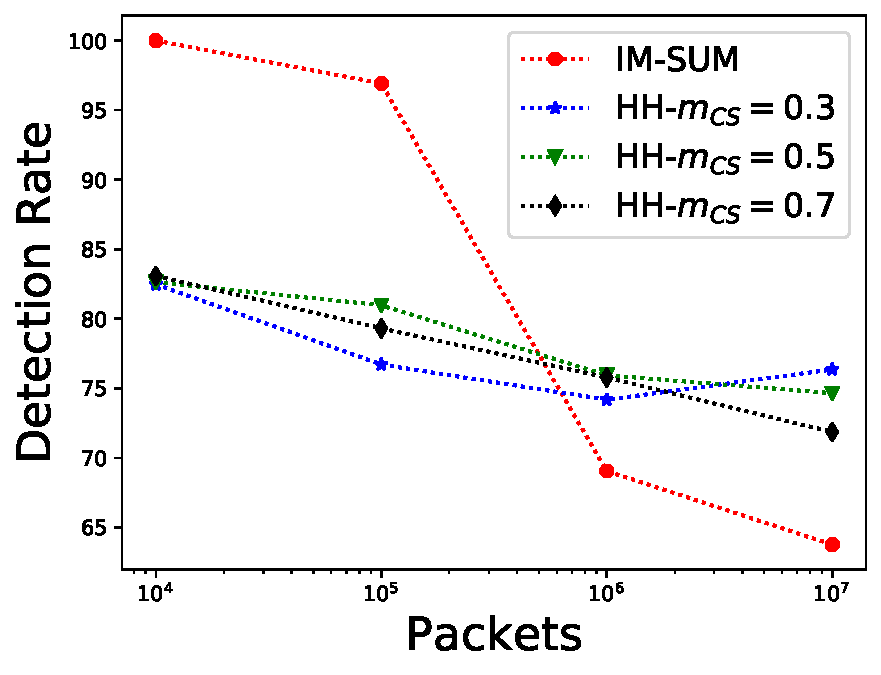
\includegraphics[width=\linewidth]{HH/figures/DR_per_pkts_m=0.5.pdf}
    \caption{0.5MB}
    \label{fig:fig2_e}
\end{subfigure}\hfill
\begin{subfigure}[t]{0.32\textwidth}
    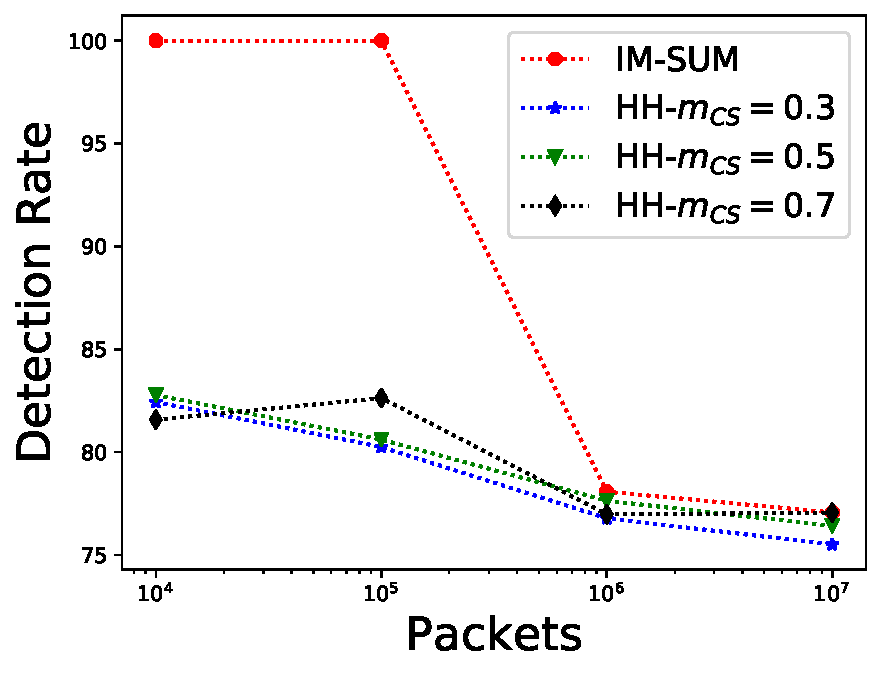
\includegraphics[width=\linewidth]{HH/figures/DR_per_pkts_m=1.0.pdf}
    \caption{1MB}
    \label{fig:fig2_f}
\end{subfigure}

\caption{The Average Detection Rate as function of number of packets, comparing our algorithm in three different settings vs. the Elephants algorithm for $\phi=0.001,\delta=0.05$}
\label{figure2}
\end{figure*}


Figures~\ref{fig:fig2_a}-~\ref{fig:fig2_f} show the average DR of the algorithms as a function of the number of packets processed. Intuitively, the DR relies heavily on the amount of available memory and one can see that the more memory allocated to the algorithms, the higher the DR rate is. When evaluating the \cs\ algorithm, we tested several variants with the different partition of the memory between the \cs\ and the \sfa. These variants allocates 30\%,50\%,70\% of the memory to the \cs\ and 69\%,49\%,29\% to the \sfa\ accordingly.

It is not clear how this trade off between the size of the \cs\ and the size of the \sfa\ affects the performance of the algorithm. When \cs\ is large the algorithm can hold on to ``big" flows while when  \sfa\ is large the algorithm can hold on to the more ``recent" flows. One can see that while the partition is balanced enough, that means there are no too few entries in the \sfa\ nor in the \cs\ and the effect on DR is small.

Figures~\ref{fig:fig2_a} and~\ref{fig:fig2_b} show that the \cs\ performs better than IM-SUM algorithm for amounts of memory smaller than 64KB and in some settings even finds 50\% more HH flows. However, it is worthy to note that, that both algorithm's DR degrades when processing more packets in this range of memories, which is unexpected since none of the algorithms guarantees relies on $N$.
Figures~\ref{fig:fig2_c} to~\ref{fig:fig2_f} show that this phenomenon of DR degradation when the number of packets increase is not present in the \cs\ algorithm compared to the IM-SUM algorithm.

However, this is not the case for the IM-SUM algorithm. The more memory the algorithm has the higher the DR, while the more packets processed the lower the DR. That is, for a given amount of memory our algorithm can process more packets without compromising its DR.

\begin{figure*}
\begin{subfigure}[t]{0.32\textwidth}
    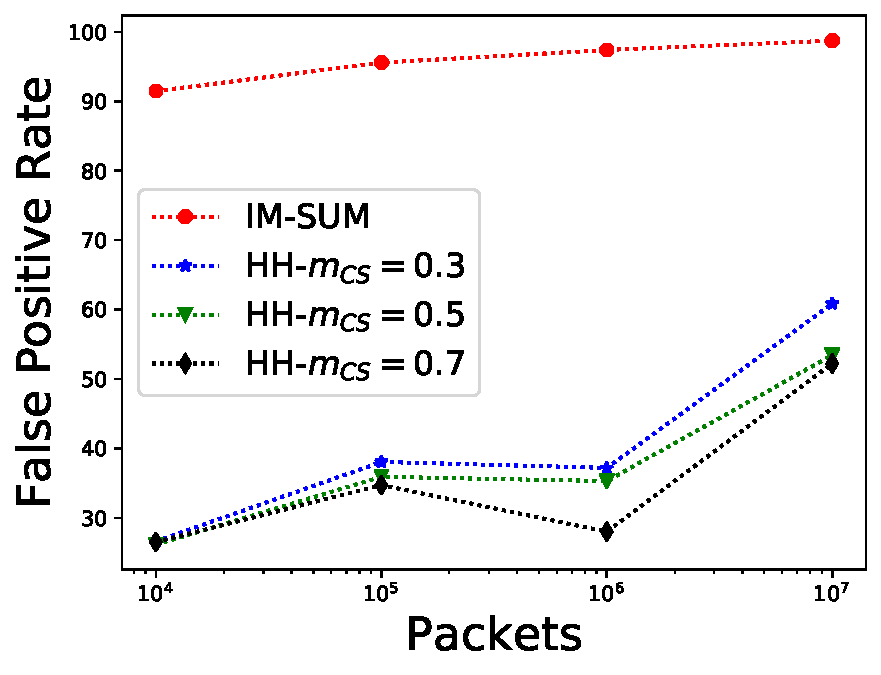
\includegraphics[width=\linewidth]{HH/figures/FPR_per_pkts_m=0.03125.pdf}
    \caption{32KB}
    \label{fig:fig3_a}    
\end{subfigure}\hfill
\begin{subfigure}[t]{0.32\textwidth}
    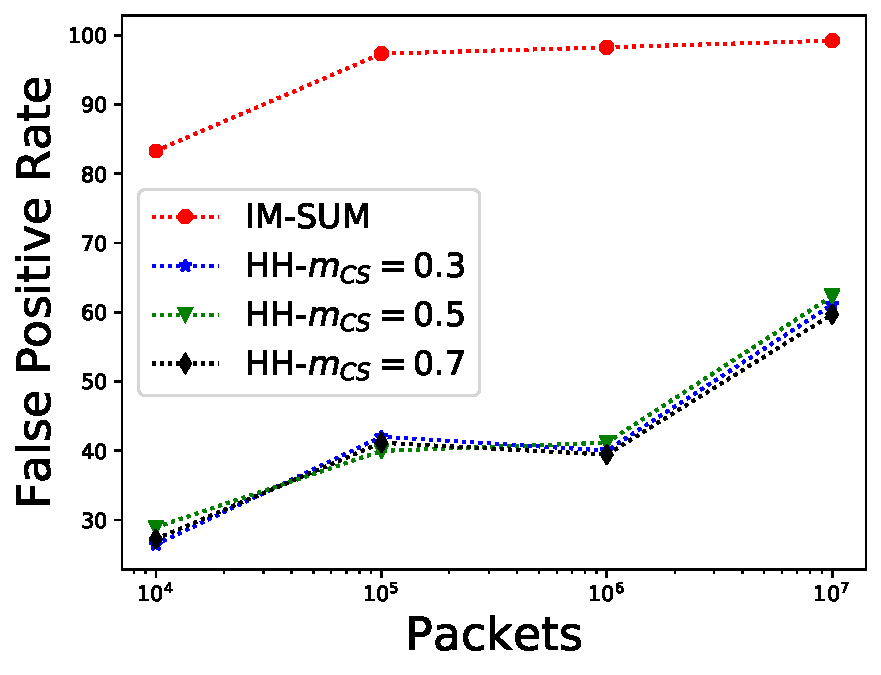
\includegraphics[width=\linewidth]{HH/figures/FPR_per_pkts_m=0.0625.pdf}
    \caption{64KB}
    \label{fig:fig3_b}
\end{subfigure}\hfill
\begin{subfigure}[t]{0.32\textwidth}
    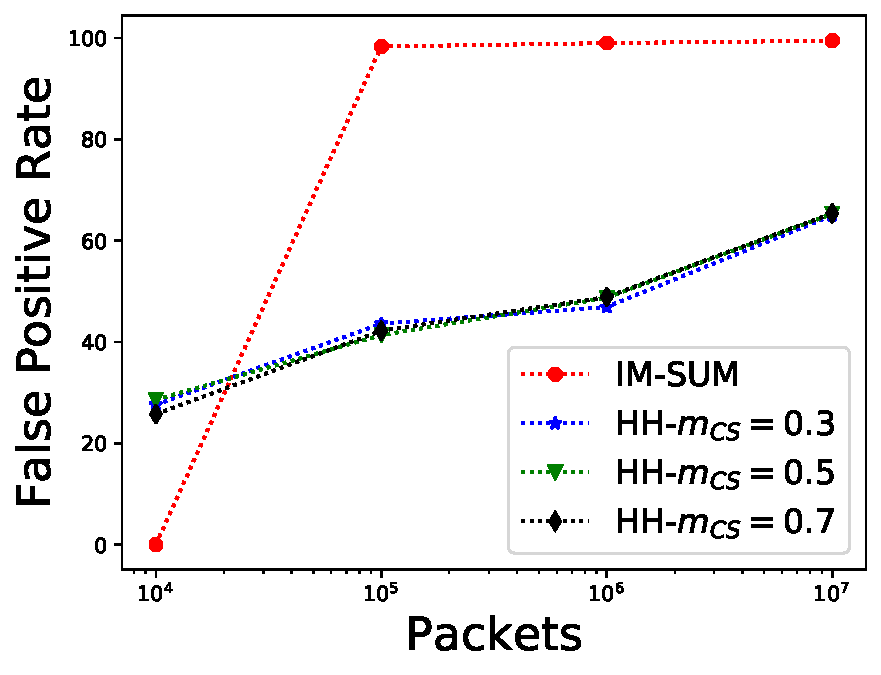
\includegraphics[width=\linewidth]{HH/figures/FPR_per_pkts_m=0.125.pdf}
    \caption{128KB}
    \label{fig:fig3_c}
\end{subfigure}

\begin{subfigure}[t]{0.32\textwidth}
    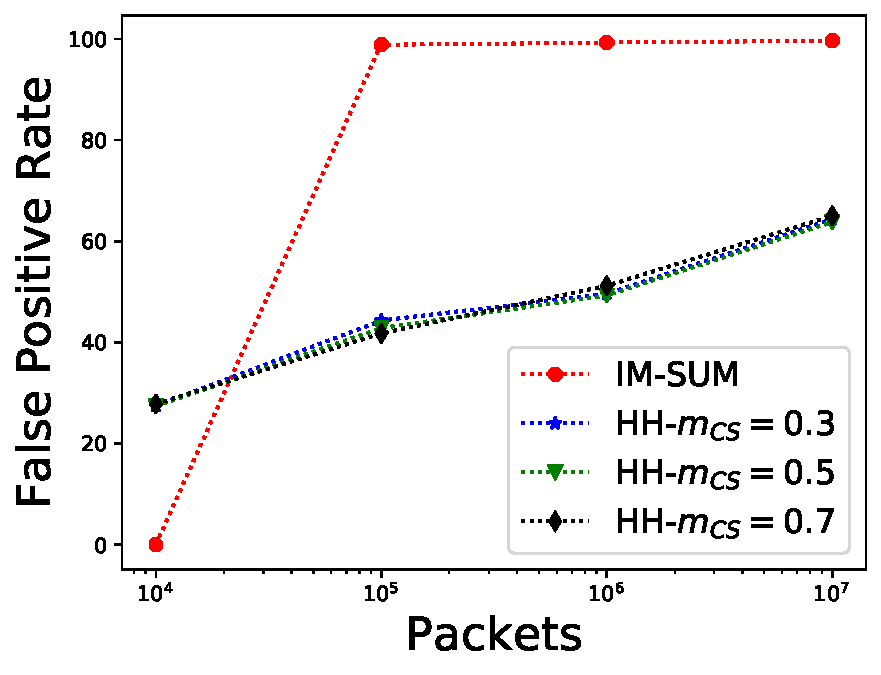
\includegraphics[width=\linewidth]{HH/figures/FPR_per_pkts_m=0.25.pdf}
    \caption{0.25MB}
    \label{fig:fig3_d}
\end{subfigure}\hfill
\begin{subfigure}[t]{0.32\textwidth}
    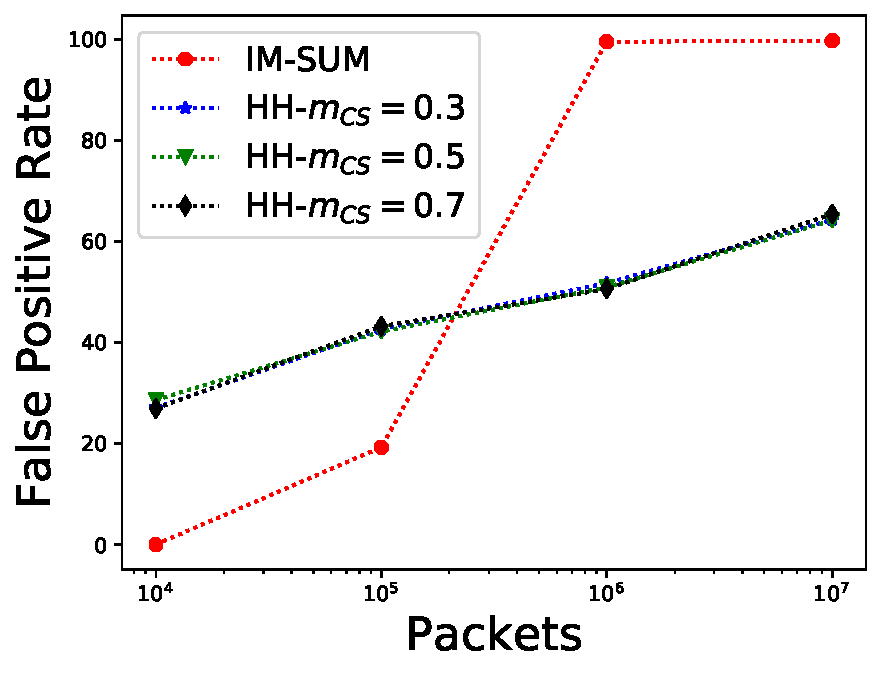
\includegraphics[width=\linewidth]{HH/figures/FPR_per_pkts_m=0.5.pdf}
    \caption{0.5MB}
    \label{fig:fig3_e}
\end{subfigure}\hfill
\begin{subfigure}[t]{0.32\textwidth}
    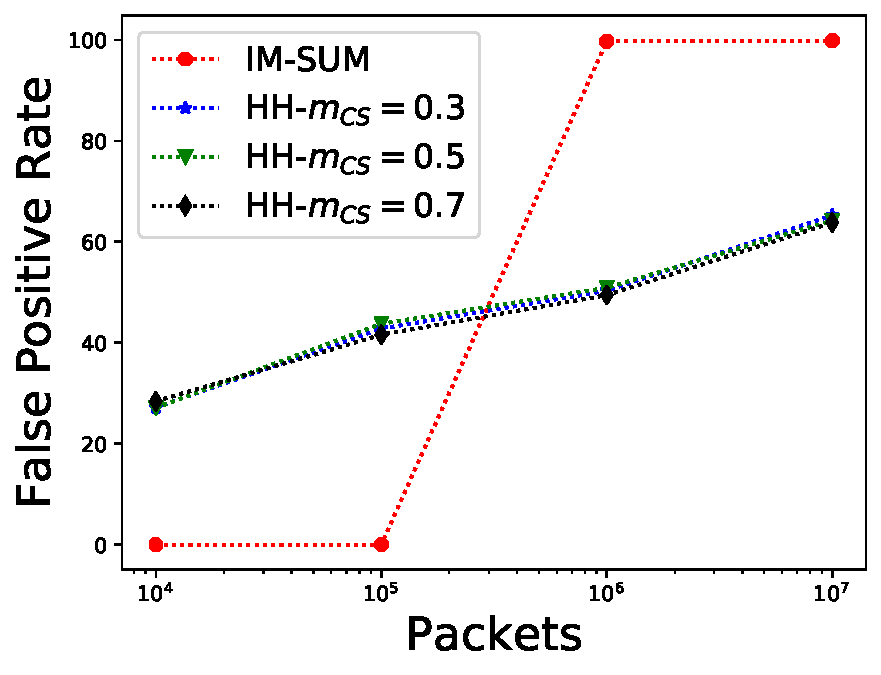
\includegraphics[width=\linewidth]{HH/figures/FPR_per_pkts_m=1.0.pdf}
    \caption{1MB}
    \label{fig:fig3_f}
\end{subfigure}

\caption{The Average False Positive Rate as function of number of packets, comparing our algorithm in three different settings vs. the Elephants algorithm for $\phi=0.001,\delta=0.05$}
\label{figure3}
\end{figure*}

Figures~\ref{fig:fig3_a}-~\ref{fig:fig3_f} show the average FPR of the algorithms as a function of the number of packets processed. It is worthy to note that the FPR of the \cs\ algorithm does not depend on the amount of memory, that is, using more memory does not affect the FPR. This is true since the algorithm's FPR depends directly on the estimation given by the \sea, and this estimation is always accurate up to $1\pm \delta$, regardless of the amount of memory. This also explains the lack of effect of the value of $m_{CS}$ on the FPR.

Interestingly, when the IM-SUM algorithm is given enough memory and not many packets, it will not report false positive flows. However, for each memory settings there is a number of packets where the algorithm starts reporting almost 100\% false positive flows, this means that the vast majority of the reported set of flows is non HH flows.

When considering the comparison of the algorithms in terms of FPR, it is evident that the \cs\ algorithm performs better. For less than $64KB$ it is always less than IM-SUM's FPR, while for larger amounts of memory it stays pretty constant in the range 40\%-60\% while IM-SUM's FPR soars quickly to around 100\%.

\begin{figure*}

\begin{subfigure}[t]{0.32\textwidth}
    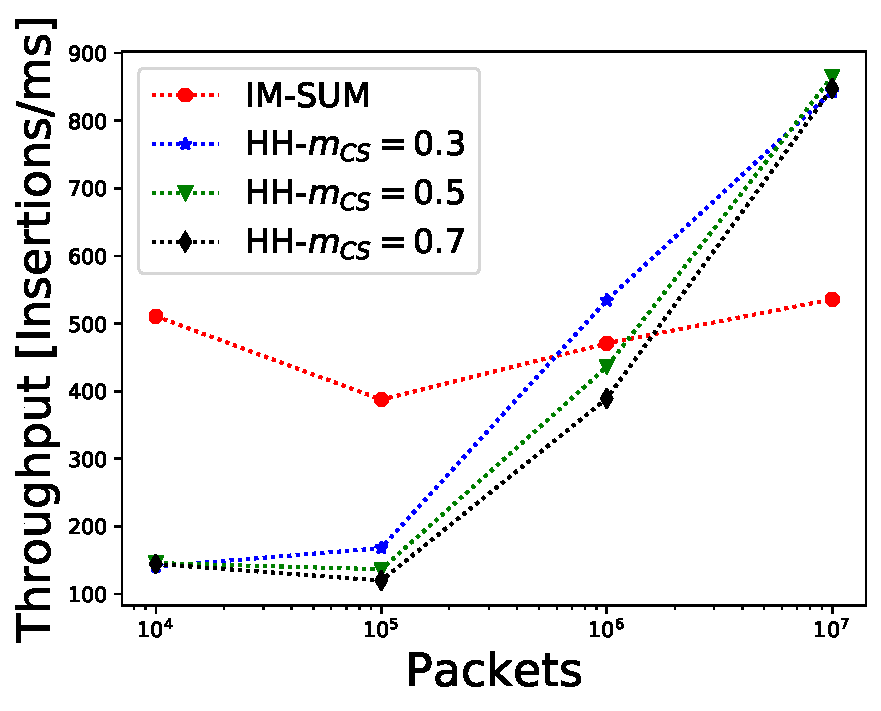
\includegraphics[width=\linewidth]{HH/figures/throughput_per_pkts_m=0.03125.pdf}
    \caption{32KB}
    \label{fig:fig4_a}    
\end{subfigure}\hfill
\begin{subfigure}[t]{0.32\textwidth}
    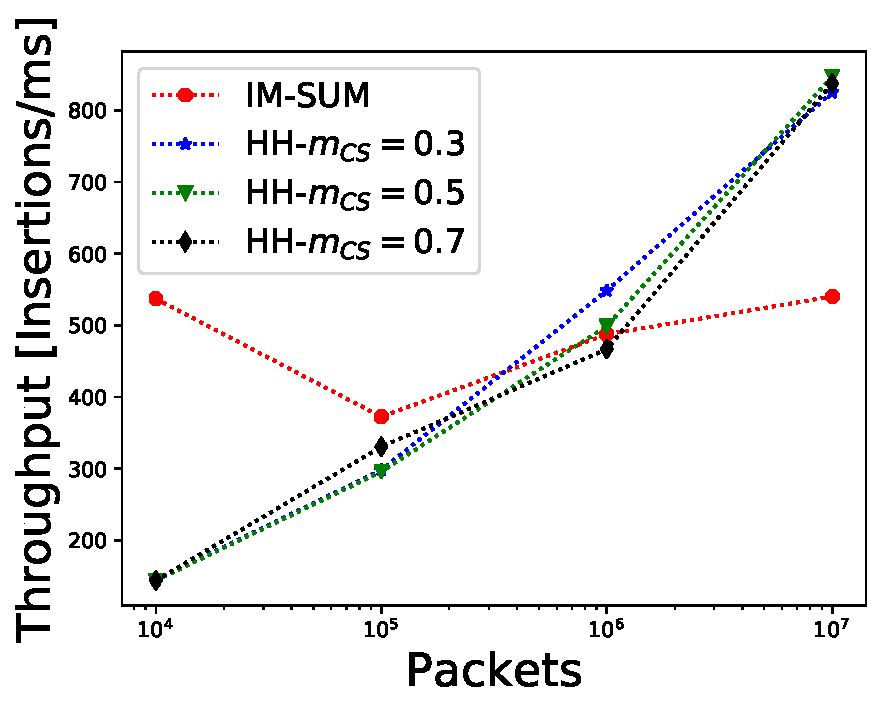
\includegraphics[width=\linewidth]{HH/figures/throughput_per_pkts_m=0.0625.pdf}
    \caption{64KB}
    \label{fig:fig4_b}
\end{subfigure}\hfill
\begin{subfigure}[t]{0.32\textwidth}
    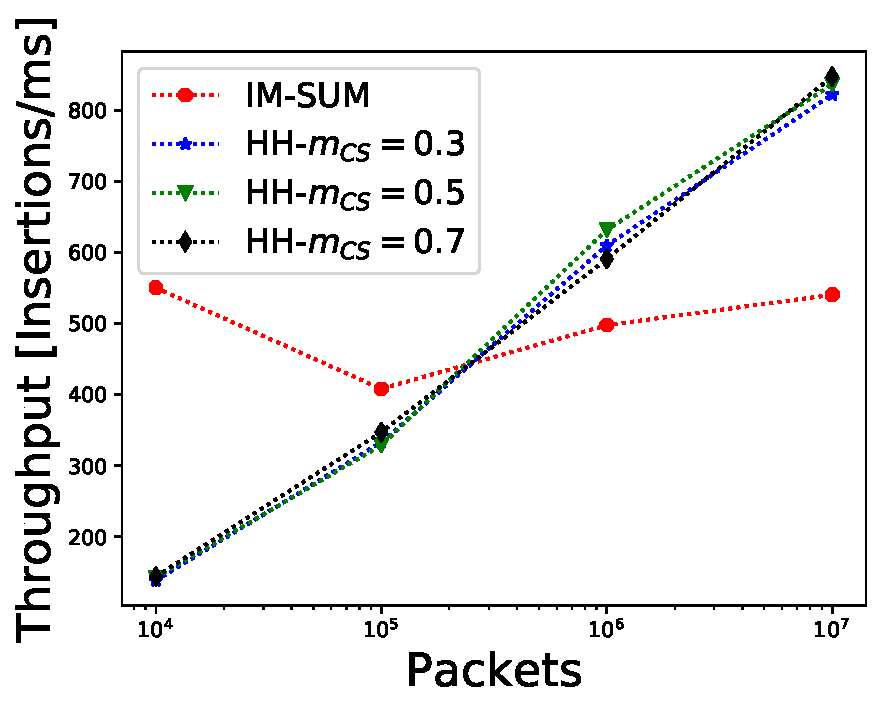
\includegraphics[width=\linewidth]{HH/figures/throughput_per_pkts_m=0.125.pdf}
    \caption{128KB}
    \label{fig:fig4_c}
\end{subfigure}

\begin{subfigure}[t]{0.32\textwidth}
    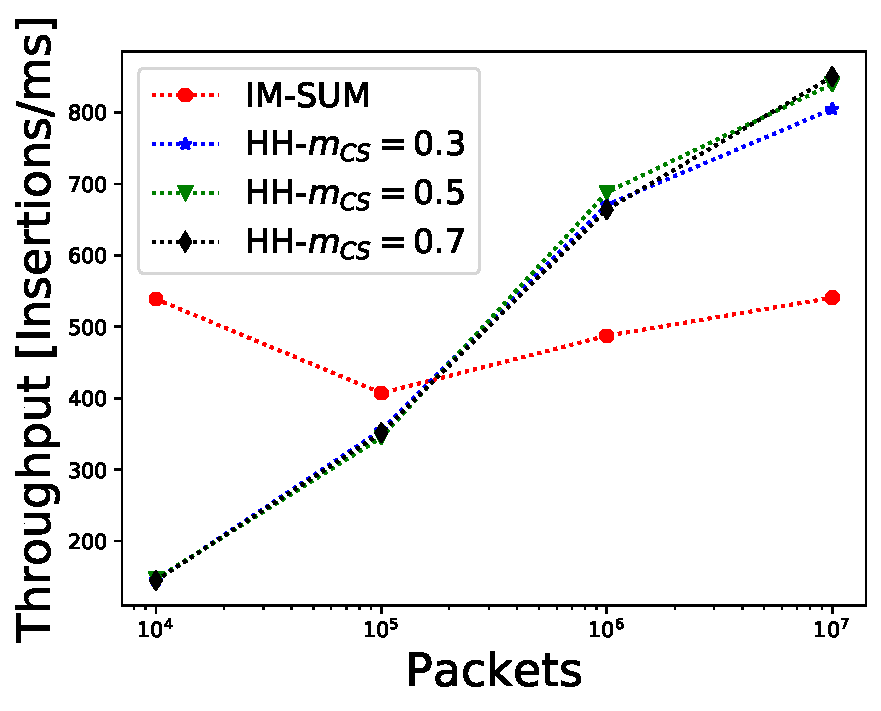
\includegraphics[width=\linewidth]{HH/figures/throughput_per_pkts_m=0.25.pdf}
    \caption{0.25MB}
    \label{fig:fig4_d}
\end{subfigure}\hfill
\begin{subfigure}[t]{0.32\textwidth}
    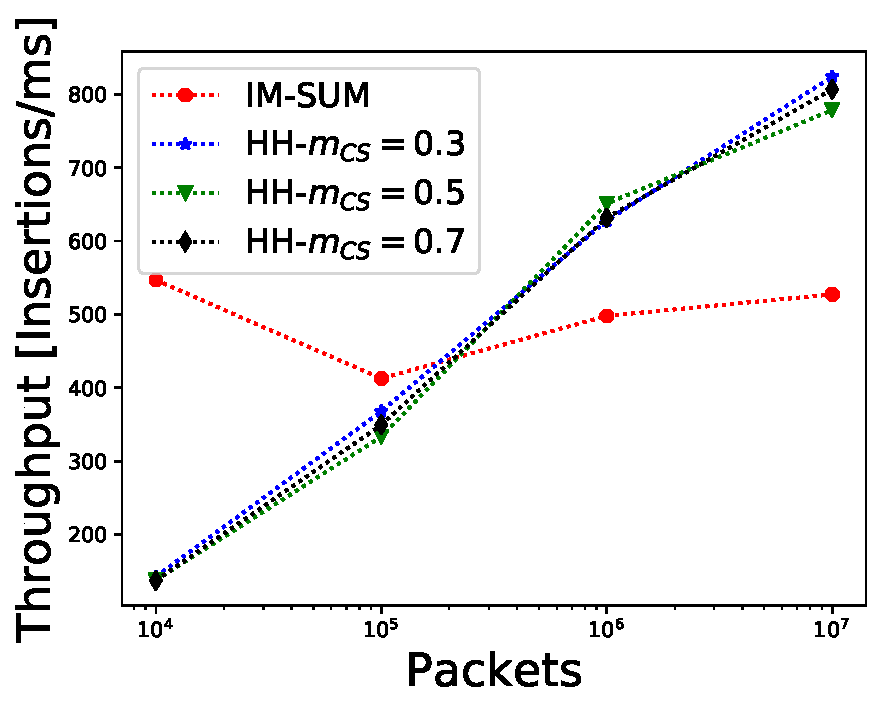
\includegraphics[width=\linewidth]{HH/figures/throughput_per_pkts_m=0.5.pdf}
    \caption{0.5MB}
    \label{fig:fig4_e}
\end{subfigure}\hfill
\begin{subfigure}[t]{0.32\textwidth}
    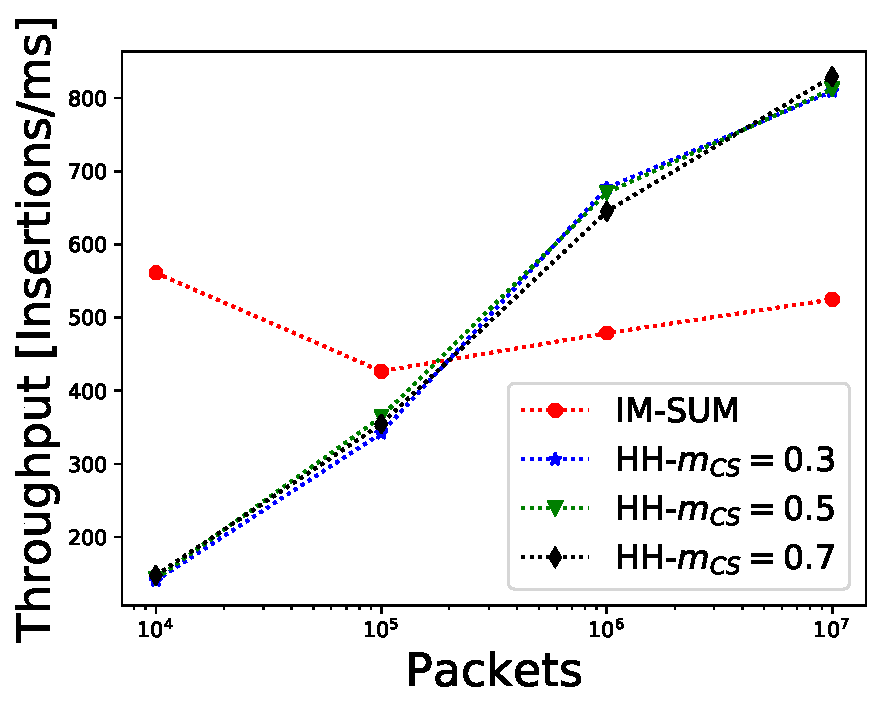
\includegraphics[width=\linewidth]{HH/figures/throughput_per_pkts_m=1.0.pdf}
    \caption{1MB}
    \label{fig:fig4_f}
\end{subfigure}

\caption{The Average Throughput as function of number of packets, comparing our algorithm in three different settings vs. the Elephants algorithm for $\phi=0.001,\delta=0.05$}
\label{figure4}
\end{figure*}

Figures~\ref{fig:fig4_a}-~\ref{fig:fig4_f} show the throughput in terms of insertions per millisecond of the algorithms as a function of the number of packets processed. For both algorithms, the more packets processed for a given amount of memory, the higher the throughput. In the case of IM-SUM, it seems that for $N=10^4$ we get the highest throughput. However, this datapoint is an anomaly since, with that few packets, the algorithm does not perform the heavy maintenance operation.

In the case of the \cs\ algorithm, the more packets we process the higher the throughput due to the fact that more packets yields higher $v_0$ and higher values in the \sea. This is translated to fewer operations per packet since its insertion is probabilistic with an inverse relation to the values in the \sea. This is also supported by the fact that the \cs\ algorithm performs $O(1)$ ``maintenance" operations compared to IM-SUM amortized maintenance operation.

It is worth to note that the throughput of our algorithm is not affected by the amount of memory, that is true since all of the accesses to the data structures are $O(1)$ and does not rely on the sizes of these data structures.

\begin{figure}
    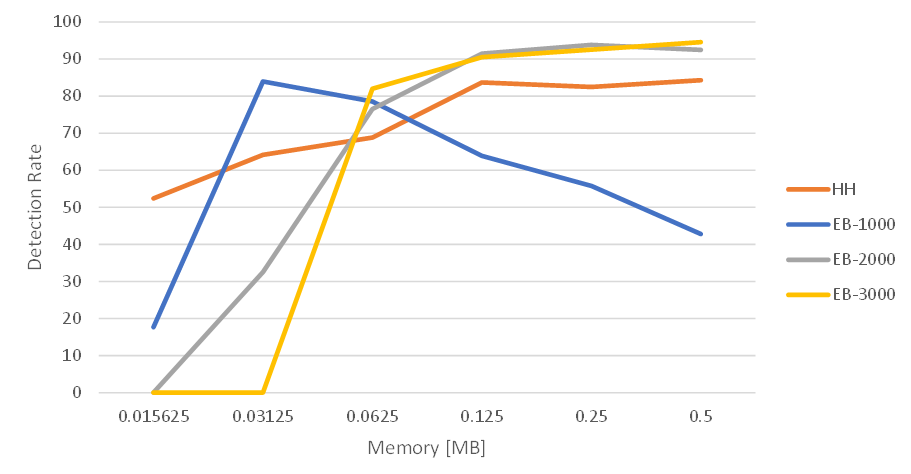
\includegraphics[width=\linewidth]{HH/figures/EB.png}
    \caption[Average Detection Rate of \cs\ and the \eb\ algorithms]{The Average Detection Rate as function of memory, comparing our the \cs\ algorithm and the \eb\ algorithm with different sizes of banks ($\phi=0.001,\delta=0.05m N=10^7, m_{CS}=0.5, m_{SEA}=0.01$)}
    \label{figure5}
\end{figure}

Figure~\ref{figure5} compares the DR of the \cs\ algorithm with the \eb\ algorithm with three sizes of banks 1000, 2000, and 3000. Since every 1000 entries in the \eb\ algorithm require around $16KB$, the algorithm suffers from poor DR in the smaller ranges of the memory. However, once the memory allows a decent size of the \sfa, the \eb\ algorithm starts to perform better since many more HH flows are propagating to the bank and have now an exact estimation up to the \pe\ introduced by the \sfa. One should note, that for \eb\ with size 1000 the DR becomes poor once again the larger the \sfa, that is since larger \sfa\ is propagating too many flows to the \eb\ and without an eviction. It is important to note, this higher DR comes with a cost of lower throughput and higher FPR since it performs a linear search in the size of the bank (which is constant) and it returns all flows in the \eb\ as potential HH.
\section{Conclusions}
\label{sec:conclusions}

In this chapter, we presented a new algorithm for  detecting Heavy Hitter flows.  Our algorithm   performs better than the state of art algorithm for practical sizes of available on device memory. The estimated frequency reported by the algorithm is in the range of $1\pm \delta$ from their actual frequency. Furthermore, we evaluated our algorithm on real internet traces and showed that it performs better, in terms of Detection Rate, False Positive Ratio and Throughput, than best existing  algorithms in various settings. More specifically, when processing $10^7$ packets our algorithm performs better for any amount of memory less than $1MB$. This also holds for $10^6, 10^5$ packets with memories of $0.5MB, 0.25MB$ respectively.

% \include{main/prelims}
% \include{main/mainchap1}
% \chapter{Conclusions and Future Directions}
\label{chap:conclusion}

In this dissertation, we presented our point of view of what should be considered a practical, efficient, and resource-constrained monitoring algorithm. We presented such algorithms for three famous problems in the domain of network monitoring, the top-$k$ problem, the Hierarchical Heavy Hitter Problem, and the Heavy Hitter problem. For each of these problems we surveyed the state of the art algorithms and identified their impracticality constraints. Afterward, we compared the performance of our algorithms against the state of the art algorithms on real internet traces and showed that they perform and at least as good as the state of the art algorithms, and for some settings even better, for the lower end of the range of available memory without suffering their impracticality constrains. 

In Chapter~\ref{cha:topk}, we introduced a family of practical, efficient memory-constrained algorithms for detecting the top-$k$ flows in terms of total traffic rate. These algorithms use built-in counters available in any switching node and are deployable “out of the box” on any OpenFlow enabled node. We evaluated the expected performance of these algorithms using real-life packet traces, and the evaluation shows that our new algorithms achieve high detection rates while maintaining full precision regardless of the packet rate. We also show that for the top-$k$ packet rate problem these algorithms perform as well as the best streaming algorithms that use complex data structures and much more elaborated computations. Moreover, for the more relevant weighted top-$k$ problem our algorithms outperform state-of-the-art streaming algorithms when evaluated over recent real traffic. 

In Chapter~\ref{cha:HHH}, we presented several practical memory-constrained algorithms for Hierarchical Heavy Hitters detection. These algorithms can be deployed on off-the-shelf network nodes (or software devices) and can operate in line speed due to their $O(1)$ per-packet operation. The current state of the art algorithms, either requires $O(H)$ per-packet operation that makes them unfeasible to be deployed in line rate or requires a convergence interval before reporting satisfactory results which makes them less relevant in many practical settings. On the contrary, our algorithms perform in line-speed with $O(1)$ update per-packet without requiring any convergence interval. Furthermore, no complex data structures are needed and our algorithms only require using built-in fast counters available in any network node.

We evaluated the algorithms on two recent real Internet packet traces and showed that they yield comparable results to the state of the art without their limitations. The evaluation showed that the best algorithm can detect up to 90\% of the HHH in a trace and report no more than 5\% non HHH flows.

These algorithms could be easily extended to the case of multi-dimensional HHH while keeping the depth of the hierarchy linear in the number of dimensions without modifying the $O(1)$ update time. Also, they allow practical detection of the weighted set of HHH flows with minimal modification of the update operations while keeping all of the algorithms promises.

In Chapter~\ref{cha:HH}, we introduced a new algorithm for detecting Heavy Hitter flows. Our algorithm performs better than the state of the art algorithms for practical sizes of memory available on devices. The estimated frequency reported by the algorithm is in the range of $1\pm \delta$ from their actual frequency. Furthermore, we evaluated our algorithm on real internet traces and showed that it performs better, in terms of Detection Rate, False Positive Ratio, and Throughput, than the best existing algorithms in various settings. More specifically, when processing $10^7$ packets our algorithm performs better for any amount of memory less than $1MB$. This also holds for $10^6, 10^5$ packets with memories of $0.5MB, 0.25MB$ respectively.

\section*{Future Directions}

One possible future direction of this work is to facilitate the presented algorithms as building-blocks for detecting network-wise top-$k$, Hierarchical Heavy Hitter, and Heavy Hitter flows. We believe that combining the local performance described in this document with a smart global policy about the number of counters or amount of memory to be used in each node, will lead to deployable memory-efficient network-wide monitoring systems. Furthermore, we believe that the study of the control mechanism in such a network-wide monitoring system will turn up to be of great importance to the system's efficiency and practicality.

%
% Add any appendices here; they must come _before_ the bibliography
%
\appendix
%\noappendicestocpagenum
%\addappheadtotoc
% \include{main/appendix1}

% Back Matter
% ------------

% The following command will typeset the bibliography,
% then typeset the Hebrew part of the thesis:
% - Cover page
% - Title page
% - Acknowledgements page
%  (NO table of contents or list of figures in Hebrew)
% - (Extended) abstract (1000-2000 words)
%
% based on information you've provided in the thesis-fields file
% (including the relative paths to your bib files). The Hebrew
% content will be typeset in _reverse_page_order_, i.e. first
% in the file will be the last page of the abstract, and the
% Hebrew cover page will be the last page of the file.
%
\makebackmatter

% The resulting PDF can be printed and taken straight to binding,
% i.e. you do not need to flip any pages anywhere. Of course,
% mind the LaTeX error and warning messages, overfull hboxes etc.

\end{document}

